% !TeX document-id = {852b5d47-4b9e-4872-84b9-4431b89a3313}
% !TeX program = xelatex
% !TeX TXS-program:compile = txs:///xelatex/[--shell-escape]
%%%%%%%%%%%%%%%%%%%%%%%%%%%%%%%%%%%%%%%%%%%%%%%%%%%%%%%%%%%%%%%%%%%%%%%%
% Plantilla TFG/TFM
% Escuela Politécnica Superior de la Universidad de Alicante
% Realizado por: Jose Manuel Requena Plens
% Contacto: info@jmrplens.com / Telegram:@jmrplens
%%%%%%%%%%%%%%%%%%%%%%%%%%%%%%%%%%%%%%%%%%%%%%%%%%%%%%%%%%%%%%%%%%%%%%%%

% Elige si deseas optimizar la ejecución del proyecto almacenando las figuras generadas con TikZ y PGF en una carpeta (archivos/figuras-procesadas).
% 1 - Si, 2 - No
\def\OptimizaTikZ{1}

% Archivo .TEX que incluye todas las configuraciones del documento y los paquetes. Añade todo aquello que necesites utilizar en el documento en este archivo.
% En él se encuentra la configuración de los márgenes, establecidos según las directrices de estilo de la EPS.
%%%%%%%%%%%%%%%%%%%%%%%%%%%%%%%%%%%%%%%%%%%%%%%%%%%%%%%%%%%%%%%%%%%%%%%%
% Plantilla TFG/TFM
% Escuela Politécnica Superior de la Universidad de Alicante
% Realizado por: Jose Manuel Requena Plens
% Contacto: info@jmrplens.com / Telegram:@jmrplens
%%%%%%%%%%%%%%%%%%%%%%%%%%%%%%%%%%%%%%%%%%%%%%%%%%%%%%%%%%%%%%%%%%%%%%%%

%%%%%%%%%%%%%%%%%%%%%%%%
% FORMATO DEL DOCUMENTO
%%%%%%%%%%%%%%%%%%%%%%%%
% scrbook es la clase de documento
% Si se desea que no haya página en blanco entre capítulos añadir "openany" en los parámetros de la clase. Sino siempre los capítulos empezarán en página impar.
\documentclass[a4paper,11pt,titlepage]{scrbook}
\KOMAoption{toc}{bib,chapterentryfill} % Opciones del índice
\usepackage{scrhack} % Previene algunos errores
% Paquete de formato para scrbook. Con marcas, linea-separador superior e inferior
\usepackage[automark,headsepline,footsepline]{scrlayer-scrpage}
\clearpairofpagestyles		% Borra los estilos por defecto
%%
% Formato y contenido de la información de cabecera y pie de página
%%
% Información de capítulo en cabecera e interno
\ihead{{\color{gray30}\scshape\small\headmark}}	
% Número de página en cabecera y externo
\ohead{\normalfont\pagemark} 
% Número de página en pie de página y externo. Sólo en páginas sin cabecera
\ofoot[\normalfont\pagemark]{}
%% 		
% Edición del contenido de las distintas partes de la cabecera
%%
\renewcommand{\chaptermark}[1]{\markboth{#1}{}} % Capítulo (Solo texto)
\renewcommand{\sectionmark}[1]{\markright{\thesection. #1}} % Sección (Número y texto)
\setkomafont{pagenumber}{} % Número de página (Sin nada añadido)

% Añade al índice y numera hasta la profundidad 4.
% 1:section,2:subsection,3:subsubsection,4:paragraph
\setcounter{tocdepth}{4}
\setcounter{secnumdepth}{4}
% Muestra una regla para comprobar el formato de las páginas
%\usepackage[type=upperleft,showframe,marklength=8mm]{fgruler}
% MÁRGENES DE LAS PÁGINAS
\usepackage[
  inner	=	3.0cm, % Margen interior
  outer	=	2.5cm, % Margen exterior
  top	=	2.5cm, % Margen superior
  bottom=	2.5cm, % Margen inferior
  includeheadfoot, % Incluye cabecera y pie de página en los márgenes
]{geometry}
% Valor de interlineado
\renewcommand{\baselinestretch}{1.0} % 1 línea de interlineado
% Para poder generar páginas horizontales
\usepackage{lscape}
% Ancho de la zona para comentarios en el margen. (modificado para todonotes)
\setlength{\marginparwidth}{1.9cm}

%%%%%%%%%%%%%%%%%%%%%%%%
% BIBLIOGRAFÍA
%%%%%%%%%%%%%%%%%%%%%%%%
\usepackage{apacite} % NORMA APA
\usepackage{natbib}
\usepackage{breakcites}

%%%%%%%%%%%%%%%%%%%%%%%%
% DOCUMENTO EN ESPAÑOL
%%%%%%%%%%%%%%%%%%%%%%%%
\usepackage[base]{babel}
\usepackage{polyglossia}
\setdefaultlanguage{spanish}

\addto\captionsspanish{%
	\renewcommand{\listtablename}{Índice de tablas} 
	\renewcommand{\tablename}{Tabla}
	\renewcommand{\lstlistingname}{Código}
	\renewcommand{\lstlistlistingname}{Índice de \lstlistingname s}
	\renewcommand{\glossaryname}{Glosario}
	\renewcommand{\acronymname}{Acrónimos}
	\renewcommand{\bibname}{Bibliografía}%
}

%%%%%%%%%%%%%%%%%%%%%%%% 
% COLORES
%%%%%%%%%%%%%%%%%%%%%%%% 
% Biblioteca de colores
\usepackage{color}
\usepackage[dvipsnames]{xcolor}
% Otros colores definidos por el usuario
\definecolor{gray97}{gray}{.97}
\definecolor{gray75}{gray}{.75}
\definecolor{gray45}{gray}{.45}
\definecolor{gray30}{gray}{.30}
\definecolor{negro}{RGB}{0,0,0}
\definecolor{blanco}{RGB}{255,255,255}
\definecolor{dkgreen}{rgb}{0,.6,0}
\definecolor{dkblue}{rgb}{0,0,.6}
\definecolor{dkyellow}{cmyk}{0,0,.8,.3}
\definecolor{gray}{rgb}{0.5,0.5,0.5}
\definecolor{mauve}{rgb}{0.58,0,0.82}
\definecolor{deepblue}{rgb}{0,0,0.5}
\definecolor{deepred}{rgb}{0.6,0,0}
\definecolor{deepgreen}{rgb}{0,0.5,0}
\definecolor{MyDarkGreen}{rgb}{0.0,0.4,0.0}
\definecolor{bluekeywords}{rgb}{0.13,0.13,1}
\definecolor{greencomments}{rgb}{0,0.5,0}
\definecolor{redstrings}{rgb}{0.9,0,0}

%%%%%%%%%%%%%%%%%%%%%%%%
% TABLAS
%%%%%%%%%%%%%%%%%%%%%%%%
% Paquetes para tablas
\usepackage{longtable,booktabs,array,multirow,multicol,tabularx,ragged2e,array}
% Nuevos tipos de columna para tabla, se pueden utilizar como por ejemplo C{3cm} en la definición de columnas de la función tabular
\newcolumntype{L}[1]{>{\raggedright\let\newline\\\arraybackslash\hspace{0pt}}m{#1}}
\newcolumntype{C}[1]{>{\centering\let\newline\\\arraybackslash\hspace{0pt}}m{#1}}
\newcolumntype{R}[1]{>{\raggedleft\let\newline\\\arraybackslash\hspace{0pt}}m{#1}}

%%%%%%%%%%%%%%%%%%%%%%%% 
% GRAFICAS y DIAGRAMAS 
%%%%%%%%%%%%%%%%%%%%%%%% 
% Paquete para todo tipo de gráficas, diagramas, modificación de imágenes, etc
\usepackage{tikz,tikzpagenodes}
\usetikzlibrary{tikzmark,calc,shapes.geometric,arrows,backgrounds,shadings,shapes.arrows,shapes.symbols,shadows,positioning,fit,automata,patterns,intersections}
\usepackage{pgfplots}
\pgfplotsset{colormap/jet}
\pgfplotsset{compat=newest} % Compatibilidad
\usepgfplotslibrary{patchplots,groupplots,fillbetween,polar}
\usepackage{pgfplotstable}
% Guardar las figuras realizadas con Tikz y Pgf en una carpeta externa
% para agilizar el procesado y tenerlas para utilizarlas en otros
% documentos
\if\OptimizaTikZ 1
\usepgfplotslibrary{external}
\tikzexternalize[prefix=archivos/figuras-procesadas/] % Ruta
\tikzset{%
    external/system call ={xelatex -enable-write18 -halt-on-error -interaction=batchmode -jobname "\image" "\texsource"},
}
\fi

% Estilos para elementos graficos
% Cajas y cajas de texto
\tikzstyle{Caja1} = [green,very thick,rounded corners,fill=white, fill opacity=0.5]
\tikzstyle{Texto1} = [fill=white,thick,shape=circle,draw=black,inner sep=2pt,font=\sffamily,text=black]
\tikzstyle{Texto2} = [fill=white,thick,shape=rectangle,draw=black,inner sep=2pt,font=\sffamily,text=black]
\tikzstyle{Texto3} = [fill=white,thick,shape=circle,draw=black,inner sep=2pt,font=\sffamily,text=black]
% Cuadros de diagrama
\tikzstyle{rectvioleta} = [rectangle, rounded corners, text centered, draw=black, fill=blue!10]
\tikzstyle{rectnaranja} = [rectangle, minimum width=2cm, minimum height=1cm, text centered, draw=black, fill=orange!10]
\tikzstyle{romborosa} = [diamond, aspect=3, minimum width=3cm, minimum height=1cm, text centered, draw=black, fill=red!10]
\tikzstyle{rectverde} = [rectangle, minimum width=2cm, minimum height=1cm, text centered, draw=black, fill=green!10]
\tikzstyle{rectamarillo} = [rectangle, rounded corners, minimum width=2cm, minimum height=1cm, text centered, draw=black, fill=yellow!10]
% Flechas
\tikzstyle{arrow} = [thick,->,>=stealth]

%%%%%%%%%%%%%%%%%%%%%%%% 
% FIGURAS, TABLAS, ETC 
%%%%%%%%%%%%%%%%%%%%%%%% 
\usepackage{subcaption} % Para poder realizar subfiguras
\usepackage{caption} % Para aumentar las opciones de diseño
% Nombres de figuras, tablas, etc, en negrita la numeración, todo con letra small
\captionsetup{labelfont={bf,small},textfont=small}
% Paquete para modificar los espacios arriba y abajo de una figura o tabla
\usepackage{setspace}
% Define el espacio tanto arriba como abajo de las figuras, tablas
\setlength{\intextsep}{5mm}
% Para ajustar tamaños de texto de toda una tabla o grafica
% Uso: {\scalefont{0.8} \begin{...} \end{...} }
\usepackage{scalefnt}
% Redefine las tablas y figuras para eliminar el '.' entre la numeración y el texto
\renewcommand*{\figureformat}{\figurename~\thefigure}
\renewcommand*{\tableformat}{\tablename~\thetable}

%%%%%%%%%%%%%%%%%%%%%%%% 
% TEXTO
%%%%%%%%%%%%%%%%%%%%%%%%
% Paquete para poder modificar las fuente de texto
\usepackage{xltxtra}
% Cualquier tamaño de texto. Uso: {\fontsize{100pt}{120pt}\selectfont tutexto}
\usepackage{anyfontsize}
% Para modificar parametros del texto.
\usepackage{setspace}
% Paquete para posicionar bloques de texto
\usepackage{textpos}
% Paquete para realizar cajas de texto. 
% Uso: \begin{mdframed}[linecolor=red!100!black] tutexto \end{mdframed}
\usepackage{framed,mdframed}
% Para subrayar. Uso: \hlc[tucolor]{tutexto}
\newcommand{\hlc}[2][yellow]{ {\sethlcolor{#1} \hl{#2}} }

%%%%%%%%%%%%%%%%%%%%%%%% 
% OTROS
%%%%%%%%%%%%%%%%%%%%%%%%
% Para hacer una pagina horizontal. Uso: \begin{landscape} xxxx \end{lanscape}
\usepackage{lscape} 
% Para incluir paginas PDF. Uso:
% \includepdf[pages={1}]{tuarchivo.pdf}
\usepackage{pdfpages}
% Para introducir url's con formato. Uso: \url{http://www.google.es}
\usepackage{url}
% Amplia muchas funciones graficas de latex
\usepackage{graphicx}
% Paquete que añade el hipervinculo en referencias dentro del documento, indice, etc
% Se define sin bordes alrededor. Uso: \ref{tulabel}
\usepackage[pdfborder={000}]{hyperref}
\usepackage{float}
\usepackage{placeins}
\usepackage{afterpage}
\usepackage{verbatim}
% Paquete para condicionales avanzados
\usepackage{xstring,xifthen}
% Paquete para realizar calculos en el código
\usepackage{calc}
% Para rotar tablas o figuras o su contenido
\usepackage{rotating} 
% Para incluir comentarios en el texto. El parámetro 'disable' oculta todas las notas.
% USO: \todo{tutexto}
\usepackage[textsize=tiny,spanish,shadow,textwidth=2cm]{todonotes}
%\reversemarginpar % Descomentar si se quiere todos los comentarios en el mismo lado
% Desactiva la exportación de los ToDo y Missingfigures como figuras
\if\OptimizaTikZ 1
\makeatletter
\renewcommand{\todo}[2][]{\tikzexternaldisable\@todo[#1]{#2}\tikzexternalenable}
\makeatother
\usepackage{letltxmacro}
\LetLtxMacro{\oldmissingfigure}{\missingfigure}
\makeatletter
\renewcommand{\missingfigure}[2][]{\tikzexternaldisable\oldmissingfigure[{#1}]{#2}\tikzexternalenable}
\makeatother
\fi

%%%%%%%%%%%%%%%%%%%%%%%% 
% GLOSARIOS
%%%%%%%%%%%%%%%%%%%%%%%%
\usepackage[acronym,nonumberlist,toc]{glossaries}
\usepackage{glossary-superragged}
\newglossarystyle{modsuper}{%
  \setglossarystyle{super}%
  \renewcommand{\glsgroupskip}{}
}
\renewcommand{\glsnamefont}[1]{\textbf{#1}}


%%%%%%%%%%%%%%%%%%%%%%%% 
% COMANDOS AÑADIDOS
%%%%%%%%%%%%%%%%%%%%%%%%
% Para mostrar la fecha actual (mes año) con \Hoy
\newcommand{\MES}{%
  \ifcase\month% 0
    \or Enero% 1
    \or Febrero% 2
    \or Marzo% 3
    \or Abril% 4
    \or Mayo% 5
    \or Junio% 6
    \or Julio% 7
    \or Agosto% 8
    \or Septiembre% 9
    \or Octubre% 10
    \or Noviembre% 11
    \or Diciembre% 12
  \fi}
\newcommand{\ANYO}{\number\year}
\newcommand{\Hoy}{\MES\ \ANYO}

%%%%%%%%%%%%%%%%%%%%%%%% 
% MATEMÁTICAS
%%%%%%%%%%%%%%%%%%%%%%%%
\usepackage{mathtools,amsthm,amsfonts,amssymb,bm,mathrsfs,nicefrac,upgreek,bigints} 
% Comando para añadir información de variables a las ecuaciones
% Uso: \begin{condiciones}[donde:] ....... \end{condiciones}
\newenvironment{condiciones}[1][2]
  {%
   #1\tabularx{\textwidth-\widthof{#1}}[t]{
     >{$}l<{$} @{}>{${}}c<{{}$}@{} >{\raggedright\arraybackslash}X
   }%
  }
  {\endtabularx\\[\belowdisplayskip]}

%%%%%
% PARÁMETROS DE FORMATO DE CODIGOS
%%%%%
% Puedes editar los formatos para ajustarlos a tu gusto
%%%%%%%%%%%%%%%%%%%%%%%%%%%%%%%%%%%%%%%%%%%%%%%%%%%%%%%%%%%%%%%%%%%%%%%%
% Plantilla TFG/TFM
% Escuela Politécnica Superior de la Universidad de Alicante
% Realizado por: Jose Manuel Requena Plens
% Contacto: info@jmrplens.com / Telegram:@jmrplens
%%%%%%%%%%%%%%%%%%%%%%%%%%%%%%%%%%%%%%%%%%%%%%%%%%%%%%%%%%%%%%%%%%%%%%%%


%%%%%%%%%%%%%%%%%%%%%%%% 
% CÓDIGO. CONFIGURACIÓN. En el siguiente bloque están los estilos.
%%%%%%%%%%%%%%%%%%%%%%%%
% Paquete para mostrar código de matlab. En caja y lineas numeradas
\usepackage[framed,numbered]{matlab-prettifier}
% Paquete mostrar código de programación de distintos lenguajes
\usepackage{listings}
\lstset{ inputencoding=utf8,
extendedchars=true,
frame=single, % Caja donde se ubica el código
backgroundcolor=\color{gray97}, % Color del fondo de la caja
rulesepcolor=\color{black},
boxpos=c,
abovecaptionskip=-4pt,
aboveskip=12pt,
belowskip=0pt,
lineskip=0pt,
framerule=0pt,
framextopmargin=4pt,
framexbottommargin=4pt,
framexleftmargin=11pt,
framexrightmargin=0pt,
linewidth=\linewidth,
xleftmargin=\parindent,
framesep=0pt,
rulesep=.4pt,
stringstyle=\ttfamily,
showstringspaces = false,
showspaces = false,
showtabs = false,
columns=fullflexible,
basicstyle=\small\ttfamily,
commentstyle=\color{gray45},
keywordstyle=\bfseries,
tabsize=4,
numbers=left,
numbersep=1pt,
numberstyle=\tiny\ttfamily\color{gray75},
numberfirstline = false,
breaklines=true,
postbreak=\mbox{\textcolor{red}{$\hookrightarrow$}\space}, % Flecha al saltar de linea
prebreak=\mbox{\textcolor{red}{$\hookleftarrow$}\space}, % Flecha al saltar de linea
literate=
  {á}{{\'a}}1 {é}{{\'e}}1 {í}{{\'i}}1 {ó}{{\'o}}1 {ú}{{\'u}}1
  {Á}{{\'A}}1 {É}{{\'E}}1 {Í}{{\'I}}1 {Ó}{{\'O}}1 {Ú}{{\'U}}1
  {à}{{\`a}}1 {è}{{\`e}}1 {ì}{{\`i}}1 {ò}{{\`o}}1 {ù}{{\`u}}1
  {À}{{\`A}}1 {È}{{\'E}}1 {Ì}{{\`I}}1 {Ò}{{\`O}}1 {Ù}{{\`U}}1
  {ä}{{\"a}}1 {ë}{{\"e}}1 {ï}{{\"i}}1 {ö}{{\"o}}1 {ü}{{\"u}}1
  {Ä}{{\"A}}1 {Ë}{{\"E}}1 {Ï}{{\"I}}1 {Ö}{{\"O}}1 {Ü}{{\"U}}1
  {â}{{\^a}}1 {ê}{{\^e}}1 {î}{{\^i}}1 {ô}{{\^o}}1 {û}{{\^u}}1
  {Â}{{\^A}}1 {Ê}{{\^E}}1 {Î}{{\^I}}1 {Ô}{{\^O}}1 {Û}{{\^U}}1
  {œ}{{\oe}}1 {Œ}{{\OE}}1 {æ}{{\ae}}1 {Æ}{{\AE}}1 {ß}{{\ss}}1
  {ű}{{\H{u}}}1 {Ű}{{\H{U}}}1 {ő}{{\H{o}}}1 {Ő}{{\H{O}}}1
  {ç}{{\c c}}1 {Ç}{{\c C}}1 {ø}{{\o}}1 {å}{{\r a}}1 {Å}{{\r A}}1
  {€}{{\euro}}1 {£}{{\pounds}}1 {«}{{\guillemotleft}}1
  {»}{{\guillemotright}}1 {ñ}{{\~n}}1 {Ñ}{{\~N}}1 {¿}{{?`}}1,
  }

% Intenta no dividir los códigos en diferentes paginas si es posible
\lstnewenvironment{listing}[1][]
   {\lstset{#1}\pagebreak[0]}{\pagebreak[0]}

% Formato de títulos de los códigos
\DeclareCaptionFont{white}{\color{white}}
\DeclareCaptionFormat{listing}{\colorbox{gray}{\parbox{\textwidth - 2\fboxsep}{#1#2#3}}}
\captionsetup[lstlisting]{format=listing,labelfont=white,textfont=white,font= scriptsize}


%%%%%%%%%%%%%%%%%%%%%%%% 
% CÓDIGO. ESTILOS. Ajústalos a tu gusto
%%%%%%%%%%%%%%%%%%%%%%%%
\lstdefinestyle{Consola}
	{
	basicstyle=\scriptsize\bfseries\ttfamily,
	}
   
\lstdefinestyle{C}
	{
	basicstyle=\scriptsize,
	language=C,
	}
\lstdefinestyle{C-color}
	{
  	breaklines=true,
  	language=C,
  	basicstyle=\scriptsize,
  	keywordstyle=\bfseries\color{green!40!black},
  	commentstyle=\itshape\color{purple!40!black},
  	identifierstyle=\color{blue},
  	stringstyle=\color{orange},
    }
\lstdefinestyle{CSharp}
	{
	basicstyle=\scriptsize,
	language=[Sharp]C,
	escapeinside={(*@}{@*)},
	keywordstyle=\bfseries,
	}
\lstdefinestyle{CSharp-color}
	{
	basicstyle=\scriptsize,
	language=[Sharp]C,
	escapeinside={(*@}{@*)},
	commentstyle=\color{greencomments},
	keywordstyle=\color{bluekeywords}\bfseries,
	stringstyle=\color{redstrings},
	}
\lstdefinestyle{C++}
	{
	basicstyle=\scriptsize,
	language=C++,
 	}
 	
\lstdefinestyle{C++-color}
	{
  	breaklines=true,
  	language=C++,
  	basicstyle=\scriptsize,
  	keywordstyle=\bfseries\color{green!40!black},
  	commentstyle=\itshape\color{purple!40!black},
  	identifierstyle=\color{blue},
  	stringstyle=\color{orange},
    }
    
\lstdefinestyle{PHP}
	{
	basicstyle=\scriptsize,
	language=PHP,
	}
	
\lstdefinestyle{PHP-color}
	{
	basicstyle=\scriptsize,
	language=PHP,
	keywordstyle    = \color{dkblue},
  	stringstyle     = \color{red},
  	identifierstyle = \color{dkgreen},
  	commentstyle    = \color{gray},
  	emph            =[1]{php},
  	emphstyle       =[1]\color{black},
  	emph            =[2]{if,and,or,else},
  	emphstyle       =[2]\color{dkyellow}
  }
  
\lstdefinestyle{Matlab}
	{
	basicstyle=\scriptsize,
	language=Matlab,
	numberstyle=\tiny\ttfamily\color{gray75},
	}
	
\lstdefinestyle{Matlab-color}
	{
	style = Matlab-editor,
	basicstyle=\scriptsize,
	numberstyle=\tiny\ttfamily\color{gray75},
	}
	
\lstdefinestyle{Latex}
	{
	language=[LaTeX]{Tex},
    basicstyle=\scriptsize,
    literate={\$}{{{\bfseries\$}}}1,
    alsoletter={\\,*,\&},
    emph =[1]{\\begin,\\end,\\caption,\\label,\\centering,\\FloatBarrier,
              \\lstinputlisting,\\scalefont,\\addplot,\\input,
              \\legend,\\item,\\subitem,\\includegraphics,\\textwidth,
              \\section,\\subsection,\\subsubsection,\\paragraph,
              \\cite,\\citet,\\citep,\\gls,\\bibliographystyle,\\url,
              \\citet*,\\citep*,\\todo,\\missingfigure,\\footnote},
  	emphstyle =[1]\bfseries,
  	emph = [2]{equation,subequations,eqnarray,figure,subfigure,
  			   condiciones,flalign,tikzpicture,axis,lstlisting,
  			   itemize,description
  			   },
  	emphstyle =[2]\bfseries,
    numbers=none,
	}
	
\lstdefinestyle{Latex-color}
	{
	language=[LaTeX]{Tex},
    basicstyle=\scriptsize,
    commentstyle=\color{dkgreen},
    identifierstyle=\color{black},
    literate={\$}{{{\bfseries\color{Dandelion}\$}}}1, % Colorea el simbolo dollar
    alsoletter={\\,*,\&},
    emph =[1]{\\begin,\\end,\\caption,\\label,\\centering,\\FloatBarrier,
              \\lstinputlisting,\\scalefont,\\addplot,\\input,
              \\legend,\\item,\\subitem,\\includegraphics,\\textwidth,
              \\section,\\subsection,\\subsubsection,\\paragraph,
              \\cite,\\citet,\\citep,\\gls,\\bibliographystyle,\\url,
              \\citet*,\\citep*,\\todo,\\missingfigure,\\footnote},
  	emphstyle =[1]\bfseries\color{RoyalBlue},
  	emph = [2]{equation,subequations,eqnarray,figure,subfigure,
  			   condiciones,flalign,tikzpicture,axis,lstlisting,
  			   itemize,description
  			   },
  	emphstyle =[2]\bfseries,
    numbers=none,
	}
\lstdefinestyle{Java}
{
	basicstyle=\scriptsize,
	language=Java,
}

\lstdefinestyle{Java-color}
{
	basicstyle=\scriptsize,
	language=Java,
  	keywordstyle=\color{blue},
  	commentstyle=\color{dkgreen},
  	stringstyle=\color{mauve},
}
\lstdefinestyle{Python}
{
	language=Python,
	basicstyle=\scriptsize,
	otherkeywords={self},  
	keywordstyle=\bfseries,     
	emphstyle=\bfseries,    
	emph={MyClass,__init__},         
}

\lstdefinestyle{Python-color}
{
	language=Python,
	basicstyle=\scriptsize,
	otherkeywords={self},          
	keywordstyle=\bfseries\color{deepblue},
	emph={MyClass,__init__},         
	emphstyle=\bfseries\color{deepred},    
	stringstyle=\color{deepgreen},
}
\lstdefinestyle{R}
{
	language=R,                     
  	basicstyle=\scriptsize,
  	keywordstyle=\bfseries, 
}
\lstdefinestyle{R-color}
{
	language=R,                     
  	basicstyle=\scriptsize,
  	keywordstyle=\bfseries\color{RoyalBlue}, 
  	commentstyle=\color{YellowGreen},
  	stringstyle=\color{ForestGreen}  
}


%%%%%
% DEFINICION DE CONCEPTOS
%%%%
% Uso ejemplo: \begin{ejemplo} tucontenido \end{ejemplo} 
\newtheorem{teorema}{Teorema}[chapter]
\newtheorem{ejemplo}{Ejemplo}[chapter]
\newtheorem{definicion}{Definición}[chapter]



%%%%%%%%%%%%%%%%%%%%%%%%%%%%%%%%%%%%%%%%%%%%%%%%%%%%%%%%%%%%%%%%%%%%%%
% INFORMACIÓN DEL TFG
% Comentar lo que NO se desee añadir y sustituir con la información correcta.
%%%%%%%%%%%%%%%%%%%%%%%%%%%%%%%%%%%%%%%%%%%%%%%%%%%%%%%%%%%%%%%%%%%%%%
% Título y subtítulo
\newcommand{\titulo}{Tecnología de Videojuegos y Machine Learning desde cero}
\newcommand{\subtitulo}{}
% Datos del autor
\newcommand{\miNombre}{Arturo Juan Martínez Sánchez}
% Determinar género para etiquetas Autore/Autora/Autor (nb o en blanco,f,m)
\newcommand{\miGenero}{m}
\newcommand{\miEmail}{ajms3@alu.ua.es}
% Datos del tutor/es
% Si no hay tutorB, comentar tutorB y dptoB para que la etiqueta sea Tutor:
\newcommand{\miTutor}{Francisco Jose Gallego Duran}
% \newcommand{\miTutorB}{Nombre Apellido1 Apellido2 (tutor2)}
\newcommand{\departamentoTutor}{B161 CIENCIA DE LA COMPUTACION E INTELIGENCIA ARTIFICIAL}
% \newcommand{\departamentoTutorB}{Departamento del cotutor}
% Datos de la facultad y universidad
\newcommand{\miFacultad}{Escuela Politécnica Superior}
\newcommand{\miFacultadCorto}{EPS UA}
\newcommand{\miUniversidad}{\protect{Universidad de Alicante}}
\newcommand{\miUbicacion}{Alicante}

%%%%%%%%%%%%%%%%%%%%%%%%%%%%%%%%%%%%%%%%%%%%%%%%%%%%%%%%%%%%%%%%%%%%%%
% INDICA TU TITULACIÓN
% ID	GRADO -------------------------------------------------
% 1		Ingeniería en Imagen y Sonido en Telecomunicación
% 2		Ingeniería Civil
% 3		Ingeniería Química
% 4		Ingeniería Informática
% 5		Ingeniería Multimedia
% 6		Arquitectura Técnica
% 7		Arquitectura
% 8		Robótica
% %		%%%%%%%%%%%%
% ID	MÁSTER ------------------------------------------------
% A		Telecomunicación
% B		Caminos, Canales y Puertos
% C		Gestión en la Edificación
% D		Desarrollo Web
% E		Materiales, Agua, Terreno
% F		Informática
% G 	Automática y Robótica
% H		Prevención de riesgos laborales
% I		Gestión Sostenible Agua
% J		Desarrollo Aplicaciones Móviles
% K		Ingeniería Química
% L		Ciberseguridad
%%%%%%%%%%%%%%%%%%%%%%%%%%%%%%%%%%%%%%%%%%%%%%%%%%%%%%%%%%%%%%%%%%%%%%%%%
%!!!!!!!!!!!!!!!!!!!!!!!!!!!!!!!!!!!!!!!!!!!!!!!!!!!!!!!!!!!!!!!!!!!!!%%%
																		%
\def\IDtitulo{4} % INTRODUCE LA ID DE TU TITULACIÓN						%
																		%
%!!!!!!!!!!!!!!!!!!!!!!!!!!!!!!!!!!!!!!!!!!!!!!!!!!!!!!!!!!!!!!!!!!!!!%%%
%%%%%%%%%%%%%%%%%%%%%%%%%%%%%%%%%%%%%%%%%%%%%%%%%%%%%%%%%%%%%%%%%%%%%%%%%

% Configuración automática según el identificador elegido
%%%%%%%%%%%%%%%%%%%%%%%%%%%%%%%%%%%%%%%%%%%%%%%%%%%%%%%%%%%%%%%%%%%%%%%%
% Plantilla TFG/TFM
% Escuela Politécnica Superior de la Universidad de Alicante
% Realizado por: Jose Manuel Requena Plens
% Contacto: info@jmrplens.com / Telegram:@jmrplens
%%%%%%%%%%%%%%%%%%%%%%%%%%%%%%%%%%%%%%%%%%%%%%%%%%%%%%%%%%%%%%%%%%%%%%%%

%%%%%%%%%%%%%%%%%%%%%%%% 
% COLORES DE GRADOS.
% Si el color de la titulación ha cambiado, modifícalo en las lineas siguientes.
%%%%%%%%%%%%%%%%%%%%%%%%
% Grados
\definecolor{teleco}{RGB}{32,2,116}			% Teleco
\definecolor{civil}{RGB}{201,56,140}			% Civil
\definecolor{quimica}{RGB}{41,199,255}		% Química
\definecolor{informatica}{RGB}{0,128,255}	% Informatica
\definecolor{multimedia}{RGB}{239,206,53}	% Multimedia
\definecolor{arquitecnica}{RGB}{0,179,148}	% Arquitectura técnica
\definecolor{arquitectura}{RGB}{181,0,0}		% Arquitectura
\definecolor{robotica}{RGB}{255,255,128}		% Robótica
% Másteres
\definecolor{masterteleco}{RGB}{32,2,116}	% Teleco
\definecolor{caminos}{RGB}{201,56,140}		% Caminos, Canales y Puertos
\definecolor{gestedif}{RGB}{50,120,50}		% Gestión Edificación
\definecolor{desweb}{RGB}{250,43,22}			% Desarrollo Web
\definecolor{mataguaterre}{RGB}{210,250,50}	% Materiales, Agua, Terreno
\definecolor{masterinfor}{RGB}{0,128,255}	% Informática
\definecolor{autorobo}{RGB}{83,145,201}		% Automática y Robótica
\definecolor{prevencion}{RGB}{0,100,0}		% Prevención Riesgos
\definecolor{gestionagua}{RGB}{7,138,197}	% Gestión Agua
\definecolor{moviles}{RGB}{121,11,21}		% Aplicaciones Móviles
\definecolor{masterquimica}{RGB}{41,199,255}	% Quimica
\definecolor{ciberseguridad}{RGB}{9,111,192}	% Ciberseguridad

% Logotipos comunes de todas las titulaciones
\newcommand{\logoFacultad}{include/logos-universidad/LogoEPSNegro}
\newcommand{\logoUniversidad}{include/logos-universidad/LogoUANegro}
\newcommand{\logoUniversidadPortada}{include/logos-universidad/LogoUABlanco}

% Colores generales
\definecolor{negro}{RGB}{0,0,0}
\definecolor{blanco}{RGB}{255,255,255}
%%%%%%%%%%%%%%%%%%%%%%%% 
% CONDICIONALES. SEGUN LA ID ELEGIDA EN EL .TEX PRINCIPAL
% Según el ID seleccionado en TFG_EPS_UA.tex se configurará el nombre de la titulación, logotipos y color.
% Si tu titulación no esta correctamente definida cambia las imágenes que se definen para tu titulación en las lineas de abajo
% Si deseas añadir mas titulaciones ve al final de este archivo
%%%%%%%%%%%%%%%%%%%%%%%%
% Grados
	\if\IDtitulo 1 % Teleco
		% Logos
		\newcommand{\logoFacultadPortada}{include/logos-universidad/LogoEPSBlanco}
		\newcommand{\logoGradoPortada}{include/logos-titulaciones/LogoTelecoBlanco}
		\newcommand{\logoGrado}{include/logos-titulaciones/LogoTelecoNegro}
		% Texto
		\newcommand{\miGrado}{Grado en Ingeniería en Sonido e Imagen en Telecomunicación}
		\newcommand{\tipotrabajo}{Trabajo Fin de Grado}
		% Color
		\newcommand{\colorgrado}{teleco}
		\newcommand{\colortexto}{blanco}
	\else \if\IDtitulo 2 % Civil
		\newcommand{\logoFacultadPortada}{include/logos-universidad/LogoEPSBlanco}
		\newcommand{\logoGradoPortada}{include/logos-titulaciones/LogoCivilBlanco}
		\newcommand{\logoGrado}{include/logos-titulaciones/LogoCivilNegro}
		% Texto
		\newcommand{\miGrado}{Grado en Ingeniería Civil}
		\newcommand{\tipotrabajo}{Trabajo Fin de Grado}
		% Color
		\newcommand{\colorgrado}{civil}
		\newcommand{\colortexto}{blanco}
	\else \if\IDtitulo 3 % Quimica
		% Logos
		\newcommand{\logoFacultadPortada}{include/logos-universidad/LogoEPSNegro}
		\newcommand{\logoGradoPortada}{include/logos-titulaciones/LogoQuimicaNegro}
		\newcommand{\logoGrado}{include/logos-titulaciones/LogoQuimicaNegro}
		% Texto
		\newcommand{\miGrado}{Grado en Ingeniería Química}
		\newcommand{\tipotrabajo}{Trabajo Fin de Grado}
		% Color
		\newcommand{\colorgrado}{quimica}
		\newcommand{\colortexto}{negro}
	\else \if\IDtitulo 4 % Informatica
		% Logos
		\newcommand{\logoFacultadPortada}{include/logos-universidad/LogoEPSBlanco}
		\newcommand{\logoGradoPortada}{include/logos-titulaciones/LogoInformaticaBlanco}
		\newcommand{\logoGrado}{include/logos-titulaciones/LogoInformaticaNegro}
		% Texto
		\newcommand{\miGrado}{Grado en Ingeniería Informática}
		\newcommand{\tipotrabajo}{Trabajo Fin de Grado}
		% Color
		\newcommand{\colorgrado}{informatica}
		\newcommand{\colortexto}{blanco}
	\else \if\IDtitulo 5 % Multimedia
		% Logos
		\newcommand{\logoFacultadPortada}{include/logos-universidad/LogoEPSNegro}
		\newcommand{\logoGradoPortada}{include/logos-titulaciones/LogoMultimediaNegro}
		\newcommand{\logoGrado}{include/logos-titulaciones/LogoMultimediaNegro}
		% Texto
		\newcommand{\miGrado}{Grado en Ingeniería Multimedia}
		\newcommand{\tipotrabajo}{Trabajo Fin de Grado}
		% Color
		\newcommand{\colorgrado}{multimedia}
		\newcommand{\colortexto}{negro}
	\else \if\IDtitulo 6 % Arquitectura Tecnica
		% Logos
		\newcommand{\logoFacultadPortada}{include/logos-universidad/LogoEPSBlanco}
		\newcommand{\logoGradoPortada}{include/logos-titulaciones/LogoArqTecnicaBlanco}
		\newcommand{\logoGrado}{include/logos-titulaciones/LogoArqTecnicaNegro}
		% Texto
		\newcommand{\miGrado}{Grado en Arquitectura Técnica}
		\newcommand{\tipotrabajo}{Trabajo Fin de Grado}
		% Color
		\newcommand{\colorgrado}{arquitecnica}
		\newcommand{\colortexto}{blanco}
	\else \if\IDtitulo 7 % Arquitectura
		% Logos
		\newcommand{\logoFacultadPortada}{include/logos-universidad/LogoEPSBlanco}
		\newcommand{\logoGradoPortada}{include/logos-titulaciones/LogoArquitecturaBlanco}
		\newcommand{\logoGrado}{include/logos-titulaciones/LogoArquitecturaNegro}
		% Texto
		\newcommand{\miGrado}{Grado en Arquitectura}
		\newcommand{\tipotrabajo}{Trabajo Fin de Grado}
		% Color
		\newcommand{\colorgrado}{arquitectura}
		\newcommand{\colortexto}{blanco}
	\else \if\IDtitulo 8 % Robotica
		% Logos
		\newcommand{\logoFacultadPortada}{include/logos-universidad/LogoEPSNegro}
		\newcommand{\logoGradoPortada}{include/logos-titulaciones/LogoRoboticaColor}
		\newcommand{\logoGrado}{include/logos-titulaciones/LogoRoboticaNegro}
		% Texto
		\newcommand{\miGrado}{Grado en Ingeniería Robótica}
		\newcommand{\tipotrabajo}{Trabajo Fin de Grado}
		% Color
		\newcommand{\colorgrado}{robotica}
		\newcommand{\colortexto}{negro}
% Másteres
	\else \if\IDtitulo A % Teleco
		% Logos
		\newcommand{\logoFacultadPortada}{include/logos-universidad/LogoEPSBlanco}
		\newcommand{\logoGradoPortada}{include/logos-titulaciones/LogoTelecoBlanco}
		\newcommand{\logoGrado}{include/logos-titulaciones/LogoTelecoNegro}
		% Texto
		\newcommand{\miGrado}{Máster Universitario en Ingeniería en Telecomunicación}
		\newcommand{\tipotrabajo}{Trabajo Fin de Máster}
		% Color
		\newcommand{\colorgrado}{masterteleco}
		\newcommand{\colortexto}{blanco}
	\else \if\IDtitulo B % Caminos, Canales y puertos
		% Logos
		\newcommand{\logoFacultadPortada}{include/logos-universidad/LogoEPSBlanco}
		\newcommand{\logoGradoPortada}{include/logos-titulaciones/LogoCivilBlanco}
		\newcommand{\logoGrado}{include/logos-titulaciones/LogoCivilNegro}
		% Texto
		\newcommand{\miGrado}{Máster Universitario en Ingeniería de Caminos, Canales y Puertos}
		\newcommand{\tipotrabajo}{Trabajo Fin de Máster}
		% Color
		\newcommand{\colorgrado}{caminos}
		\newcommand{\colortexto}{blanco}
	\else \if\IDtitulo C % Gestión Edificación
		% Logos
		\newcommand{\logoFacultadPortada}{include/logos-universidad/LogoEPSBlanco}
		\newcommand{\logoGradoPortada}{include/logos-titulaciones/LogoMasterEdificacionBlanco}
		\newcommand{\logoGrado}{include/logos-titulaciones/LogoMasterEdificacionNegro}
		\newcommand{\tipotrabajo}{Trabajo Fin de Máster}
		% Texto
		\newcommand{\miGrado}{Máster Universitario en Gestión de la Edificación}
		% Color
		\newcommand{\colorgrado}{gestedif}
		\newcommand{\colortexto}{blanco}
	\else \if\IDtitulo D % Desarrollo web
		% Logos
		\newcommand{\logoFacultadPortada}{include/logos-universidad/LogoEPSBlanco}
		\newcommand{\logoGradoPortada}{include/logos-titulaciones/LogoMasterDesarrolloBlanco}
		\newcommand{\logoGrado}{include/logos-titulaciones/LogoMasterDesarrolloNegro}
		% Texto
		\newcommand{\miGrado}{Máster Universitario en Desarrollo de Aplicaciones y Servicios Web}
		\newcommand{\tipotrabajo}{Trabajo Fin de Máster}
		% Color
		\newcommand{\colorgrado}{desweb}
		\newcommand{\colortexto}{blanco}
	\else \if\IDtitulo E % Materiales, Agua, Terreno
		% Logos
		\newcommand{\logoFacultadPortada}{include/logos-universidad/LogoEPSNegro}
		\newcommand{\logoGradoPortada}{include/logos-titulaciones/LogoMasterMaterialesNegro}
		\newcommand{\logoGrado}{include/logos-titulaciones/LogoMasterMaterialesNegro}
		% Texto
		\newcommand{\miGrado}{Máster Universitario en Ingeniería de los Materiales, del Agua y del Terreno}
		\newcommand{\tipotrabajo}{Trabajo Fin de Máster}
		% Color
		\newcommand{\colorgrado}{mataguaterre}
		\newcommand{\colortexto}{negro}
	\else \if\IDtitulo F % Informatica
		% Logos
		\newcommand{\logoFacultadPortada}{include/logos-universidad/LogoEPSBlanco}
		\newcommand{\logoGradoPortada}{include/logos-titulaciones/LogoInformaticaBlanco}
		\newcommand{\logoGrado}{include/logos-titulaciones/LogoInformaticaNegro}
		% Texto
		\newcommand{\miGrado}{Máster Universitario en Ingeniería Informática}
		\newcommand{\tipotrabajo}{Trabajo Fin de Máster}
		% Color
		\newcommand{\colorgrado}{masterinfor}
		\newcommand{\colortexto}{blanco}
	\else \if\IDtitulo G % Automática y Robótica
		% Logos
		\newcommand{\logoFacultadPortada}{include/logos-universidad/LogoEPSBlanco}
		\newcommand{\logoGradoPortada}{include/logos-titulaciones/LogoMasterRoboticaBlanco}
		\newcommand{\logoGrado}{include/logos-titulaciones/LogoMasterRoboticaNegro}
		% Texto
		\newcommand{\miGrado}{Máster Universitario en Automática y Robótica}
		\newcommand{\tipotrabajo}{Trabajo Fin de Máster}
		% Color
		\newcommand{\colorgrado}{autorobo}
		\newcommand{\colortexto}{blanco}
	\else \if\IDtitulo H % Prevención de riesgos laborales
		% Logos
		\newcommand{\logoFacultadPortada}{include/logos-universidad/LogoEPSBlanco}
		\newcommand{\logoGradoPortada}{include/logos-titulaciones/LogoMasterPrevencionBlanco}
		\newcommand{\logoGrado}{include/logos-titulaciones/LogoMasterPrevencionNegro}
		% Texto
		\newcommand{\miGrado}{Máster Universitario en Prevención de Riesgos Laborales}
		\newcommand{\tipotrabajo}{Trabajo Fin de Máster}
		% Color
		\newcommand{\colorgrado}{prevencion}
		\newcommand{\colortexto}{blanco}
	\else \if\IDtitulo I % Gestion Agua
		% Logos
		\newcommand{\logoFacultadPortada}{include/logos-universidad/LogoEPSNegro}
		\newcommand{\logoGradoPortada}{include/logos-titulaciones/LogoMasterAguaNegro}
		\newcommand{\logoGrado}{include/logos-titulaciones/LogoMasterAguaNegro}
		% Texto
		\newcommand{\miGrado}{Máster Universitario en Gestión Sostenible y Tecnologías del Agua}
		\newcommand{\tipotrabajo}{Trabajo Fin de Máster}
		% Color
		\newcommand{\colorgrado}{gestionagua}
		\newcommand{\colortexto}{negro}
	\else \if\IDtitulo J % Aplicaciones Móviles
		% Logos
		\newcommand{\logoFacultadPortada}{include/logos-universidad/LogoEPSBlanco}
		\newcommand{\logoGradoPortada}{include/logos-titulaciones/LogoMasterMovilesBlanco}
		\newcommand{\logoGrado}{include/logos-titulaciones/LogoMasterMovilesNegro}
		% Texto
		\newcommand{\miGrado}{Máster Universitario en Desarrollo de Software para Dispositivos Móviles}
		\newcommand{\tipotrabajo}{Trabajo Fin de Máster}
		% Color
		\newcommand{\colorgrado}{moviles}
		\newcommand{\colortexto}{blanco}
	\else \if\IDtitulo K % Quimica
		% Logos
		\newcommand{\logoFacultadPortada}{include/logos-universidad/LogoEPSNegro}
		\newcommand{\logoGradoPortada}{include/logos-titulaciones/LogoQuimicaNegro}
		\newcommand{\logoGrado}{include/logos-titulaciones/LogoQuimicaNegro}
		% Texto
		\newcommand{\miGrado}{Máster Universitario en Ingeniería Química}
		\newcommand{\tipotrabajo}{Trabajo Fin de Máster}
		% Color
		\newcommand{\colorgrado}{masterquimica}
		\newcommand{\colortexto}{negro}
	\else \if\IDtitulo L % Ciberseguridad
		% Logos
		\newcommand{\logoFacultadPortada}{include/logos-universidad/LogoEPSBlanco}
		\newcommand{\logoGradoPortada}{include/logos-titulaciones/LogoMasterCiberseguridadColor}
		\newcommand{\logoGrado}{include/logos-titulaciones/LogoMasterCiberseguridadNegro}
		% Texto
		\newcommand{\miGrado}{Máster Universitario en Ciberseguridad}
		\newcommand{\tipotrabajo}{Trabajo Fin de Máster}
		% Color
		\newcommand{\colorgrado}{ciberseguridad}
		\newcommand{\colortexto}{blanco}


	\fi \fi \fi \fi \fi \fi \fi \fi \fi \fi \fi \fi \fi \fi \fi \fi \fi \fi \fi \fi
	
%%%%%%%%%%%%%%%%%%%%%%%%%%%%%%%%%%%%%%%%%%%%%%%%%%%%%%%%%%%%%%%%%%%%%%%%	
% ¿COMO AÑADIR MÁS TITULACIONES?
% Para añadir más titulaciones, se debe continuar el el formato de ID -> Titulacion.
% Justo encima de la linea donde hay muchos '\fi' se debe escribir el condicional y el contenido de este tal que:
%
%	\else \if\IDtitulo X % Titulacion con ID=X		
% 		% Logos
%		\newcommand{\logoFacultadPortada}{include/logos-universidad/LogoEPSBlanco}
%		\newcommand{\logoGradoPortada}{include/logos-titulaciones/logotitulacion}
%		\newcommand{\logoGrado}{include/logos-titulaciones/logotitulacion}
%		% Texto
%		\newcommand{\miGrado}{Grado en XXXXXXXX}
%		\newcommand{\tipotrabajo}{Trabajo Fin de XXXX}
%		% Color
%		\newcommand{\colorgrado}{XXXX}
%		\newcommand{\colortexto}{XXX}
%	
% Por último añadir a la linea que tiene muchos '\fi', otro '\fi'. Listo, ya podrás usar la nueva ID con la configuración añadida.
%%%%%%%%%%%%%%%%%%%%%%%%%%%%%%%%%%%%%%%%%%%%%%%%%%%%%%%%%%%%%%%%%%%%%%%%	




 

% Información añadida a las propiedades del archivo PDF.
\hypersetup{
pdfauthor = {\miNombre~(\miEmail)},
pdftitle = {\titulo},
}

%%
% Archivo de acrónimos
%%
\makeglossaries % Genera la base de datos de acrónimos
%%%%%%%%%%%%%%%%%%%%%%%%%%%%%%%%%%%%%%%%%%%%%%%%%%%%%%%%%%%%%%%%%%%%%%%%
% Plantilla TFG/TFM
% Escuela Politécnica Superior de la Universidad de Alicante
% Realizado por: Jose Manuel Requena Plens
% Contacto: info@jmrplens.com / Telegram:@jmrplens
%%%%%%%%%%%%%%%%%%%%%%%%%%%%%%%%%%%%%%%%%%%%%%%%%%%%%%%%%%%%%%%%%%%%%%%%

% Lista de acrónimos (se ordenan por orden alfabético automáticamente)

% La forma de definir un acrónimo es la siguiente:
% \newacronym{id}{siglas}{descripción}
% Donde:
% 	'id' es como vas a llamarlo desde el documento.
%	'siglas' son las siglas del acrónimo.
%	'descripción' es el texto que representan las siglas.
%
% Para usarlo en el documento tienes 4 formas:
% \gls{id} - Añade el acrónimo en su forma larga y con las siglas si es la primera vez que se utiliza, el resto de veces solo añade las siglas. (No utilices este en títulos de capítulos o secciones).
% \glsentryshort{id} - Añade solo las siglas de la id
% \glsentrylong{id} - Añade solo la descripción de la id
% \glsentryfull{id} - Añade tanto  la descripción como las siglas

\newacronym{ieee}{IEEE}{Institute of Electrical and Electronics Engineers}
\newacronym{tfg}{TFG}{Trabajo Final de Grado}
\newacronym{eps}{EPS}{Escuela Politécnica Superior}
\newacronym{ia}{IA}{Inteligencia Artificial}
\newacronym{ml}{ML}{Machine Learning}
\newacronym{ua}{UA}{Universidad de Alicante}
\newacronym{ii}{II}{Ingeniería Informática}
\newacronym{si}{SI}{Sistemas Inteligentes}
\newacronym{npc}{NPC}{Non-Player Character}
\newacronym{rpg}{RPG}{Role-Playing Game}
\newacronym{moba}{MOBA}{Multiplayer Online Battle Arena}
\newacronym{mlp}{MLP}{Multi Layer Perceptron}
\newacronym{ecs}{ECS}{Entity Component System}
\newacronym{ide}{IDE}{Integrated Development Environment}
\newacronym{np}{NP}{Nondeterministic Polynomial time}
\newacronym{csv}{CSV}{Comma Separated Values}
\newacronym{gan}{GAN}{Generative Adversarial Network}
 % Archivo que contiene los acrónimos

%%%%%%%%%%%%%%%%%%%%%%%% 
% INICIO DEL DOCUMENTO
% A partir de aquí debes empezar a realizar tu TFG/TFM
%%%%%%%%%%%%%%%%%%%%%%%%
\begin{document}

% Números romanos hasta el mainmatter.
\frontmatter

% PORTADA
%%%%%%%%%%%%%%%%%%%%%%%%%%%%%%%%%%%%%%%%%%%%%%%%%%%%%%%%%%%%%%%%%%%%%%%%
% Plantilla TFG/TFM
% Escuela Politécnica Superior de la Universidad de Alicante
% Realizado por: Jose Manuel Requena Plens
% Contacto: info@jmrplens.com / Telegram:@jmrplens
%%%%%%%%%%%%%%%%%%%%%%%%%%%%%%%%%%%%%%%%%%%%%%%%%%%%%%%%%%%%%%%%%%%%%%%%

%%%%%%%%%%%%%%%%%%%%%%%%
% PORTADA - no modificar
%%%%%%%%%%%%%%%%%%%%%%%%
% Establece las fuentes de texto de la portada
% Helvetica LS Std Cond. Uso: {\FuenteTitulo tutexto}
\newfontfamily\FuenteTitulo{HelveticaLTStd-Cond}[Path=./include/fuentes/]  
% Helvetica. Uso: {\FuentePortada tutexto}
\newfontfamily\FuentePortada{Helvetica}[Path=./include/fuentes/]  

% Ignora los márgenes establecidos para el documento. Después de la portada en blanco y negro (portada_bn.tex) devuelve los márgenes establecidos en configuracioninicial.tex
\newgeometry{ignoreall,top=2cm,outer=2cm,inner=2cm}

% Tamaño por defecto de la fuente de texto para:
\def\FuenteTamano{55pt}	% Tamaño para el título del trabajo
\def\interlinportada{5.0} % Interlineado por defecto para el título
\def\TamTrabajo{20pt} 	% Tamaño para el tipo de trabajo (grado o máster)
\def\TamTrabajoIn{20pt} 	% Tamaño para el salto de línea después de tipo de trabajo
\def\TamOtros{12pt} 	% Tamaño para datos personales y fecha
\def\TamOtrosIn{1pt} 	% Tamaño para los saltos de línea en la info personal

% Según la longitud del título se determina un tamaño e interlineado para él
\StrLen{\titulo}[\longitudtitulo] % Cuenta los caracteres título
% Comprueba la longitud del título y según sea este determina unos valores nuevos
\ifthenelse{\longitudtitulo > 180}{
\def\FuenteTamano{35pt}		% Si es mayor a 180 caracteres tamaño de fuente 35pt
\def\interlinportada{3.5}} 	% Establece nuevo interlineado
{\ifthenelse{\longitudtitulo > 140}{
\def\FuenteTamano{40pt}		% Si es mayor a 140 caracteres tamaño de fuente 40pt
\def\interlinportada{4.0}} 	% Establece nuevo interlineado
{\ifthenelse{\longitudtitulo > 120}{
\def\FuenteTamano{50pt}		% Si es mayor a 120 caracteres tamaño de fuente 50pt
\def\interlinportada{4.5}} 	% Establece nuevo interlineado
{} % Si no, no modifica el tamaño
} }


% Segun el numero de tutores indica "Tutor" o "Tutores" 
\ifx \miTutorB\undefined
	\def\EtiquetaTutor{Tutor}
	\else
	\def\EtiquetaTutor{Tutores}
\fi
% Género del autore
\def \GeneroF{f}
\def \GeneroM{m}
\if \miGenero\GeneroF
	\def\EtiquetaAutore{Autora}
\else 	\if \miGenero\GeneroM
			\def\EtiquetaAutore{Autor}
		\else
			\def\EtiquetaAutore{Autore}
		\fi
\fi	

\if\OptimizaTikZ 1
\tikzexternaldisable % Desactiva la exportación com figura
\fi 

% Inicio de portada
\begin{titlepage}
% Offset horizontal para toda la portada
\newlength{\centeroffset}
\setlength{\centeroffset}{-0.5\oddsidemargin}
\addtolength{\centeroffset}{0.5\evensidemargin}
\thispagestyle{empty}

% Fondo del color del grado
\pagecolor{\colorgrado}
% Logo de la facultad en la esquina superior derecha
\begin{tikzpicture}[remember picture,overlay]
   \node[anchor=north west,inner sep=0pt] at ($(current page.north west)+(13.65cm,-1.4cm)$)
              {\includegraphics[width=5.3cm]{\logoFacultadPortada}};
\end{tikzpicture}

% Titulo y subtitulo
\hspace{0pt}
\vfill
\hspace{-0.8cm}\begin{tabular}{L{18cm}}
\begin{spacing}{\interlinportada}
{\raggedleft{\FuenteTitulo\fontsize{\FuenteTamano}{110pt}\selectfont\color{\colortexto}\titulo}}
\vspace{-7em}
\end{spacing}
\end{tabular}
\hfill\linebreak\\
\begin{tabular}{lL{12cm}}
\raisebox{-.35\height}{\includegraphics[width=2cm]{\logoGradoPortada}} & \begin{spacing}{1.5}{\raggedleft{\FuentePortada\fontsize{20pt}{40pt}\selectfont\color{\colortexto}\miGrado}} \end{spacing}\\
\end{tabular}
\vspace{2cm}
\vfill
\hspace{0pt}
% Franja negra con logotipo 
\begin{tikzpicture}[overlay, remember picture, inner sep=0pt, outer sep=0pt]
  \fill [black] (current page.south west) rectangle (\paperwidth,\paperheight-26.4cm);
\node[anchor=south west,inner sep=0pt] at ($(current page.south west)+(13.2cm,1.6cm)$)
              {\includegraphics[width=6.2cm]{\logoUniversidadPortada}};
\end{tikzpicture}

% Información personal y fecha
\begin{textblock*}{\textwidth}(0.3cm,-2.35cm)% Ancho - Pos X,PosY
\noindent {\FuentePortada \fontsize{\TamTrabajo}{45pt}\selectfont\color{white}\tipotrabajo}
\\[\TamTrabajoIn] 
{\FuentePortada \fontsize{\TamOtros}{30pt}\selectfont\color{white} \EtiquetaAutore:}
\\[\TamOtrosIn]
{\FuentePortada \fontsize{\TamOtros}{50pt}\selectfont\color{white}\miNombre}
\\[\TamOtrosIn]
{\FuentePortada \fontsize{\TamOtros}{30pt}\selectfont\color{white} \EtiquetaTutor:}
\\[\TamOtrosIn]
{\FuentePortada \fontsize{\TamOtros}{30pt}\selectfont\color{white}\miTutor}
\\[\TamOtrosIn]
\ifx\miTutorB\undefined \else {\FuentePortada \fontsize{\TamOtros}{30pt}\selectfont\color{white}\miTutorB} \fi
\\[\TamOtrosIn]\\[\TamOtrosIn]		
{\FuentePortada \fontsize{\TamOtros}{30pt}\selectfont\color{white}\Hoy}
\end{textblock*}


\end{titlepage}

\if\OptimizaTikZ 1
\tikzexternalenable % Reactiva la exportación como figura
\fi

\pagecolor{white}






 % Portada Color
%%%%%%%%%%%%%%%%%%%%%%%%%%%%%%%%%%%%%%%%%%%%%%%%%%%%%%%%%%%%%%%%%%%%%%%%
% Plantilla TFG/TFM
% Escuela Politécnica Superior de la Universidad de Alicante
% Realizado por: Jose Manuel Requena Plens
% Contacto: info@jmrplens.com / Telegram:@jmrplens
%%%%%%%%%%%%%%%%%%%%%%%%%%%%%%%%%%%%%%%%%%%%%%%%%%%%%%%%%%%%%%%%%%%%%%%%

% Segun el numero de tutores indica "Tutor" o "Tutores" 
\ifx \miTutorB\undefined
	\def\EtiquetaTutor{Tutor}
	\else
	\def\EtiquetaTutor{Tutores}
\fi
% Género del autore
\def \GeneroF{f}
\def \GeneroM{m}
\if \miGenero\GeneroF
	\def\EtiquetaAutore{Autora}
\else 	\if \miGenero\GeneroM
			\def\EtiquetaAutore{Autor}
		\else
			\def\EtiquetaAutore{Autore}
		\fi
\fi	

\begin{titlepage}

% Márgenes de esta pagina modificados
\newgeometry{ignoreall,top=2cm,bottom=2cm}

% Offset horizontal para toda la portada
\setlength{\centeroffset}{-0.5\oddsidemargin}
\addtolength{\centeroffset}{0.5\evensidemargin}
\thispagestyle{empty}

% Titulo y subtitulo
\noindent\hspace*{\centeroffset}\begin{minipage}{\textwidth}
\centering
\begin{spacing}{1.5}{\huge\bfseries \titulo}\end{spacing}
\noindent\rule[-1ex]{\textwidth}{3pt}\\[3.5ex] % Linea
%{\large\bfseries \subtitulo\\[4cm]}
\end{minipage}

% Relleno hasta la zona central
\vspace{2.5cm}

% Zona central. Autor y Tutores
\noindent\hspace*{\centeroffset}
\begin{minipage}{\textwidth}
\centering

\textbf{\EtiquetaAutore}\\ {\miNombre}\\[2.5ex]
\textbf{\EtiquetaTutor}\\
{\normalsize \miTutor\\
\ifx\departamentoTutor\undefined \else \small\textit \departamentoTutor\\ \fi
\ifx\miTutorB\undefined \else \normalsize \miTutorB\\ \fi
\ifx\departamentoTutorB\undefined \else\small\textit \departamentoTutorB\\[2cm] \fi
}
\end{minipage}

% Relleno hasta la zona de abajo
\vspace*{\fill}

% Zona de abajo
\noindent\hspace*{\centeroffset}
\begin{minipage}{\textwidth}
\centering
\noindent\hspace*{\centeroffset}
\begin{center}
{\includegraphics[width=3cm]{\logoGrado}}\\
{\raggedleft\miGrado}
\end{center}
\vspace*{2em}
\centering
\noindent\hspace*{\centeroffset}
\begin{minipage}[l]{6cm}
\includegraphics[width=5cm]{\logoFacultad}
\end{minipage}
\begin{minipage}[r]{6cm}
\includegraphics[width=5cm]{\logoUniversidad}
\end{minipage}
\\[1cm]
ALICANTE, \Hoy
\end{minipage}


\end{titlepage}

% A partir de aquí aplica los márgenes establecidos en configuracioninicial.tex
\restoregeometry


 % Portada B/N

%%%%% PREAMBULO
% Incluye el .tex que contiene el preámbulo, agradecimientos y dedicatorias.
%%%%%%%%%%%%%%%%%%%%%%%%%%%%%%%%%%%%%%%%%%%%%%%%%%%%%%%%%%%%%%%%%%%%%%%%
% Plantilla TFG/TFM
% Escuela Politécnica Superior de la Universidad de Alicante
% Realizado por: Jose Manuel Requena Plens
% Contacto: info@jmrplens.com / Telegram:@jmrplens
%%%%%%%%%%%%%%%%%%%%%%%%%%%%%%%%%%%%%%%%%%%%%%%%%%%%%%%%%%%%%%%%%%%%%%%%

\chapter*{Preámbulo}
\thispagestyle{empty}
Desde que entré en la carrera de \gls{ii} en la \gls{ua} y escribí mis primeras líneas de código en C++ en la asignatura de \textit{Programación 1 (34001)} supe que lo que más me gustaba en toda mi vida estudiantil era programar. Simplemente ver ese ``Hola mundo'' en la terminal o que podía preguntar a un usuario por su edad y hacer cálculos con la misma, me parecía tan gratificante como el momento en el que aprendes a montar en bici.
\\
Ciertamente, los inicios fueron difíciles, como a cualquier persona que empieza a programar, tenía muchos errores de sintaxis al compilar, después el programa no emitía la salida que yo esperaba, pero como dice mi tutor del \gls{tfg}: el problema de un programa suele estar entre la silla y el teclado.
\\
Al poco tiempo de comprender las reglas más básicas de la programación, yo que rara vez había prestado atención por los videojuegos, me interesé por cómo estaban hechos por dentro, ya que con lo que había aprendido hasta ese momento me parecía imposible que se generase un videojuego. Pero era demasiado pronto, con los conocimientos que había adquirido era imposible entender el funcionamiento de los mismos. Así que continué con \textit{Programación 2(34008)} donde (al menos en el año en que yo la cursé), se crea algo que comienza a parecerse a un juego, pero con una interfaz de terminal. Pero todavía no era capaz de imaginarme cómo era que un personaje se movía por la pantalla, se emitían sonidos, etc.
\\
Así que continué aprendiendo lo que el la universidad nos enseñan, que son muchos más temás relacionados con la informática a parte de la programación, mientras me olvidaba de mi primer propósito. Pero en tercero de carrera de \gls{ii} imparten una asignatura llamada \gls{si} impartida entre otros, por la que fue mi maestra Mireia Luisa Sempere Tortosa. Ella fue la que me hizo conocer el mundo de la \gls{ia} y me pareció tan interesante, que sentí lo mismo que con aquel ``Hola mundo'' en \textit{Programación 1 (34001)}. \todo{¿Poner las asignaturas en cursiva y con su debido código?}
\\
Por esto último es que cuando tuve que escoger el tema para mi \gls{tfg} acudí a ella, le comenté mi idea de un videojuego cuyos rivales estén controlados mediante \gls{ia}, y me presentó a quien consideró la persona más apropiada para el tema, mi actual tutor: Francisco José Gallego Durán. Con él es con quien tuve una charla al respecto de lo que yo quería hacer, ya que él es una persona experimentada en el tema, y llegamos a una conclusión, que es el tema de mi \gls{tfg}.


\chapter*{Resumen}
\textit{Tecnología de Videojuegos y Machine Learning desde cero} es el primer trabajo de la universidad que ha sido  elegido por mí al 100\%. Esto dice mucho del proyecto porque no he sido obligado a desarrollar una temática, sino que he elegido, en base a mi experiencia en la carrera, lo que es mi parte favorita de la informática. Por lo tanto, lo que vas a encontrar en este \gls{tfg} va a ser lo mejor de mi faceta informática ya que le he dedicado todo el cariño, esfuerzo y calidad que estaba en mi mano aportar.
\\
Como no tengo todos los conocimientos necesarios para el desarrollo completo de este \gls{tfg}, parte de este será formación, y para ser directo y conciso dividiré el trabajo en tres partes.

La primera será la creación de un motor gráfico para videojuegos desde cero, aprendiendo mediante el curso de mi tutor \cite{CursoMotorC++}, el cual es una de las asignaturas que imparte en la \gls{ua}, pero en una lista de vídeos para que cualquier persona que desee aprender a crearlo, pueda hacerlo mediante ese canal.

La segunda parte es la creación del videojuego. Esta parte no requiere de aprendizaje, ya que el proceso de crearlo necesita de imaginación más que de conocimientos técnicos. Sin embargo, sí que hay que aprender cómo implementar las mecánicas de juego, algunas de ellas (como los saltos, por ejemplo) son enseñadas por mi tutor en su curso, mientras que otras serán de creación propia y se basarán en mis conocimientos de programación y de nuevo, la imaginación necesaria para tener una idea de cómo ha de ser jugable el juego.

La tercera será generar un sistema de \gls{ia} que sea capaz de adaptar la dificultad, al nivel de juego del humano que está jugando. En esta última parte necesitaré aprender los conocimientos sobre \gls{ml} necesarios, como el uso del perceptrón, redes neuronales, y otros conceptos útiles para que los bots del juego tengan la capacidad de aprender  a jugar.

Los objetivos que me he marcado en el \gls{tfg} son: conseguir crear un juego desde cero, al igual que una \gls{ia}, para así comprender la dificultad y, por qué no, cuán entretenido es hacer un videojuego. 
\\
Ya que la parte de la informática que más me gusta es la programación, he decidido tomarme este \gls{tfg} como un entretenimiento, y no solo como un trabajo más de la carrera, de esta manera será más llevadero este largo trabajo que me espera.

Siendo más específico, mis objetivos personales son:
\begin{itemize}
    \item Aprender cómo funcionan los algoritmos de Inteligencia Artificial en profundidad, con el mínimo número de librerías externas, que ayudan en la productividad de un proyecto pero no ayudan a entender el verdadero funcionamiento de los mismos.
    \item Crear un juego entretenido, y también educativo\footnote{El objetivo final es, que quien lo juegue aprenda cómo funciona la \gls{ia}, aún sin tener conocimientos de informática, simplemente jugando al juego}, el cual sirva como portfolio para demostrar mis conocimientos dentro del campo de los videojuegos y también en el mundo de la \gls{ia}, más concretamente en el \gls{ml}.
    \item Una vez adquiridos los conocimientos, poder decidir si es este campo, al que quiero dedicar mi vida profesional.
\end{itemize}


\cleardoublepage %salta a nueva página impar
\chapter*{Agradecimientos}

\thispagestyle{empty}
\vspace{1cm}

Gracias, en primer lugar, a mi madre y mi abuela, que son las dos personas que me han criado y han confiado en mí desde el primer día. Sin su ánimo no podría haber llegado a entrar en la carrera que me permite hacer este \gls{tfg}.

Gracias a mis compañeros de clase: Mateo Duque, Cayetano Manchón, Carlos Ascó y Antonio Macia. Ellos han hecho este trayecto de mi vida en la carrera mucho más ameno, y sin su ayuda en las épocas de estudio no podría haber llegado tan lejos. Entre nosotros nos hemos ayudado a estudiar y superar cada aspecto de las diferentes asignaturas durante toda la carrera. 

Gracias a Jose Manuel Requena Plens, desarrollador de la plantilla\footnote{Se puede encontrar en \url{https://github.com/jmrplens/TFG-TFM\_EPS}} de este \gls{tfg}. Gracias a él, los estudiantes de la \gls{eps} de la \gls{ua} tienen a su alcance una plantilla que facilita la que es, posiblemente, la parte más tediosa del \gls{tfg}.

Gracias a mi tutor, Francisco José Gallego Durán. Él me ayudó a dar forma a la idea difusa que tenía sobre lo que quería hacer para acabar la carrera, además de guiarme durante el desarrollo del \gls{tfg} con material para documentarme y más orientación de mis ideas prematuras, creadas desde el desconocimiento del tema. Y a mi profesora Mireia Luisa Sempere Tortosa, por despertarme este interés por la \gls{ia} y por presentarme a mi tutor cuando le pedí ayuda.

Por último, gracias a mis dos amigos: José Moreno y Jordi Ferrández. Conocí a ambos durante el primer año de carrera, y probablemente sea lo mejor que me llevo de la universidad. Con ellos he compartido toda mi vida desde que la empecé, tanto a nivel estudiantil como a nivel personal, ellos también son parte de que yo haya podido llegar hasta aquí.

\cleardoublepage %salta a nueva página impar
% Aquí va la dedicatoria si la hubiese. Si no, comentar la(s) linea(s) siguientes
\chapter*{}
\setlength{\leftmargin}{0.5\textwidth}
\setlength{\parsep}{0cm}
\addtolength{\topsep}{0.5cm}
\begin{flushright}
\small\em{
Gracias a mi abuela Isabel,\\
ella fue la primera persona en creer en mí como ingeniero informático,\\
y la persona que me regaló este portátil con el que hoy trabajo.
}
\end{flushright}


\cleardoublepage %salta a nueva página impar
% Aquí va la cita célebre si la hubiese. Si no, comentar la(s) linea(s) siguientes
\chapter*{}
\setlength{\leftmargin}{0.5\textwidth}
\setlength{\parsep}{0cm}
\addtolength{\topsep}{0.5cm}
\begin{flushright}
\small\em{
El error suele estar\\
entre la silla y el teclado. 
}
\end{flushright}
\begin{flushright}
\small{
Profesor Retroman.
}
\end{flushright}
\cleardoublepage %salta a nueva página impar
 

% Incluye después del archivo anterior el indice y lista de figuras, tablas y códigos.
\tableofcontents	% Índice
\listoffigures		% Índice de figuras
%\listoftables		% Índice de tablas
\lstlistoflistings	% Índice de códigos

% Inicia la numeración habitual.
\mainmatter

%%%%
% CONTENIDO. CAPÍTULOS DEL TRABAJO - Añade o elimina según tus necesidades
%%%%
%%%%%%%%%%%%%%%%%%%%%%%%%%%%%%%%%%%%%%%%%%%%%%%%%%%%%%%%%%%%%%%%%%%%%%%%
% Plantilla TFG/TFM
% Escuela Politécnica Superior de la Universidad de Alicante
% Realizado por: Jose Manuel Requena Plens
% Contacto: info@jmrplens.com / Telegram:@jmrplens
%%%%%%%%%%%%%%%%%%%%%%%%%%%%%%%%%%%%%%%%%%%%%%%%%%%%%%%%%%%%%%%%%%%%%%%%

\chapter{Introducción}
\label{introduccion}
\todo{Duda sobre el documento, escribo en varios tiempos verbales inconscientemente, también porque el TFG ha sido escrito en distintos momentos, ¿esto tendría que corregirlo en la versión final? De ser así, ¿qué tiempo verbal es el adecuado?}
\textit{IA diseñada para videojuegos} es el primer trabajo de la universidad que ha sido  elegido por mí al 100\%. Esto dice mucho del proyecto porque no he sido obligado a desarrollar una temática, sino que he elegido, en base a mi experiencia en la carrera, lo que es mi parte favorita de la informática. Por lo tanto, lo que vas a encontrar en este \gls{tfg} va a ser lo mejor de mi faceta informática ya que le he dedicado todo el cariño, esfuerzo y calidad que estaba en mi mano aportar.

En la estructura de este proyecto se pueden diferenciar claramente tres partes: el motor del videojuego, el juego en sí, y la \gls{ia} que acompaña al mismo. Y lo que vas a encontrar en este \gls{tfg} no es un juego profesional, ya que no es la parte que más me ha interesado al plantear el proyecto, sino que el centro de la atención es que el jugador sea la persona que aprende a entrenar a una máquina. 
\\
Debido a la difícil barrera de entrada que tiene el mundo de la \gls{ia}, mucha gente que no tiene conocimientos sobre programación es incapaz de entender cómo funciona realmente y se dejan asustar por titulares sensacionalistas de los medios de comunicación. Pero con un juego en el que tienes que entrenar a tu agente, prácticamente cualquier persona podría llegar a comprender, de manera general, qué es realmente una \gls{ia} y no caer en engaños debido al desconocimiento.

Además, como el mundo de los videojuegos me resulta algo tremendamente interesante a nivel del desarrollo de los mismos, pero soy una persona sin experiencia en esto último, me interesaba aprender cómo funciona hasta el más mínimo detalle. Por este motivo he decidido desarrollar yo mismo el motor del videojuego, en lugar de elegir un motor ya existente. Esto habría acortado el tiempo de desarrollo del proyecto, pero no habría conseguido el conocimiento tras desarrollar y analizar cada punto del desarrollo del juego.

Ya que no soy un desarrollador de videojuegos, no pretendo que el resultado final sea tan profesional, a nivel audiovisual, como un juego comercial, porque el objetivo principal es el desarrollo del código. Sin embargo, intentaré que el juego tenga un acabado competente. 

Y en cuanto al documento que estás leyendo, se presentarán los apartados de \textit{Marco teórico}, en el cual comentaré los detalles y los trabajos ya hechos sobre los que se basa mi proyecto, \textit{Objetivos} que será una lista precisa de los objetivos de este, \textit{Metodología} donde cuento cómo he trabajado durante el desarrollo y cómo ha sido el trabajo con mi tutor, \textit{Desarrollo} donde se habla extensamente de principio a fin del desarrollo del \gls{tfg}, y por último \textit{Conclusiones} que, como el propio nombre indica, mostraré las conclusiones a las que he llegado después de haber desarrollado el proyecto.

\section{Objetivos del juego}
El primer objetivo del proyecto es crear un motor, lo suficientemente genérico como para que pueda ser usado por otros videojuegos. Este motor estará separado de las mecánicas del juego como son el comportamiento de las físicas, las colisiones, o el renderizado, ya que todas estas funcionalidades son diferentes en cada juego, dependerá de si queremos hacer un renderizado 3D, 2D, si queremos un comportamiento distinto de las colisiones, etc. Por lo que crearé un motor para el videojuego, con los conocimientos que habré adquirido mediante la formación previa.

El principal objetivo de este proyecto es desarrollar un juego en el que la persona que se decida a jugarlo aprenda los conocimientos básicos sobre \gls{ml}. La tarea del jugador será entrenar a la \gls{ia} de manera que sirva como un oponente capaz de ganar a otros jugadores, y también a otras \gls{ia}.
\\
El usuario podrá tanto entrenar al agente en una arena de juego, como poner al agente a entrenar con los datos extraídos de alguna partida, o los datos extraídos de la arena, e incluso ajustar los parámetros de la \gls{ia} manualmente para experimentar con ellos. También, el jugador podrá enfrentarse contra el agente, y en última instancia, el objetivo final es enfrentar la \gls{ia} de un jugador contra la de otro jugador que ofrezca su \gls{ia} como rival. 
\\
El concepto de la idea es bastante sencillo, crearé el conocido juego Pong, un juego con mecánicas básicas y fácil de entender, y añadiré dificultades al mismo, que puede ser trivial para un humano superarlas, pero algo más difícil para una máquina. La motivación para añadir estas dificultades al juego es que el juego del Pong tiene tan pocos elementos (una pala rival, una pala que eres tú mismo, y la pelota) que hace muy sencillo que una \gls{ia} pueda aprender a jugar contra un humano a un nivel decente. Es tanto así, que en una parte del  desarrollo habré creado solo el Pong, y podré a entrenar a dos perceptrones, y veremos en los resultados si con sólo dos perceptrones es posible que una \gls{ia} aprenda a jugar al Pong.
\\
Posteriormente, cuando haya añadido dificultades al juego, programaré tecnologías más avanzadas que el perceptrón, como puede ser una red neuronal. Y entonces haré pruebas con estas nuevas dificultades añadidas, para ver si realmente el agente consigue aprender a jugar a este remix del juego del Pong.
\\
Y por último, añadiré una interfaz amigable, para que el producto final pueda ser manejado por un usuario sin necesidad de editar el código o ficheros de configuración, sino que pueda hacerlo todo desde la interfaz. Tanto entrenar, como seleccionar los conjuntos de datos para la \gls{ia}, como ajustar parámetros, como elegir la opción de jugar, todo desde la interfaz.

\section{Finalidad del proyecto}
En última instancia, la finalidad del juego es entretener al mismo tiempo que el jugador aprende. Por lo que se intentará que sea un reto entretenido poder enfrentar tu \gls{ia} entrenada contra la de un amigo que proporcione la suya para competir. De esta manera se genera una competencia en la que tienes que esforzarte en aprender qué acciones hacen mejorar la inteligencia de tu bot, con lo que la motivación del jugador por aprender cómo funciona realmente la \gls{ia} crecerá.
\\
Esto se tratará de conseguir con los diferentes modos, entre los que el jugador podrá entrenarla, ajustar sus parámetros, y ponerla en acción para enfrentarse contra ella manualmente, o poner a dos \gls{ia} distintas a enfrentarse entre ellas.
\\
Una vez conseguido que el jugador comprenda las bases de la \gls{ia}, podría seguir informándose por su cuenta, pues la finalidad del juego no es que la persona que lo juegue se vuelva un experto en el mundo, sino que más bien servirá a nivel introductorio. 
	% Plantilla: Se muestran contenidos
%%%%%%%%%%%%%%%%%%%%%%%%%%%%%%%%%%%%%%%%%%%%%%%%%%%%%%%%%%%%%%%%%%%%%%%%
% Plantilla TFG/TFM
% Escuela Politécnica Superior de la Universidad de Alicante
% Realizado por: Jose Manuel Requena Plens
% Contacto: info@jmrplens.com / Telegram:@jmrplens
%%%%%%%%%%%%%%%%%%%%%%%%%%%%%%%%%%%%%%%%%%%%%%%%%%%%%%%%%%%%%%%%%%%%%%%%

\chapter{Marco Teórico}
\label{marcoteorico}

\section{Historia}
El mundo de los videojuegos va, en muchas ocasiones, de la mano con el \gls{ml}, debido a que es difícil desarrollar un algoritmo de \gls{ia} diseñado en los juegos en los que tienes que enfrentarte contra la máquina, y además, que este se ajuste a diferentes niveles de dificultad, para poder ajustarla según la habilidad del jugador. Sin entrar en profundidad de lo que hablaremos en los siguientes apartados, porque contaremos la historia de los motores, los videojuegos, y la \gls{ia}, he de mencionar algunos ejemplos de juegos emblemáticos que ilustren cómo ha sido la progresión a lo largo del tiempo. 
\begin{itemize}
	\item Tetris, es un juego del tipo puzle, que fue lanzado en 1984. Este juego no requiere de \gls{ia} ya que no tiene enemigos, la mecánica del juego reside en ser capaz de resolver el problema espacial y no existe un rival dentro del propio juego, solo has de tratar de no dejar huecos colocando piezas con distintas formas que aparecen en la parte más alta de la pantalla de con una de las formas aleatoria.\footnote{Para entender mejor el juego, puede visitar \url{https://www.youtube.com/watch?v=wnber_J6uSA}}
	\begin{figure}[h]
		\centering
		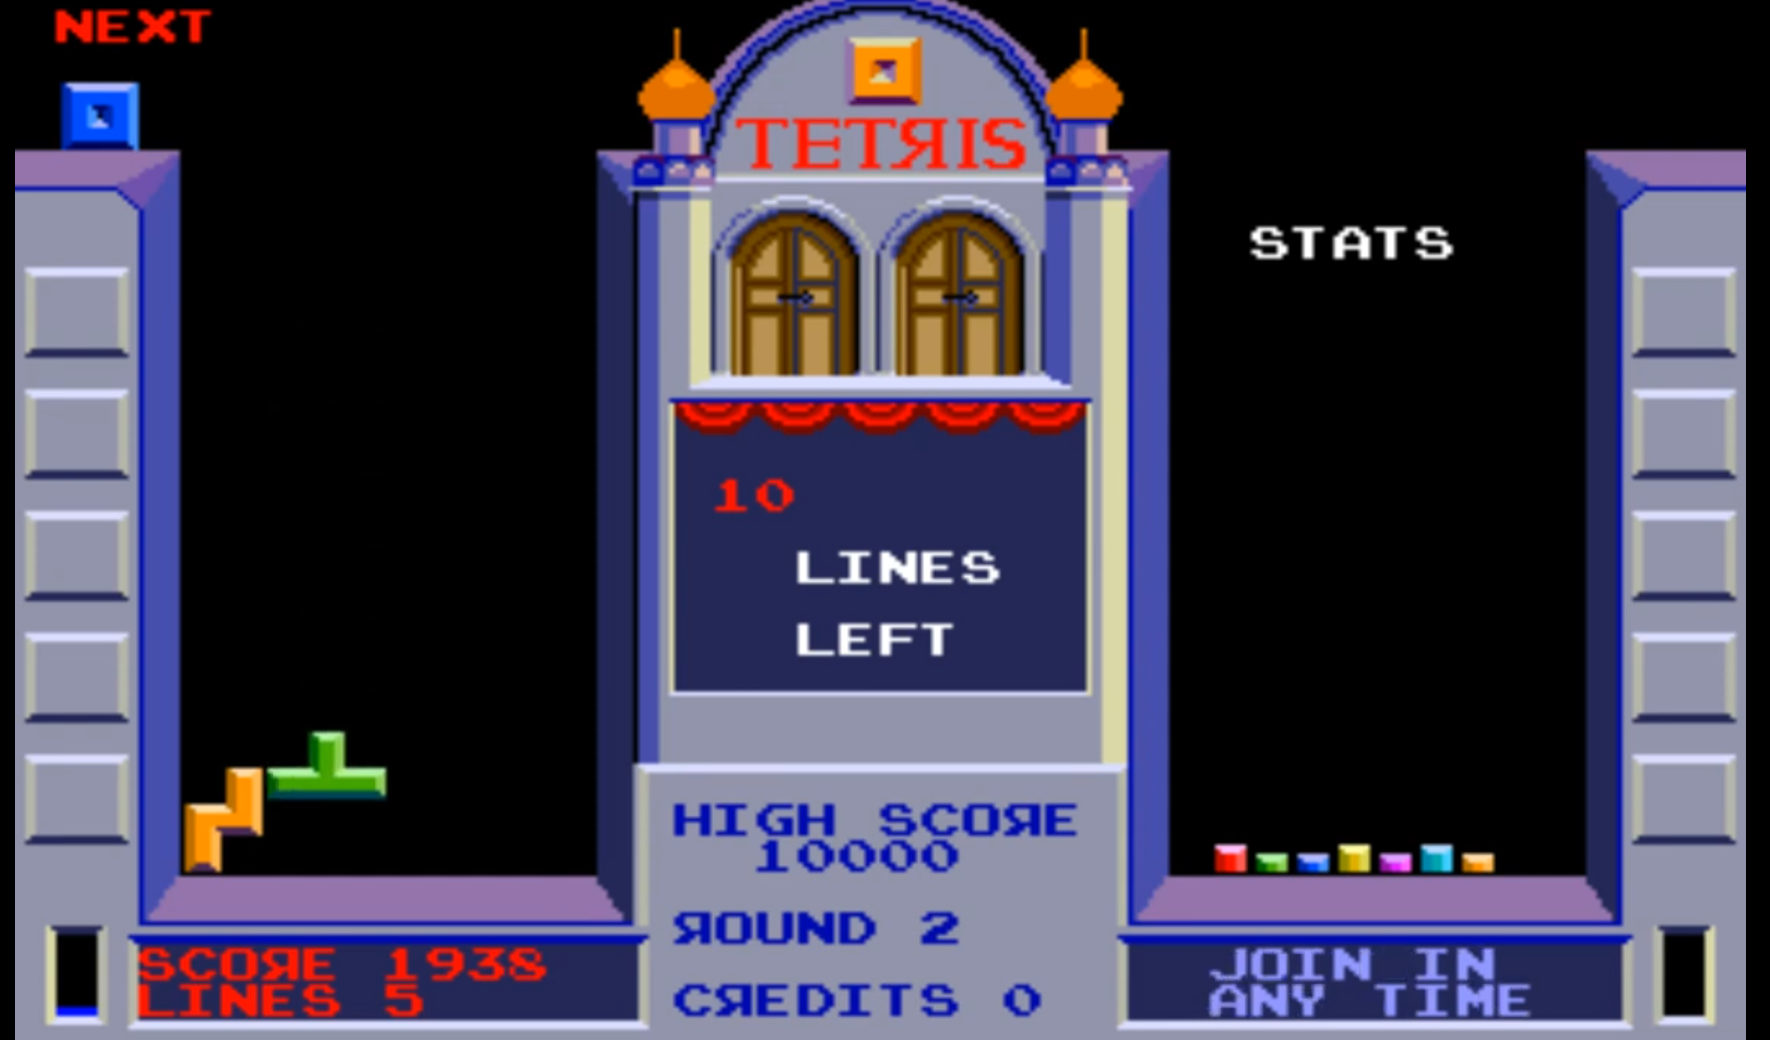
\includegraphics[width=15cm]{archivos/imagenes/tetris-1984.png}
		\caption{Tetris 1984.}
	\end{figure}
	\item Mario Bros, es un juego de tipo plataformas. Fue lanzado en 1983, en su primera versión, pero gracias al éxito que tuvo le siguió una larga saga de continuaciones del mismo y otras versiones con el mismo personaje principal y secundarios en las que el juego no trataba de lo mismo. En este juego sí que te encontrarás con personajes, has de enfrentarte a ellos, pero como el atractivo principal del juego es llegar a la meta moviéndote, la inteligencia de los mismos no requiere de ser muy compleja. Todos los personajes que aparecen tienen un comportamiento programado (también conocido como \gls{ia} diseñada), como moverse de lado a lado, salir de una tubería después de cierta cantidad de segundos, etc. Lo importante es que, aún con la presencia de enemigos, no era necesario una \gls{ia} muy desarrollada.\footnote{Para entender mejor el juego, puede visitar \url{https://www.youtube.com/watch?v=ly8DofqCuOs}}
	\begin{figure}[h]
		\centering
		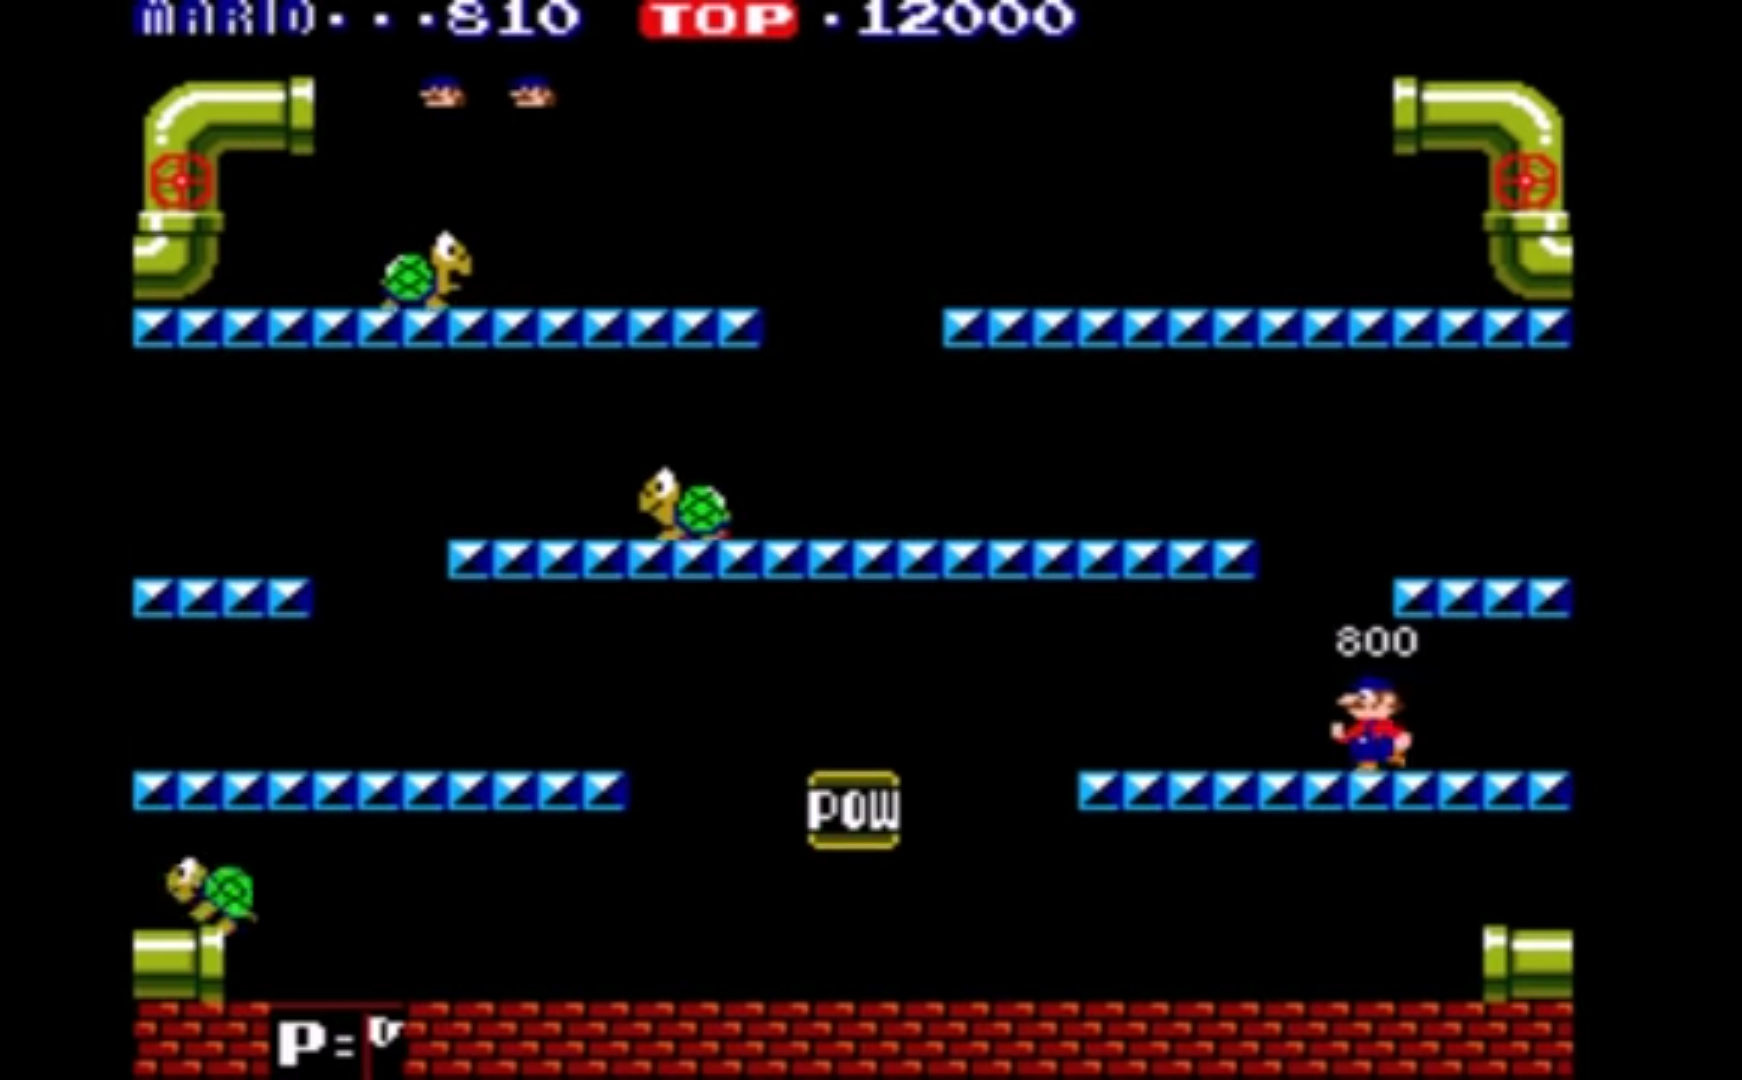
\includegraphics[width=15cm]{archivos/imagenes/mario-bros-1983.png}
		\caption{Mario Bros 1983.}
	\end{figure}
	\item Pokemon Red, Pokemon Green y Pokemon Blue. Los tres fueron lanzados en 1996, y son prácticamente iguales pero con sutiles diferencias. Estos juego son del tipo \gls{rpg}, es decir, que te introduce en la vida de un personaje, y has de jugar como si fueras tú el que toma y sufre las decisiones tomadas. A diferencia de Mario Bros, que tenías que moverte en una sola dirección y saltar, aquí te moverás en dos direcciones, y por lo tanto, los \gls{npc} también, pero estos siguen sin presentar ningún tipo de inteligencia avanzada, ya que normalmente siguen patrones en su camino que ya han sido programados, y los ataques que lanzan los Pokemon enemigos en los combates parecen ser aleatorios.\footnote{Para entender mejor el juego, puede visitar \url{https://www.youtube.com/watch?v=C034iux-EJ8}}
	\begin{figure}[h]
		\centering
		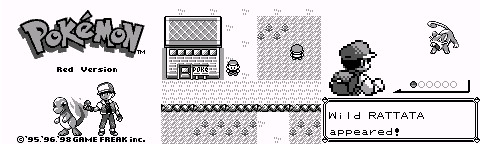
\includegraphics[width=15cm]{archivos/imagenes/pokemon-red.jpg}
		\caption[Pokemon Red.]{Pokemon Red\footnotemark.}
	\end{figure}
	\footnotetext{Imagen en la web retrospilling.no \url{https://retrospilling.no/2015/02/litt-om-pokemon/}}
	\item Left 4 Dead es un juego de supervivencia, y fue lanzado en 2008. Se trata de un juego de zombies en el cual vas con un equipo de cuatro personas, es aquí donde entra la \gls{ia}. Puedes jugar con tres amigos más, pero el juego también está hecho para jugar solo, por lo que los otros personajes requieren una inteligencia para ayudarte a completar los desafíos. No se conoce a ciencia cierta cómo está programado, pero se puede deducir que los \gls{npc} no tienen inteligencia para la búsqueda de rutas(pathfinding es el término más conocido) porque las rutas ya están definidas en el juego, pero sí cuando disparar, salvarte, etc.  mientras que los enemigos parecen comportarse siempre de la misma manera. Por lo que Left 4 Dead es el primer juego que tiene una \gls{ia} compleja de entre los que he mencionado hasta ahora.\footnote{Para entender mejor el juego, puede visitar \url{https://www.youtube.com/watch?v=oIHNW-cSGHI}}
	\begin{figure}[h]
		\centering
		
\includegraphics[width=15cm]{archivos/imagenes/Left-4-Dead.jpg}
		\caption{Left 4 Dead, primera versión.}
	\end{figure}
	\item League of Legends es un juego más actual, jugable en PC y fue lanzado en 2009. Pero además, ha sido lanzada una versión independiente para móviles en el año 2020. Este juego se trata de un \gls{moba}, en el cual te enfrentas con tus compañeros, contra otros cuatro oponentes y has de derrotar la torre principal del enemigo para ganar, teniendo como obstáculos no solo a los oponentes, sino también a minions y las propias torres que se encargan de dispararte. Podría parecer que no hay ninguna \gls{ia}, pero lo cierto es que sí que se aplica un campo que es el de la búsqueda de la ruta más rápida. Esto está presente en muchos otros juegos, y es cierto que es un campo de la \gls{ia}, pero no requiere de aprendizaje, por lo que no ha de ser entrenado con técnicas de \gls{ml} y no es necesario programar redes neuronales para el uso de la misma. Esto es usado tanto por los minions, para moverse por el mapa, como por el jugador, que se mueve haciendo clicks donde quiere ir, y no con AWSD como es típico en los videojuegos más actuales.\footnote{Para entender mejor el juego, puede visitar \url{https://www.youtube.com/watch?v=PZ2ORXhIrVU}}
	\begin{figure}[h]
		\centering
		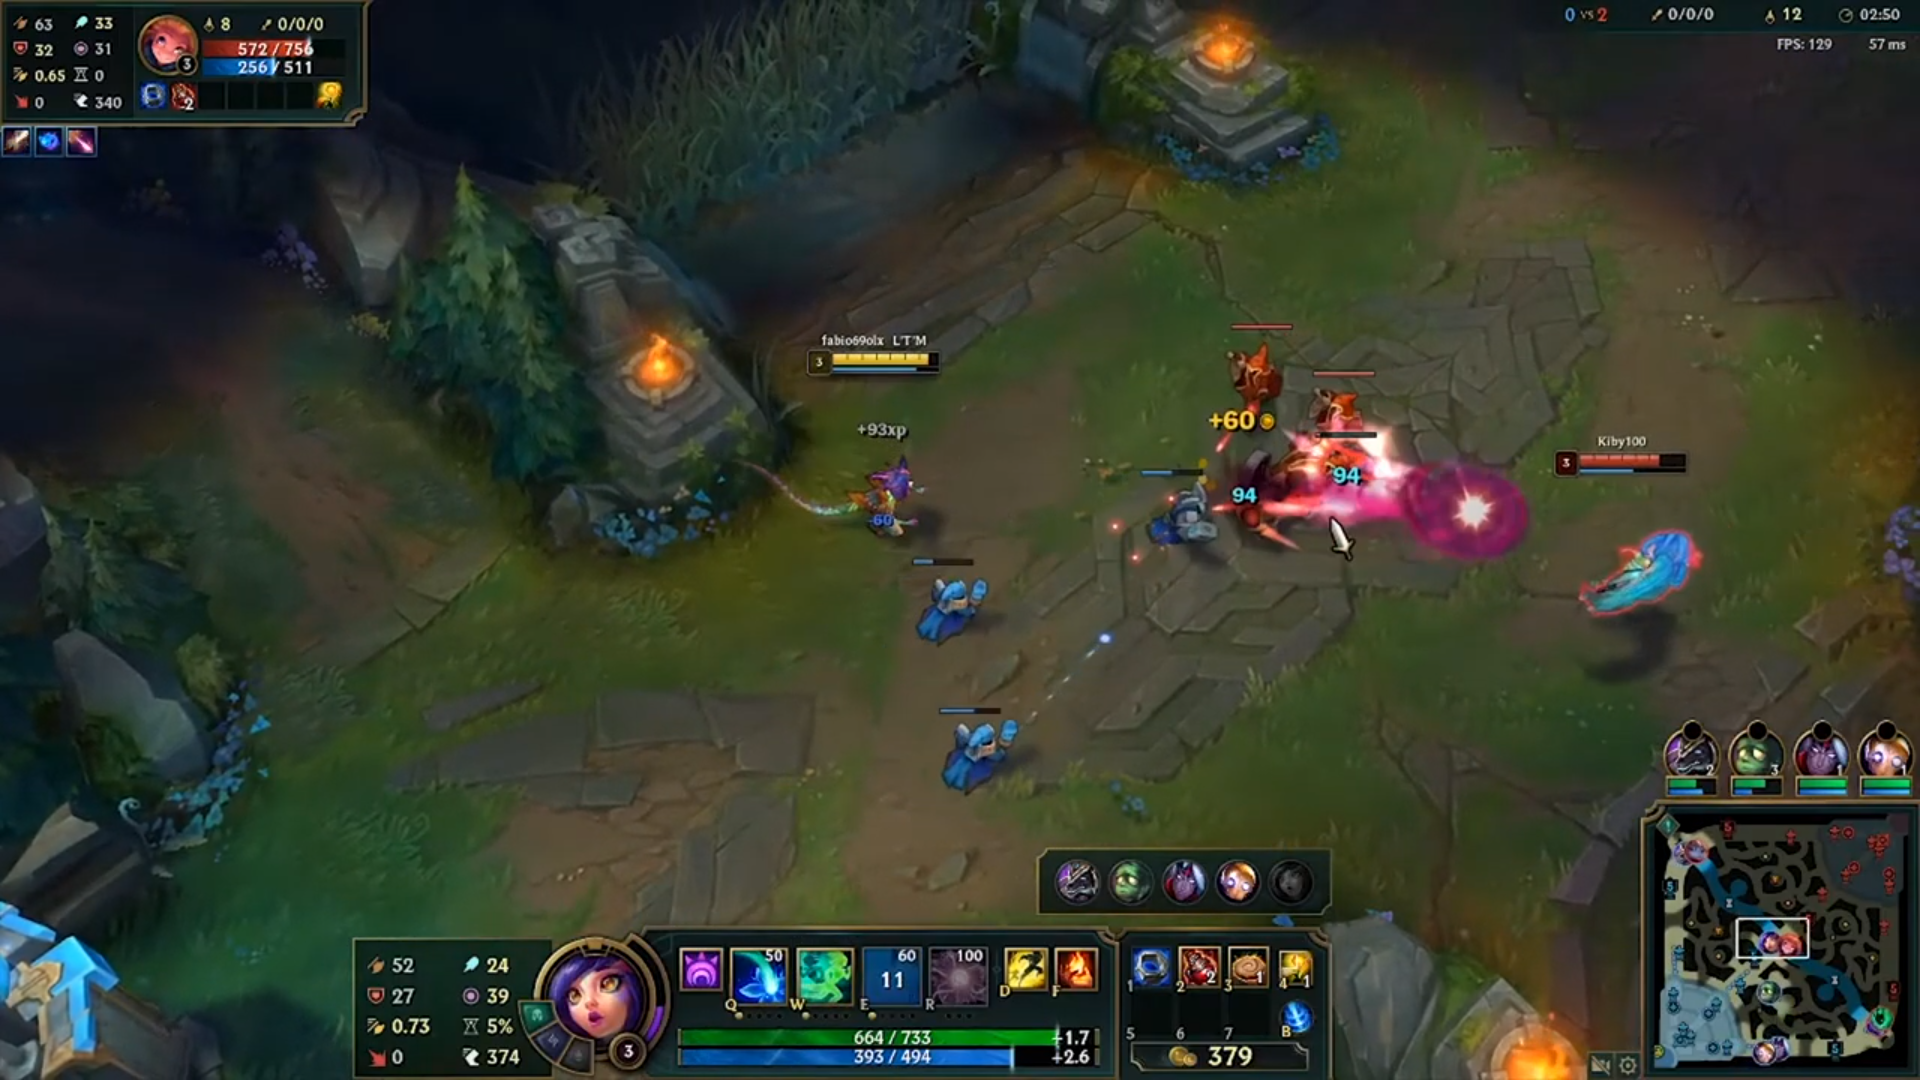
\includegraphics[width=15cm]{archivos/imagenes/league-of-legends.png}
		\caption{League of Legends.}
	\end{figure}
\end{itemize}

De todos los juegos mencionados anteriormente, no se puede saber si fueron creados utilizando un motor de videojuegos, salvo si los autores de los mismos desvelasen los detalles, pero es fácil de deducir que los más antiguos no utilizaron un motor, sino que fueron creados desde cero, pero los que tuvieron sagas reutilizarían parte del código, con lo que muchas de las partes del código las acabarían integrando en un motor, para la posterior creación de los siguientes juegos de la saga. Mientras que todos los juegos actuales utilizan un motor, debido a que ya existen motores muy buenos, y gastar el recursos del desarrollo en algo que ya existe haría perder beneficios a la empresa desarrolladora del videojuego.

\section{Motor de videojuegos}
El motor de videojuegos es el software encargado de que el desarrollador de videojuegos pueda programar estos sin tener que preocuparse por lo cómo se gestionan las entidades del juego, solo pensando en la lógica de las mecánicas, y demás aspectos del videojuego. 
\\
Después de la creación de los primeros juegos, los programadores de videojuegos se dieron cuenta de que había partes del desarrollo que se repetían. Algunas como la creación y destrucción de entidades entre otras cosas. Por eso, las empresas dedicadas a ello, comenzaron a diferenciar la parte de la creación del juego con la del motor, ya que, con un mismo motor, se podrían hacer distintos videojuegos.
\\
Pero fue en los años 90, con la creación de videojuegos en 3D donde se acuñó el termino de ``motor gráfico''. Fue debido a que en la mayoría de los casos, el motor no solo se encargaba de la gestión de entidades sino también de la renderización del juego, así que de esta forma se entendía mejor para qué servía esta pieza de software. El que se conoce como primer motor gráfico para PC fue Freescape Engine, que se utilizaba para hacer juegos de disparos en primera persona, esto es debido a que los primeros juegos en popularizarse para PC fueron de este género.
\\
Realmente los motores gráficos no solo sirven para crear juegos, así que con el tiempo, estos motores se empezaron a utilizar no solo para videojuegos, sino también para desarrollar aplicaciones que tengan que ver con simulación de la vida real, como pueden ser aplicaciones arquitectónicas, educación, simuladores para aprender a conducir, y un largo etcétera.

Actualmente, en el mundo hay muchos motores de videojuegos, algunos públicos de pago (Unreal Engine, Unity, etc.), utilizado sobretodo por desarrolladores indie, otros privados para que una empresa lo utilice o reutilice para hacer sus videojuegos, e incluso cabe mencionar Godot Engine por ser el más famoso entre los motores de libre uso, sin coste para el desarrollador. En general, el mundo de los motores es un mundo bastante maduro, aunque de vez en cuando surjan mejoras.
\\
Y con tanta oferta de motores, es obvio que estos existen porque el mundo de los videojuegos se ha ampliado, hasta tal punto que existen de todo tipo y para una gran cantidad de plataformas. En ordenadores existen plataformas de venta de videojuegos como Steam o Epic Games entre otros, donde puedes encontrar infinidad de títulos, entre los que me gustaría destacar Minecraft, Hollow Knight y Braid, demostrando que en el mundo de los videojuegos no hace falta ser enormes multinacionales para hacer juegos tremendamente entretenidos y con mecánicas originales. Mientras que en plataforma móvil, la mayoría de juegos los adquirirás en el Market Place\footnote{Un market place es una aplicación del sistema operativo desde la cual puedes encontrar y descargar otras tantas aplicaciones.} del sistema operativo que use tu móvil, y por lo general, el mercado está copado de juegos casual con los que pasar un rato, pero también hay algunas joyitas, ya que las empresas de videojuegos se han dado cuenta de que es un mercado en crecimiento, Monument Valley, Pixel Dungeon o juegos ya famosos en PC que han portado su juego a versión móvil como League of Legends, Call of Duty o Mario Kart.

En este \gls{tfg} voy a usar uno de creación propia, en base a las lecciones aprendidas en el curso de \citep{CursoMotorC++}, pero el mercado de motores de videojuegos es tan extenso que hay muchos que podrían ser usados para el proyecto. Pero como la motivación del mismo es desarrollar las tecnologías de un videojuego desde cero, me he decidido por desarrollar el mío en el lenguaje C/C++ con el uso de algunas pocas librerías externas.

\section{Videojuegos}
Fueron creados como entretenimiento, mediante el uso de un hardware que actúa como entrada en el juego los interpreta y el juego actúa según la lógica programada. Los primeros datan de los año 1952 y 1958 (Tres en raya y Tennis for Two respectivamente). Pero con el paso de los años han progresado, llegando a ser más complejos. 
\\
Con el auge de las consolas, muchas empresas surgieron y crearon videojuegos, como Nintendo con su mundialmente conocido Mario Bros, Game Freak con Pokemon, y un largo etcétera. 
\\
Después de varios años, y la creación de motores de videojuegos, la gente empezó a poder tener ordenadores en casa. Surgen distintas tecnologías como Flash Player para navegadores, con lo que alguien con conocimientos de programación podía crear su videojuego sin preocuparse del renderizado, y compartirlo con el resto de usuarios de ordenador que tuvieran esta tecnología instalada en su navegador.

Conforme fue haciéndose más grande la industria de los videojuegos, algunas empresas empezaron a comercializar su motor de videojuegos, no solo vendiéndolo a otras grandes empresas que pudieran comprarlos, sino a pequeños desarrolladores, llamados desarrolladores indie\footnote{El término proviene de desarrollador independiente, que no trabaja para una empresa sino que crea sus propios juegos.}, los cuales no pueden permitirse costes tan altos. Pero si una empresa que desarrolla el motor consigue vender licencias más baratas a una cantidad muy grande de gente, hace que también sea rentable el desarrollo de motores de videojuegos. A causa de esto, y cuando Steam permitió vender juegos a los desarrolladores indie en su plataforma, aumentó la cantidad de videojuegos en el mercado.

Otra industria que ha crecido en los últimos años de manera exponencial son los videojuegos para móvil. A pesar de que con los primeros móviles ya se podía jugar a juegos más sencillos que ya venían preinstalados, como el Snake, el verdadero auge ha sido con la popularización de los sistemas operativos Android e iOS. Estos dos sistemas operativos son los que dominan en la actualidad todo el mercado de los móviles, y vienen con un marketplace instalado, cada uno el suyo. Tanto la Play Store (de Android) como la App Store (de iOS) permiten a cualquier desarrollador subir sus propios videojuegos\footnote{Para subir cualquier aplicación a una de ellas has de cumplir unos requisitos. Ya que es un servicio centralizado, tiene que pasar unos estándares de seguridad para no ser utilizado como puerta de entrada de virus o programas no deseados.}, con lo que se expandió aún más el mercado de los videojuegos. De hecho, el mundo de los videojuegos móviles es tan popular que algunos motores de videojuegos te permiten compilar tu juego tanto para móviles como para ordenador, pudiendo de esta manera, rentabilizar aún más tu juego al abrirte a un mercado mayor, y esto ha hecho que aún más gente se anime a dedicarse a ser desarrollador.

Aunque actualmente, en el año 2021, la mayoría de juegos son construidos tanto para consola como para ordenador, por lo que con un ordenador puedes jugar casi todos, al principio se diseñaban máquinas especialmente para jugar, véase Atari 2600, NES, Game Boy, Mega Drive, Nintendo 64. Es decir, los juegos se hacían especializados para el hardware de la máquina, sin embargo, la popularización de los ordenadores domésticos hizo que cada vez haya que hacer los juegos más genéricos, y si una máquina en concreto necesita de una tecnología distinta, el motor se encarga de usarla a la hora de la compilación.

\subsection{\glsentrylong{ia}}
Cuando hablamos de \gls{ia} nos referimos a máquinas imitando comportamientos inteligentes. Esta definición es dada en 1955 con el nacimiento de la \gls{ia}. Pero si hablamos de \gls{ia} podemos estar hablando de distintos campos, ya que es un término muy genérico. Más concretamente, en este \gls{tfg} tratamos el campo del \gls{ml}.
\\
Para comprender la diferencia entre un comportamiento programado y un comportamiento aprendido me gustaría citar a Stuart J. Russell y Peter Norvig, \textit{"un agente aprende cuando su desempeño mejora con la experiencia; es decir, cuando la habilidad no estaba presente en su genotipo o rasgos de nacimiento"}.\footnote{Cita escrita en el libro \textit{Inteligencia Artificial: Un Enfoque Moderno} de los autores anteriormente mencionados.} Por lo tanto, podremos diferenciar dentro del mundo de la \gls{ia} (que es una lógica aplicada por una máquina), al \gls{ml} (que es un comportamiento, que además de ser aplicado por una máquina, ha de ser aprendido). Se hablará más en detalle sobre el \gls{ml} en el apartado \ref{importancia ml}.

La primera tecnología que permitía a una máquina tener \gls{ia} que aprendiese fue el perceptrón, presentado en 1959 por Rosenblatt. El perceptrón resuelve muy bien problemas generales, y de forma perfecta problemas que sean linealmente separables, como puede ser una puerta OR o una puerta AND, pero pronto se dieron cuenta de sus limitaciones, dado que una puerta lógica XOR no es linealmente separable, el perceptrón no funcionaba de forma correcta en estos casos. Este problema se solucionaría usando un segundo perceptrón, por lo tanto la lógica del programa depende de dos salidas, y sí que se podría separar.
\begin{figure}[h]
	\centering
	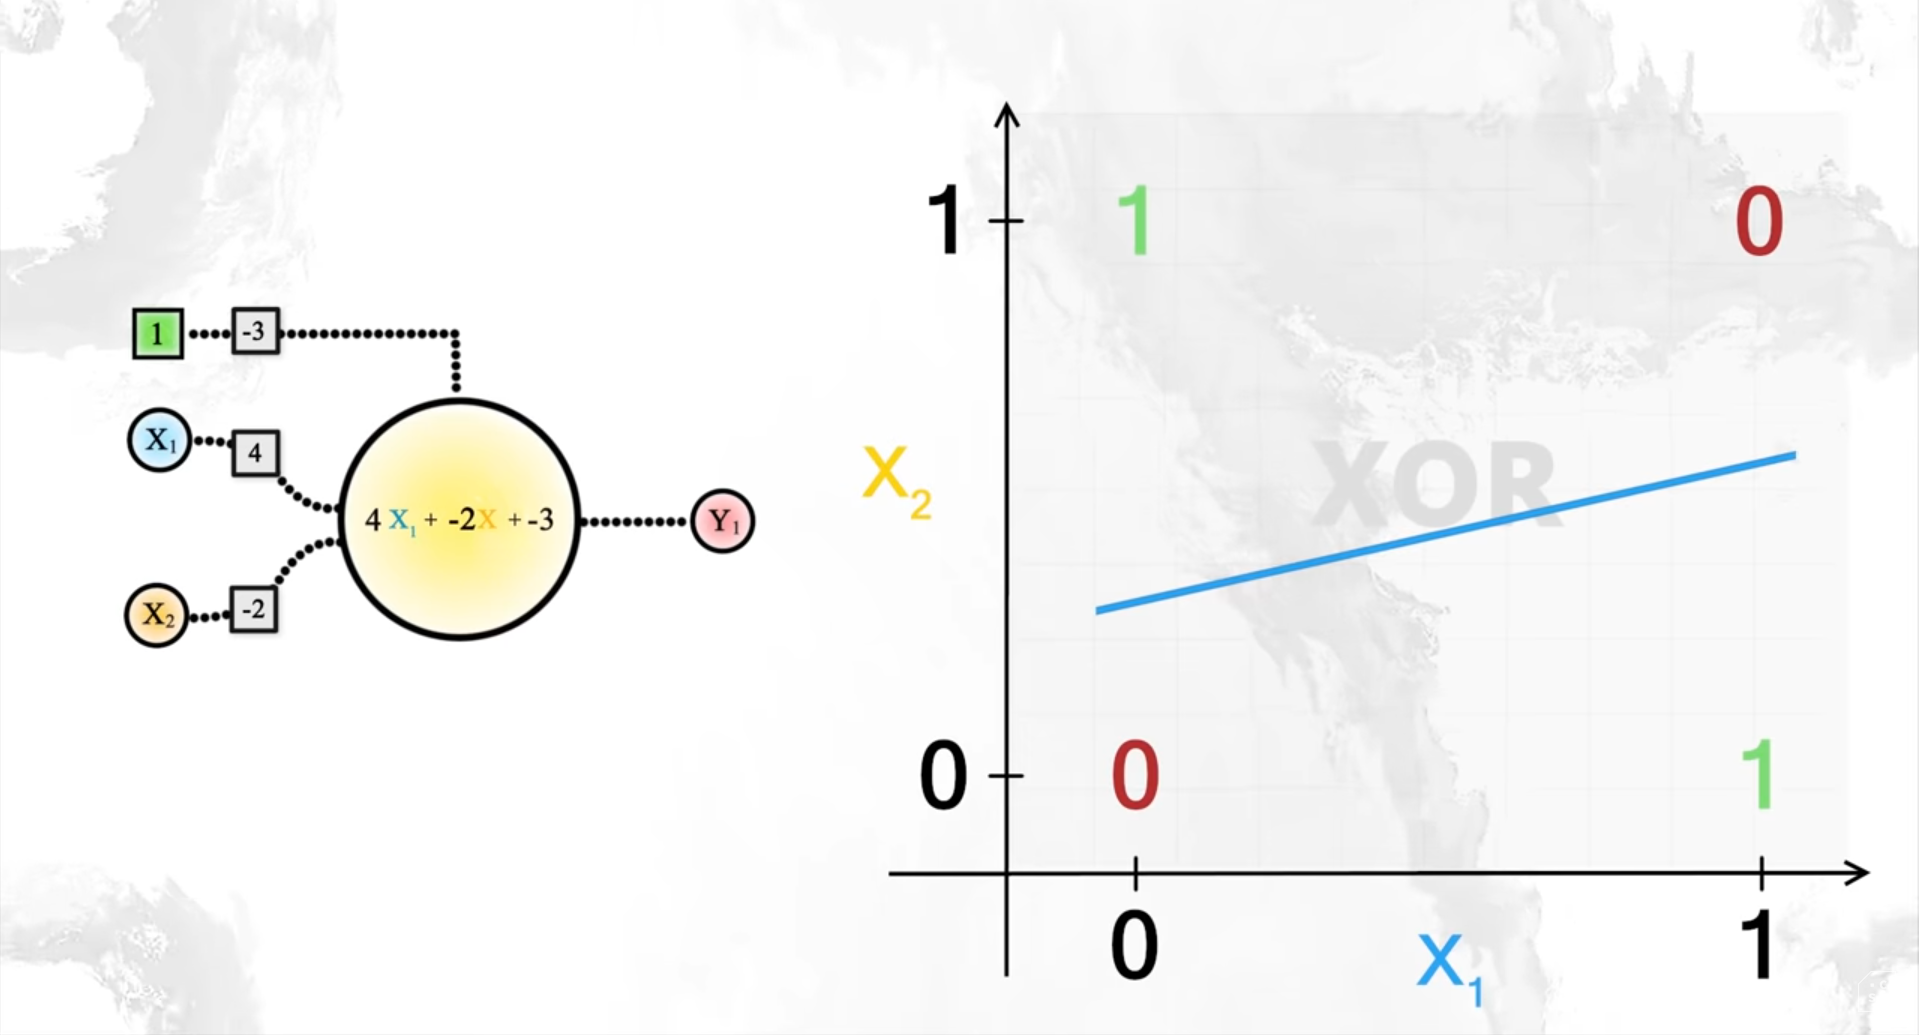
\includegraphics[width=15cm]{archivos/imagenes/problema-xor.png}
	\caption[XOR irresoluble por un solo perceptrón.]{XOR irresoluble por un solo perceptrón\footnotemark.}
	\label{XOR con un perceptron}
\end{figure}
\footnotetext{Desde el canal de YouTube de Carlos Santana \url{https://www.youtube.com/watch?v=MRIv2IwFTPg}}

Pero el perceptrón no es el único modelo dentro del mundo de la \gls{ia}, en 1940 Warren McCulloch y Walter Pitts crearon un modelo informático que se llamaba lógica umbral, esto es lo primero que se conoce sobre redes neuronales. Si bien, su lógica es parecida a la del perceptrón, tiene algunas diferencias. 

Dada la lógica del perceptrón, y resuelta la problemática de los problemas no separables linealmente, se crearon las redes de perceptrones, también llamadas \gls{mlp}. Con ellas se podían resolver problemas como el de la puerta XOR, pero pronto se dieron cuenta de sus limitaciones, y es que al final, el hecho de aplicar múltiples funciones aritméticas f(x) con sumas y multiplicaciones en cadena era equivalente a hacer una sola función aritmética f(x). Pero esto fue solucionado fácilmente cambiando la función de activación. Mientras que la función de activación de un perceptrón era una función escalonada, la función de activación de una neurona puede ser cualquier función matemática, las más comunes son la sigmoide, la ReLU, y la tangente hiperbólica. Esto es la principal diferencia entre un perceptrón y una neurona.
\\
Las limitaciones de las redes neuronales salieron a la luz después de hacer experimentos, ya que era demasiado costoso computacionalmente saber qué neurona dentro de la red neuronal había cometido el error, puesto que el método de búsqueda era por fuerza bruta, y esto supuso un gran parón en el mundo de la \gls{ia}, porque ajustar los pesos de la red manualmente era inviable para redes muy grandes y además porque el poder computacional en aquellos tiempos era más limitado.
\\
Pero en 1986 se inventó un algoritmo que era capaz de, en función de un error dado en la salida de la red neuronal, propagar el error hacia las neuronas de capas anteriores, de forma que cada una corregía su peso en la red neuronal en función de lo culpable que era en ese error. Su nombre es retropropagación, o como se le conoce por su nombre en inglés ``Backpropagation''. 

Actualmente el mundo de las \gls{ia}, aunque existen sistemas muy complejos y completamente desarrollados, es un mundo en el que constantemente recibimos nuevas noticias de un sistema que mejora al anterior, o que consigue hacer cosas nunca antes vistas. Así que podríamos decir que es menos maduro y tiene muchísimo margen de mejora aún.
\\
Algunos de los frameworks más usados para desarrollar \gls{ia} actualmente son TensorFlow y Keras entre otros, debido a su potencial y su sencillo uso, ya que no tienes que ser un experto para poder usarlas y poder programar tú mismo la \gls{ia}.

\subsection{¿Cómo resolver el problema del perceptrón?}
Sabiendo que el problema del perceptrón, que sólo podía resolver problemas linealmente separables, y que juntando varios obtenemos lo que en inglés se llama \gls{mlp} y por lo tanto, podemos resolver problemas como la XOR, pero sigue existiendo limitaciones. ¿Cuáles son estas limitaciones y por qué se dan?
\\
Para resolver estas preguntas has de entender qué es lo que hace un perceptrón gráficamente, y no de forma analítica. Como vemos en la figura \ref{XOR con un perceptron}, tenemos un perceptrón de dos entradas y una salida, pero no solo eso, sino que esto significa que el total de pesos que contiene es dos, o lo que es lo mismo, el número de parámetros libres del modelo es dos. Por lo tanto, el perceptrón es representable en una gráfica bidimensional, como lo que se conoce por una recta. Si despejamos cualquiera de las dos variables, obtendremos la ecuación de la recta:
\begin{equation}
	y = m*x + n
\end{equation}
El siguiente paso es colocar las entradas del dataset en la gráfica. Como ya habremos despejado uno de los términos, ese será el que haga de ``y'', y el otro de ``x''. Como vemos de nuevo en la figura \ref{XOR con un perceptron}, el perceptrón $4*X_1 + -2*X_2 + -3$ representado por la recta en azul, no es capaz de separar los 1s y los 0s. Mientras que en la siguiente gráfica que es la que representa los valores de una puerta AND vemos que un solo perceptrón sí que es capaz de resolver el problema.
\begin{figure}[h]
	\centering
	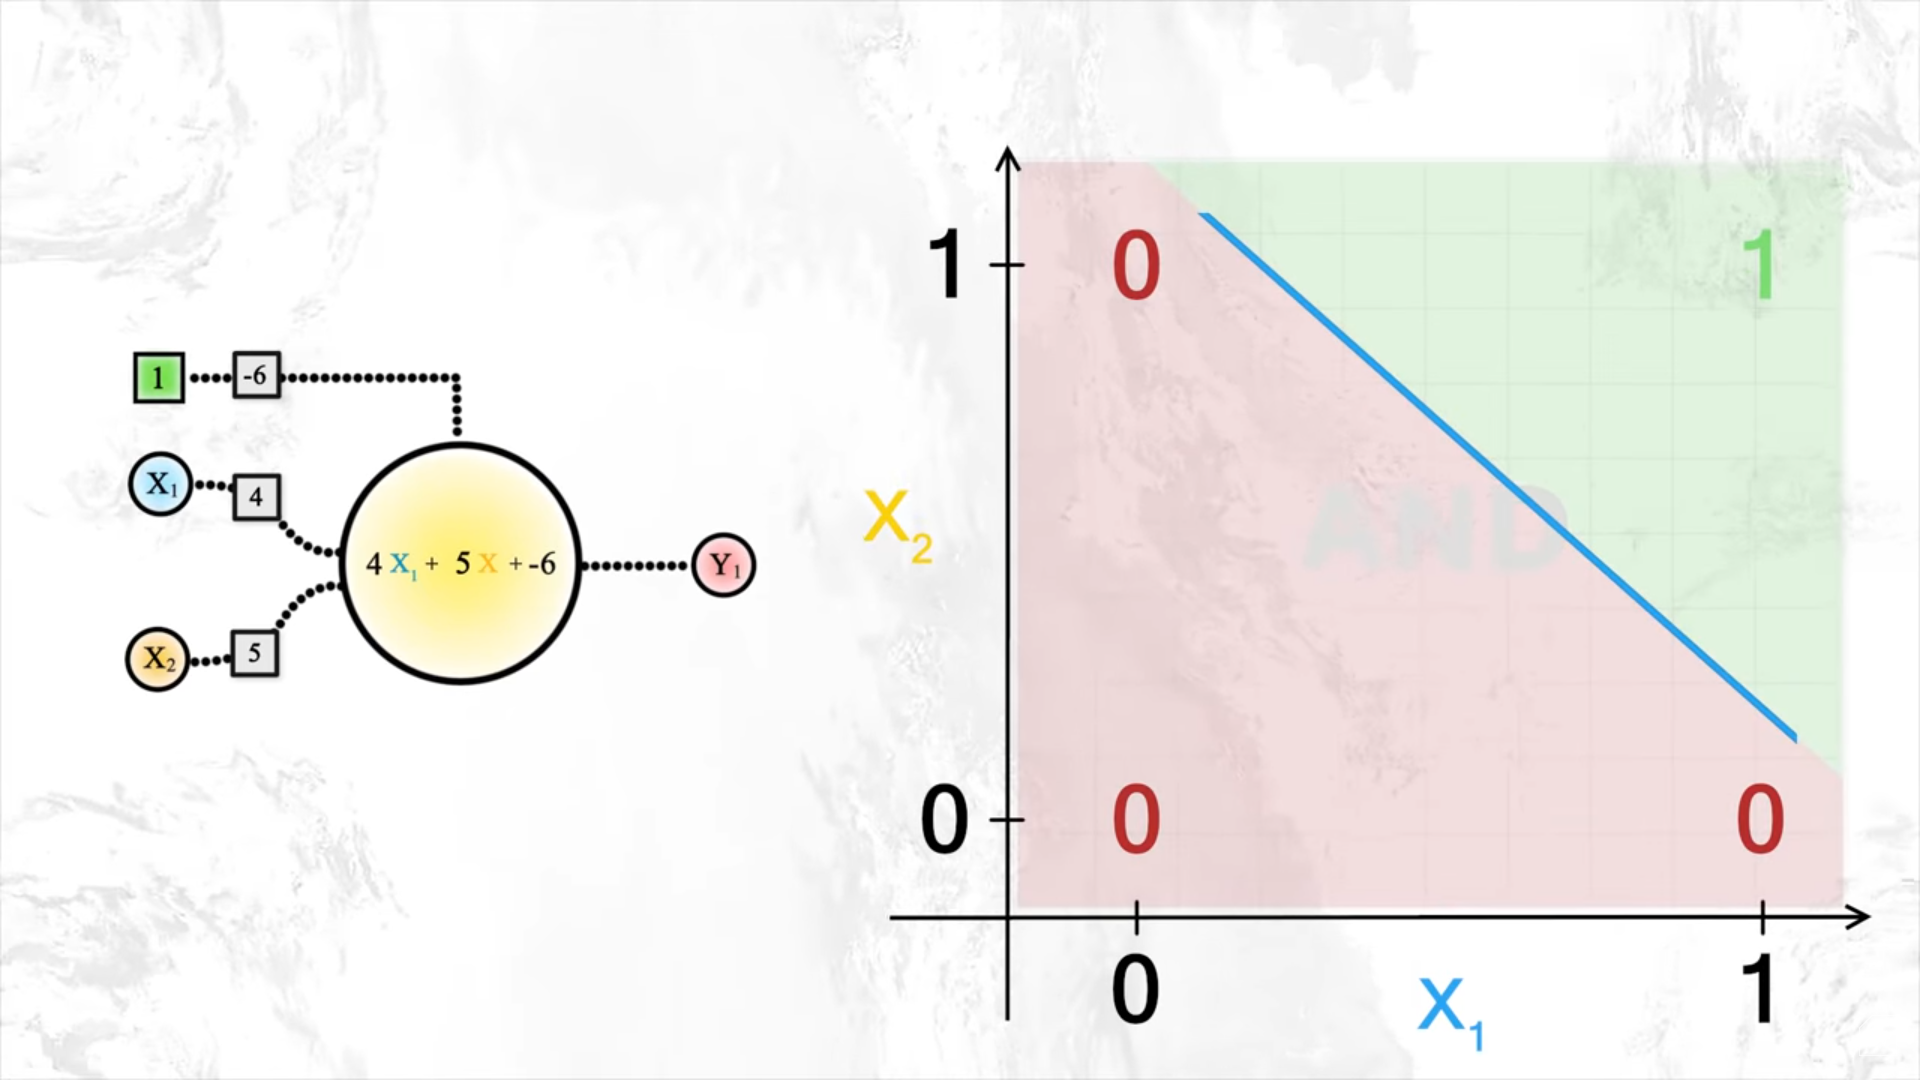
\includegraphics[width=15cm]{archivos/imagenes/perceptron-con-and.png}
	\caption[AND resuelta por un solo perceptrón.]{AND resuelta por un solo perceptrón\footnotemark.}
\end{figure}
\footnotetext{Desde el canal de YouTube de Carlos Santana \url{https://www.youtube.com/watch?v=MRIv2IwFTPg}}

Después de entender qué es un perceptrón gráficamente, una recta, es sencillo darse cuenta de que uno sólo no sería capaz de resolver el problema de la XOR, pero dos rectas sí que serían capaces de hacerlo, por eso es por lo que cobra sentido el \gls{mlp}. Pero este último también tiene sus limitaciones, que veremos en el apartado \ref{Redes Neuronales}.

\begin{figure}[h]
	\centering
	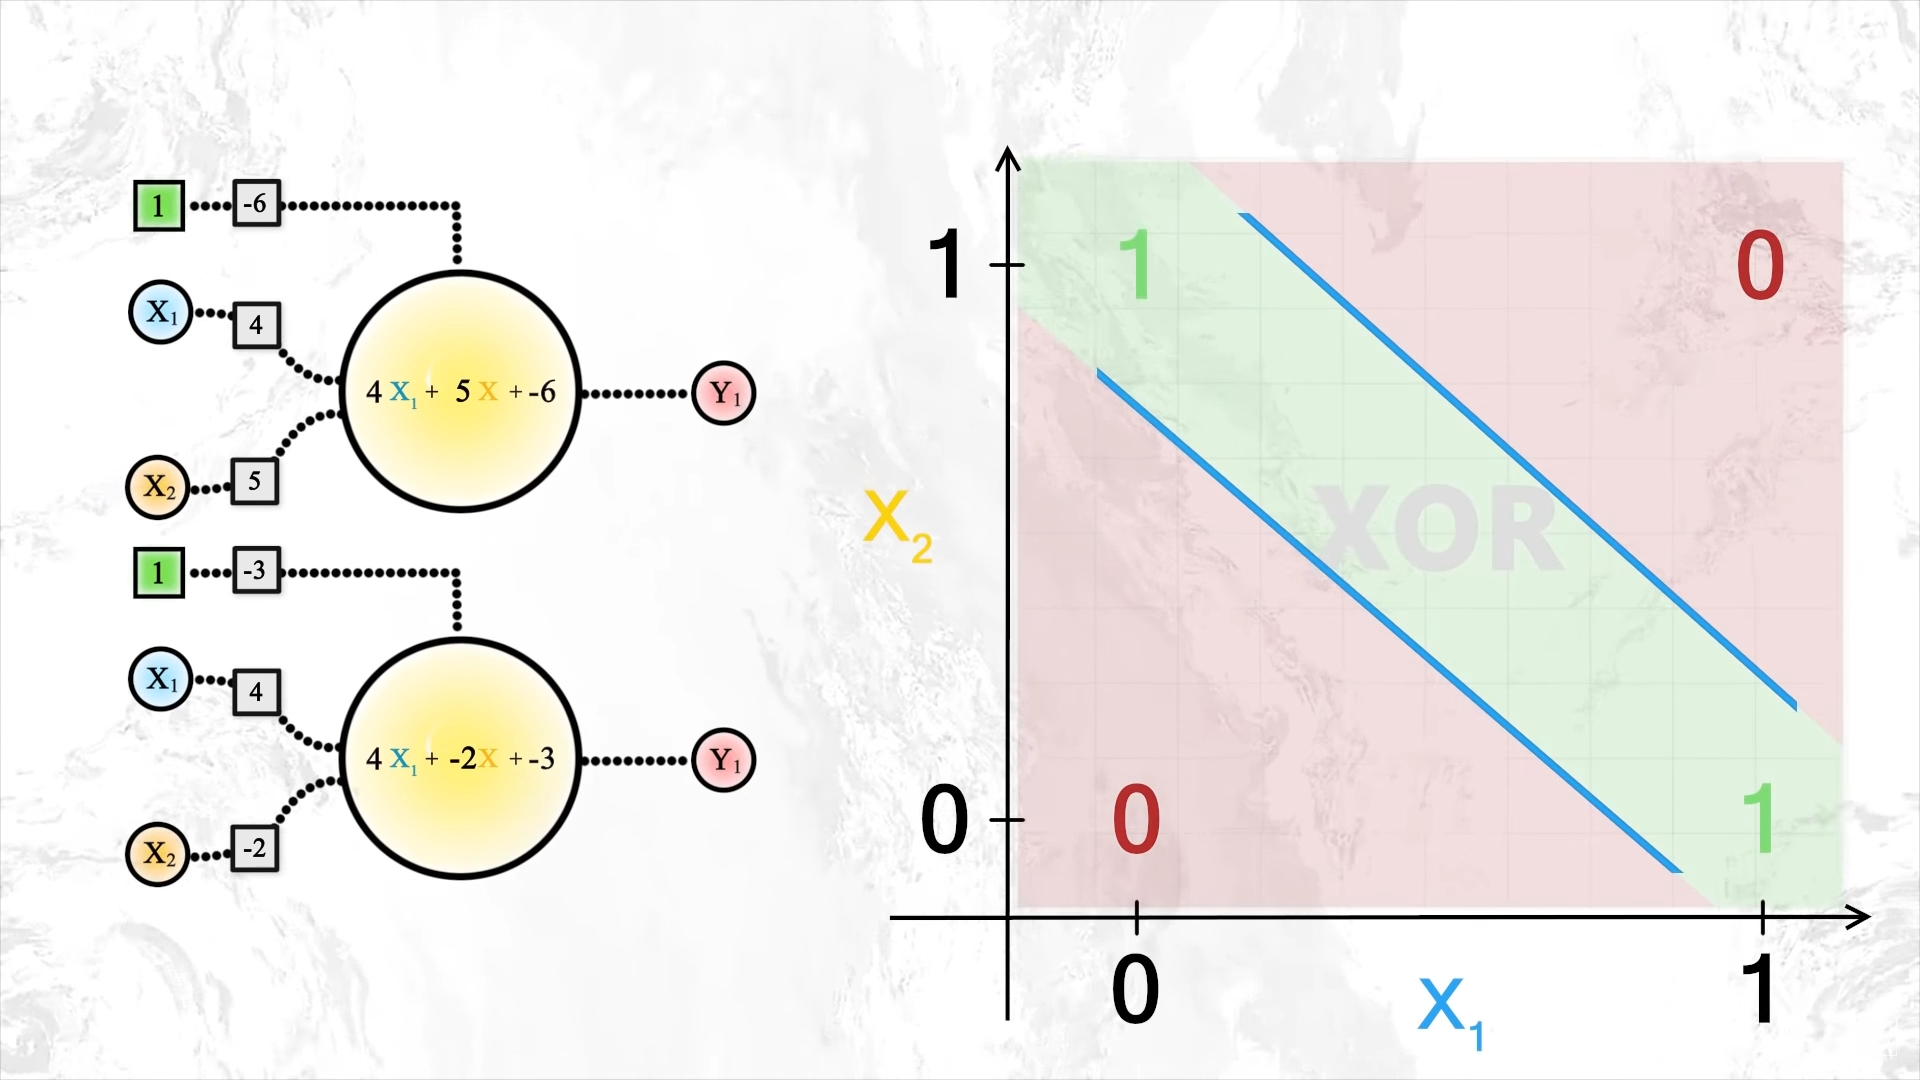
\includegraphics[width=15cm]{archivos/imagenes/problema-xor-resuelto.png}
	\caption[XOR resuelta por dos perceptrones.]{XOR resuelta por dos perceptrones\footnotemark.}
\end{figure}
\footnotetext{Desde el canal de YouTube de Carlos Santana \url{https://www.youtube.com/watch?v=MRIv2IwFTPg}}

\subsection{Importancia del \glsentrylong{ml}}
\label{importancia ml}
El \gls{ml} es un área tremendamente importante en la actualidad. No solo en el campo de los videojuegos como se desarrollará en este caso. También se aplica en distintos campos: tanto en motores de búsqueda, análisis de mercados, detección de enfermedades y muchos más. 
\\
Esto es debido a que estos problemas tienen complejidades suelen ser inasumibles con los algoritmos conocidos, porque se trata de complejidades NP-Hard, es decir, como mínimo, tan complejos como \gls{np}\footnote{Es el conjunto de problemas que pueden ser resueltos en tiempo polinómico por una máquina de Turing no determinista.}. 
\\
El \gls{ml} se encarga de resolver estos problemas, de tal manera que a partir de una pequeña parte de todo el espectro de datos que concierne al problema original \gls{np}, se consigue generalizar una o varias funciones que separan los datos de todo el espectro con el menor error posible.

Por muy avanzada que sea la \gls{ia}, todavía es necesario que la inteligencia de un humano intervenga para desarrollar un nuevo sistema enfocado en un aspecto en concreto. Esto es porque no existe una \gls{ia} capaz de programar un programa complejo, aunque sí se ha demostrado ya que existen \gls{ia} capaces de programar, como es el caso de GPT-3, que usa deep learning, un campo derivado del \gls{ml}.

De manera general, podemos decir que el verdadero potencial del \gls{ml} es la capacidad de analizar datos a la velocidad de un ordenador, y aplicar una lógica aprendida con esos datos para realizar predicciones.
\\
Sin embargo, es una tecnología con la que hay que tener mucho cuidado, debido a que se suele utilizar junto al Big Data, que es la forma en la que llamamos a recoger una gran cantidad de datos para analizarlos, ya que como estos datos no están revisados, estas máquinas inteligentes pueden verse afectadas por sesgos negativos. Como casos importantes tenemos el algoritmo de detección de fotos de Google, que identificaba a algunas personas negras como gorilas, o el bot de Twitter de Microsoft, que aprendió comportamientos racistas y machistas en base a estudiar el comportamiento de esta red. 

\subsection{Tipos de \glsentrylong{ml} }
La \gls{ia} es el nombre que se utiliza para englobar todos los campos donde una máquina se comporta de manera inteligente, por lo tanto, hay que concretar más. El tema que se trata en este \gls{tfg} es el \gls{ml}, que busca dotar a las máquinas de la capacidad de aprendizaje, mediante el análisis de datos empíricos de una situación en la que se pretende predecir el resultado de un dato que no está presente dentro de esa muestra, y por supuesto, predecir al mismo tiempo los que sí lo están. 
\\
La parte común que converge en todos los tipos de aprendizaje es la siguiente: la máquina genera una función aleatoria, y esta función produce una salida en base a los datos de entrada que le han sido suministrados. Esta salida será, en la mayoría de los casos, errónea (dado que la función se ha generado de manera totalmente aleatoria), y no se parecerá en nada a lo que queremos que aprenda, así que según la forma de analizar y corregir este error de salida, se distinguen varios tipos de aprendizaje, los más comunes son:
\begin{description}
	\item[Supervisado:]  Los datos de entrada son proporcionados por el usuario que quiere entrenar al agente. Una vez obtenida la salida, comparamos esta salida real con la salida esperada, que realmente era la que debía haber generado, para obtener el error. Este tipo de entrenamiento se utiliza principalmente en tareas de etiquetado, como ejemplo más común tenemos la clasificación de un número escrito a mano, es decir, que un humano escriba un ocho y el agente entienda que es un ocho.
	\item[No supervisado:] A diferencia del anterior, no proporcionaremos datos de salida. Sirve para aprender a clasificar datos, según los patrones encontrados por el agente. En el ejemplo anterior, de clasificación de números, el agente podría identificar que dos números se parecen entre sí, pero no qué número es. La principal ventaja es que al no tener que proporcionar una salida, no es necesario que un humano etiquete los datos, así que es más sencillo obtener una gran cantidad de datos.
	\item[Reforzado:] A diferencia de los dos anteriores, sólo tenemos que indicar al agente cuál es el objetivo a conseguir, indicando qué acciones reportarán estímulos positivos para él, y cuáles estímulos negativos. No se proporcionan datos de entrada ni de salida, sino que los datos de entrada los obtiene probando acciones al azar en el medio, y la salida es la respuesta, el estímulo negativo o positivo.  Este tipo de aprendizaje es el más utilizado en videojuegos, ya que como son programas informáticos, es muy fácil simular una partida una cantidad muy grande de veces, sin embargo, el hecho de que el agente haya tomado una decisión correcta en ocasiones es muy difícil de determinar, así que se usan estímulos positivos como conseguir monedas o negativos como chocarse con una pared.
\end{description}

La unidad más básica de aprendizaje en el \gls{ml} es el perceptrón. Está inspirado en las neuronas del cuerpo humano, que reciben un impulso eléctrico desde varias entradas y deciden una salida booleana que es si continuar trasmitiendo la electricidad o no. 
Un perceptrón realmente, es lo mismo que una neurona, pero con una función de activación escalonada. Suma los valores de entrada, multiplicado por un peso previamente establecido, si supera un umbral dará un resultado, y si no lo supera, otro, por ejemplo: verdadero o falso, 1 o -1, etc.

\begin{figure}[h]
	\centering
	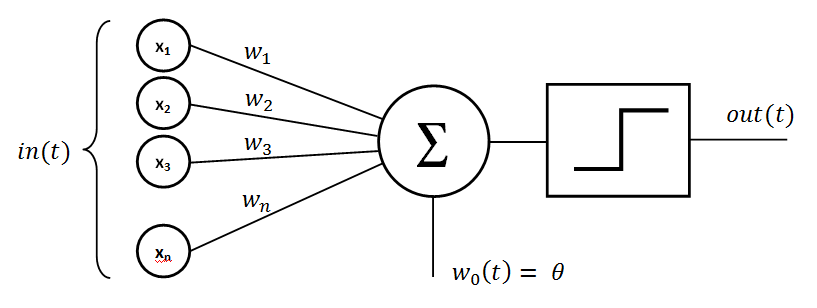
\includegraphics[width=15cm]{archivos/imagenes/perceptron.png}
	\caption[Perceptrón con entradas, pesos, y una salida escalonada.]{Perceptrón con entradas, pesos, y una salida escalonada\footnotemark.}
	\label{perceptron}
\end{figure}
\footnotetext{Puedes encontrar la imagen de de wikimedia.org en  \url{https://commons.wikimedia.org/wiki/File:Perceptron_moj.png}}                  

Ha sido demostrado mediante estudios empírico-analíticos y teóricos, que con un correcto entrenamiento del perceptrón, evitando el overfitting\footnote{El overfitting surge tras entrenar una red muy compleja con los mismos datos muchas iteraciones, de esta manera la red aprende el ruido de la muestra, y no es capaz de responder bien fuera de los datos de muestra.}, y proporcionando una cantidad suficiente de datos, que un solo perceptrón es capaz de separar los datos de cualquier problema que sea linealmente separable. Pudiendo entonces, mediante la sencilla implementación de un perceptrón, predecir patrones en cualquier campo con las condiciones mencionadas.

\section{Redes neuronales}
\label{Redes Neuronales}
Como ya hemos mencionado anteriormente, el \gls{mlp} no es capaz de resolver todo tipo de problemas. Gráficamente es fácil de entender que si el dataset del problema no es separable por rectas, el \gls{mlp} no resolverá el problema. Analíticamente se explica de la siguiente manera: cada perceptrón se entiende como un polinomio, es un sumatorio de cada peso multiplicado por cada entrada, y la suma de polinomios se puede simplificar fácilmente como un solo polinomio. Por eso es que descubrieron que usando una función de activación, esto se solucionaba, ya que gráficamente la función ya no será una recta, y analíticamente no se podrá simplificar a un solo polinomio.
Existen muchas funciones de activación, entre ellas cabe mencionar a las más usadas: la sigmoide \ref{Funcion sigmoide}, la tangente hiperbólica \ref{Funcion tangente hiperbolica}, y la ReLU \ref{Funcion ReLU}

\begin{equation}
	\label{Funcion sigmoide}
	f(x) =  \frac{\mathrm{1} }{\mathrm{1} + e^{-x} }
\end{equation}
\begin{equation}
	\label{Funcion tangente hiperbolica}
	f(x) =  \frac{\mathrm{2} }{\mathrm{1} + e^{-2x} }  - 1
\end{equation}
\begin{equation}
	\label{Funcion ReLU}
	f(x)= \left\{ \begin{array}{lcc}
		0 &   si  & x < 0 \\
		\\ x &  si  & x \geq 0
	\end{array}
	\right.
\end{equation}

Esta es la principal diferencia entre una red neuronal y una \gls{mlp}, y una diferencia que hace que la \gls{ia} se haya podido extender más aún para la resolución de problemas. Algunos de estos no tienen una resolución viable debido a que la complejidad computacional del algoritmo es extremadamente alta, otros porque ni siquiera se conoce o no se puede desarrollar un algoritmo que resuelva el problema. 
\\
Pero después de entender esta maravillosa forma de resolver casi cualquier problema surge otra cuestión, ¿cómo ajustamos los pesos de la red? Si una persona tiene que encargarse de hacerlo por fuerza bruta, sería capaz para problemas pequeños, pero cuantos más parámetros libres tenga la red, más inviable será el entrenamiento de este, ya que el tiempo que empleará entrenando crecerá exponencialmente.
\\
Por esto es que se comenzó a pensar en formas de entrenamiento alternativas, por ejemplo las redes generativas \gls{gan}, que trata de dos redes, una la cuál vamos a entrenar para resolver el problema, y otra la cuál se va a encargar de evaluar si el trabajo ha sido bien hecho. Pero la forma de entrenamiento que desarrollaré en este \gls{tfg} es el ``Backpropagation''.

\subsection{Backpropagation}
\label{marco teorico backpropagation}
Como su nombre indica, trata de propagar el error cometido en una muestra desde el final hasta el principio, es decir, hacia atrás. En el entrenamiento supervisado, conocemos el resultado que debería obtener la red, por lo tanto si probamos con una entrada, sabremos cuánto error ha cometido, y según cuánta culpa de ese error haya tenido una de las neuronas, se corregirá sus pesos de entrada más o menos.
El ``Backpropagation'' es un gran hito en la historia de la \gls{ia} ya que, anterior a esto sólo existía la corrección por fuerza bruta, es decir, medir cuánta culpa tenía una neurona del fallo implicaba mirar qué error habían cometido las neuronas posteriores a ella. Por lo que continuaba siendo un problema de complejidad computacional exponencial inviable, sobretodo teniendo en cuenta que los recursos eran más limitados.
¿De qué trata este algoritmo que simplifica tanto el aprendizaje? El algoritmo se apoya en el descenso del gradiente que es otro algoritmo que se basa en que, para encontrar un mínimo relativo en una función haremos la derivada de esta, la derivada nos aporta la pendiente en el punto, y si le restamos la pendiente a nuestra función nos iremos aproximando cada vez más a un mínimo relativo. Pero seguimos teniendo el problema de tener que hacer los cálculos para esa neurona, y las siguientes en la red.
\\
Los ingenieros se dieron cuenta de que en la corrección durante el entrenamiento había un factor que se repetía, a este lo llamaron como la letra griega delta ($\delta$), ya que en matemáticas esta letra representa el diferencia o cambio. Por lo que para aplicar la corrección a la neurona sólo tendrías que acumular los delta de las neuronas posteriores. 

El mayor problema de este es entender cómo funciona teóricamente este, ya que en código no es muy complicado de hacer una vez entiendes los índices que componen el algoritmo. Para saber cómo se implementa el, he desarrollado un esquema que puedes ver en la figura \ref{Algoritmo de backpropagation}.
\begin{figure}[h]
	\centering
	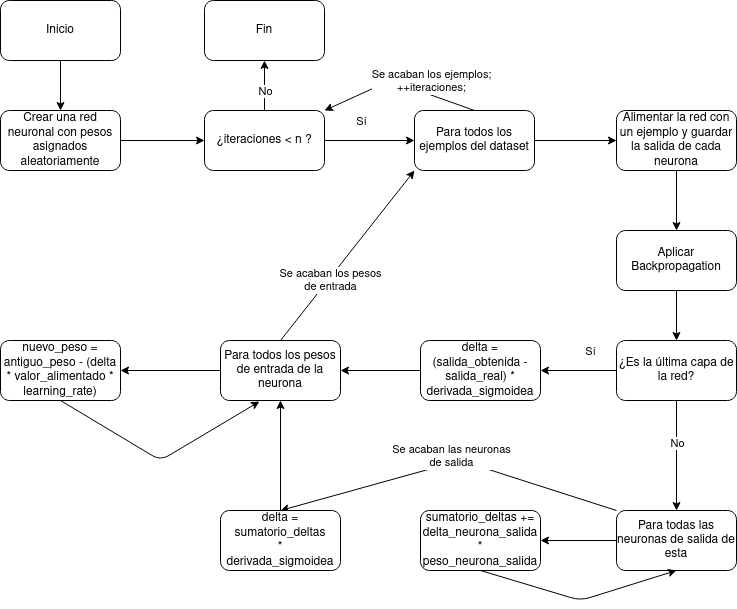
\includegraphics[width=15cm]{archivos/imagenes/Algoritmo-de-backpropagation.png}
	\caption{Algoritmo de backpropagation.}
	\label{Algoritmo de backpropagation}
\end{figure}

Y aunque parece fácil de entender viéndolo de una forma esquemática, el problema está cuando has de saber a qué índice corresponde cada fórmula en el código. Lo que haremos será escoger un ejemplo del dataset. Para cada peso de entrada (j), de cada neurona (i), de cada capa (l), vamos a aplicar la fórmula \ref{eq:descenso del gradiente} Es decir, aplica el descenso del gradiente.
\begin{subequations}
	\begin{eqnarray}
		w_{ij}^{(l)} = w_{ij}^{(l)} - \alpha*\nabla E(w_{ij}^{(l)}) \label{eq:descenso del gradiente} \\
		\nabla E(w_{ij}^{(l)}) =  \frac{\delta E(w_{ij}^{(l)})}{\delta w_{ij}^{(l)}} \label{eq:derivada parcial}
	\end{eqnarray}
\end{subequations}
El alpha que aparece, que todavía no he comentado, es el factor de aprendizaje, que hará que el descenso del gradiente sea más rápido pero más errático si es más grande, y más lento pero preciso si es más pequeño. Y la fórmula \ref{eq:derivada parcial} representa el gradiente de la función de error, es decir, en este caso la derivada parcial respecto al peso j de la neurona i.

La función de error que estoy usando en Backpropagation es el error cuadrático, es decir, la media de la suma de los cuadrados en la fórmula \ref{Error cuadratico}. Siendo $h(x)_n$ el resultado de la red neuronal para una entrada x, $y_n$ el resultado real que debería haber obtenido, y N el número total de ejemplos. Cabe destacar que el superíndice es una ele mayúscula debido a que esto connota que la capa de la que hablamos es la última.
\begin{equation}
	\label{Error cuadratico}
	E(w_{ij}^{(L)}) = \frac{1}{N}\sum_{n=0}^N(h(x)_n - y_n)^2
\end{equation}

Pero ahora queremos calcular el gradiente del error, y para eso necesitamos saber qué es lo que vale la función \ref{eq:derivada parcial}. Para eso usaremos la regla de la cadena. Pero antes de ponernos con la fórmula, hay que entender qué significa cada símbolo. 

\begin{figure}[H]
	\centering
	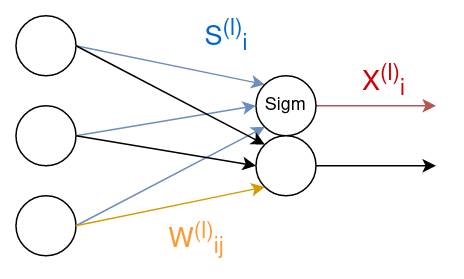
\includegraphics[width=15cm]{archivos/imagenes/Red-neuronal-simbolos.png}
	\caption{Símbolos de una red neuronal.}
	\label{fig:symb neural net}
\end{figure}

Como se puede apreciar en la figura \ref{fig:symb neural net}, la w con sus índices se refiere al peso j de una neurona i de la capa l. La S  con sus índices se refiere a la señal (sumatorio de cada entrada por cada peso) de la neurona i en la capa l. Sigm se refiere a la función de activación, la sigmoidea en este caso. Y por último x con sus índices se refiere a la salida de la neurona i (la ele minúscula indica la capa, si quisiéramos la salida de la capa anterior, que es lo que nos interesa, usaremos l-1) después de pasar por la función de activación, si fuese la capa l sería la salida de la neurona anterior.
\\
Una vez entendido cada símbolo, podemos entender la regla de la cadena que aplicamos en la fórmula \ref{Chain rule signal}. Gracias a esta regla obtenemos algo más sencillo de calcular, que es la derivada de la señal respecto al peso, mucho más sencillo de calcular como vemos en la fórmula \ref{Derivada de la señal respecto al peso}. Y a la derivada del error respecto a la señal, es a lo que llamaremos delta, que como expliqué en el marco teórico, es lo que se acumula en todas las capas, y por lo tanto lo que nos va a interesar almacenar.
\begin{subequations}
	\begin{eqnarray}
		\nabla E(w_{ij}^{(l)}) =  \frac{\delta E(w_{ij}^{(l)})}{\delta w_{ij}^{(l)}} = \frac{\delta E(w_{ij}^{(l)})}{\delta w_{ij}^{(l)}} * \frac{\delta S_{i}^{(l)}}{\delta S_{i}^{(l)}} = \frac{\delta E(w_{ij}^{(l)})}{\delta S_{i}^{(l)}} * \frac{\delta S_{i}^{(l)}}{\delta w_{ij}^{(l)}} \label{Chain rule signal} \\
		\frac{\delta S_{i}^{(l)}}{\delta w_{ij}^{(l)}} = \frac{\delta (x_{i}^{(l-1)}*w_{ij}^{(l)}) }{\delta w_{ij}^{(l)}} = x_{i}^{(l-1)} \label{Derivada de la señal respecto al peso}
	\end{eqnarray}
\end{subequations}

Pero todavía no sabemos lo que vale delta, así que volvemos a aplicar la regla de la cadena \ref{Chain rule delta}. Lo que conseguimos es obtener la derivada de la salida de la neurona después de aplicar la función de activación, respecto al sumatorio de cada entrada de la neurona por cada peso, esto es lo mismo que la derivada de la función de activación en la señal \ref{Derivada de la salida respecto a la entrada}. Y ahora ya sí que podemos obtener la derivada de la función de error respecto a la salida de la neurona \ref{Derivada de la salida de la red respecto a la salida real}.
\begin{subequations}
	\begin{eqnarray}
		\frac{\delta E(w_{ij}^{(l)})}{\delta S_{i}^{(l)}} = \frac{\delta E(w_{ij}^{(l)})}{\delta S_{i}^{(l)}} * \frac{\delta x_{i}^{(l)}}{\delta x_{i}^{(l)}} = \frac{\delta E(w_{ij}^{(l)})}{\delta x_{i}^{(l)}} * \frac{\delta x_{i}^{(l)}}{\delta S_{i}^{(l)}} \label{Chain rule delta} \\
		\frac{\delta x_{i}^{(l)}}{\delta S_{i}^{(l)}} = Sigm'(S_{i}^{(l)}) = Sigm(S_{i}^{(l)}) * (1 - Sigm(S_{i}^{(l)})) \label{Derivada de la salida respecto a la entrada} \\
		\frac{\delta E(w_{ij}^{(l)})}{\delta x_{i}^{(l)}} = \frac{\delta (h(x) - y)^2}{\delta x_{i}^{(l)}} = \frac{\delta (x_{i}^{(l)} - y_{i})^2}{\delta x_{i}^{(l)}} = 2 * (x_{i}^{(l)} - y_{i}) \label{Derivada de la salida de la red respecto a la salida real}
	\end{eqnarray}
\end{subequations}

Por lo tanto podemos concluir que el cálculo de delta, cuando estamos en la última capa L (ele mayúscula), es la fórmula \ref{Delta en la ultima capa}. Y que el gradiente para la última capa será \ref{Gradiente para las neuronas de la ultima capa}.
\begin{subequations}
	\begin{eqnarray}
		\delta_{i}^{(L)} = 2 * (x_{i}^{(L)} - y_{i}) * Sigm(S_{i}^{(L)}) * (1 - Sigm(S_{i}^{(L)})) \label{Delta en la ultima capa} \\
		\nabla E(w_{ij}^{(l)}) = \delta_{i}^{(L)}  * x_{i}^{(L-1)} \label{Gradiente para las neuronas de la ultima capa}
	\end{eqnarray}
\end{subequations}

Pero nos faltaría calcular el gradiente para las capas anteriores a la última. Como he mencionado antes, la virtud de Backpropagation\todo{DUDA URGENTE: menciono muchas veces backpropagation en la memoria, pero no sé si hacerlo en cursiva, entre comillas, con la B mayúscula...etc} es que vamos acumulando delta porque se propaga desde el final hasta el principio. Sólo tenemos que seguir la fórmula \ref{Chain rule signal}, es decir, multiplicar el nuevo delta (que todavía no conocemos y habremos de calcular) por la entrada que corresponde a ese peso. 
\\
Por lo tanto, ya sabemos cuál es la entrada de la señal  de entrada de la neurona que corresponde a ese peso \ref{Derivada de la señal respecto al peso}, y calcular el nuevo delta, usando la regla de la cadena, y teniendo en cuenta el delta de la capa posterior, sería: la derivada de la función de activación en la señal de entrada, por el delta de la neurona de salida, por el peso que conecta esa neurona con la neurona de salida \ref{Delta en el resto de capas}. 
\\
Para entender mejor de forma visual cómo se calcula el delta de la capa l, puedes ver la figura \ref{Delta en la capa l}. Se observa como, en este caso hay dos neuronas de salida que han tenido un error, acumulado en su delta, cada delta es multiplicado por el peso que le une a esa neurona porque si el peso es mayor, significa que tendrá más culpa del error, y también se aprecia que sigue apareciendo la señal de entrada de la neurona y la derivada de la sigmoidea, porque también han afectado al error y hay que tenerlo en cuenta para el nuevo delta.
\begin{subequations}
	\begin{eqnarray}
		\delta_{i}^{(l)} = Sigm'(S_{i}^{(l)}) * \sum_{j=0}^{n} \delta_{ij}^{(l+1)} * w_{ij}^{(l+1)} \label{Delta en el resto de capas} \\
		\nabla E(w_{ij}^{(l)}) = \delta_{i}^{(l)}  * x_{i}^{(l-1)} \label{Gradiente para las neuronas del resto de capas}
	\end{eqnarray}
\end{subequations}

\begin{figure}[H]
	\centering
	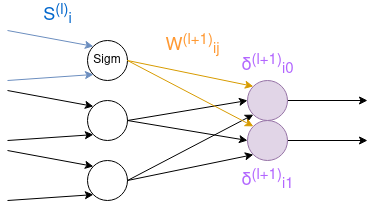
\includegraphics[width=15cm]{archivos/imagenes/Calculo-del-delta-en-la-capa-l.png}
	\caption{Cálculo de delta en la capa l $\neq$ L}
	\label{Delta en la capa l}
\end{figure}

Haremos esta operación para cada peso de cada neurona de esta capa, a ese peso le aplicaremos el gradiente como en la fórmula \ref{eq:descenso del gradiente}, y avanzaremos hacia la capa de atrás hasta que no queden más capas.

Para ver las ventajas de backpropagation de forma empírica respecto al algoritmo aleatorio, ir al apartado de resultados (\ref{resultados}).

\subsection{Dimensión Vapnik-Chervonenkis}
Ahora sólo nos falta saber cuántos ejemplos tendremos que aportarle a la red neuronal para estar seguros de que ha aprendido. Nunca podremos asegurar que la red neuronal habrá aprendido a generalizar, ya que esto dependerá del ruido que contenga el conjunto de ejemplos. Además, aunque generalice lo que contiene el dataset, puede que no sea capaz de predecir por culpa de lo caótico que sea el sistema (como por ejemplo la bolsa de valores). Pero siempre que el sistema que tratamos de predecir sea generalizable, lo que es seguro es que cuantos más datos de ejemplo dispongamos, mejor generalizará la red. 
\\
Para esto existe una métrica llamada Dimensión Vapnik-Chervonenkis, que recibe el nombre de sus dos creadores Vladimir Vapnik y Alexey Chervonenkis. Esta métrica no es exclusiva de las redes neuronales, pero es aplicable y por eso nos interesa. Explicado de forma simple quiere decir que: si una función tiene n términos independientes (el número de pesos de la red neuronal en nuestro caso), el sistema necesitará n*10 muestras de ejemplo por cada acción que quiera aprender. Es decir, si quiere aprender a pulsar arriba, abajo, o disparar (tres acciones distintas) y la red neuronal consta de 20 pesos, su dimensión Vapnik-Chervonenkis es 20, y se necesitará como mínimo 20*10*3 muestras de ejemplo para asegurar que la red ha aprendido a generalizar.

La explicación más extendida puedes encontrarla en el libro de \cite{LearningFromData}.\footnote{Más concretamente, puedes saber más sobre la dimensión Vapnik-Chervonenkis, en este vídeo del curso de Yaser Abu-Mostafa \url{https://www.youtube.com/watch?v=Dc0sr0kdBVI}}

\section{Estado del Arte}
Entre los proyectos ya hechos con anterioridad a mi \gls{tfg} existen otros \gls{tfg} de compañeros de la \gls{ua}, entre los que cabe mencionar por su similitud, son los de \cite{tfg-ia-1}, \cite{tfg-ia-2}, \cite{tfg-ia-3} y \cite{tfg-ia-4}. Los cuales se pueden encontrar en los enlaces de la bibliografía.

\subsection{Motor de videojuegos}
Pero esto no es todo. Estos trabajos anteriormente mencionados tienen algo en común, a parte de pertenecer al mundo de la \gls{ia} y los videojuegos, todos están hechos utilizando un motor de videojuegos. Y como el objetivo de este \gls{tfg} no es solo crear el videojuego y la \gls{ia} sino también aprender el funcionamiento interno de cada uno de ellos, he necesitado seguir el curso de mi tutor \cite{CursoMotorC++} , en el cual explica y crea un motor de videojuegos desde cero, tan solo usando una librería de C para abrir ventanas \footnote{TinyPTC: descargable en el siguiente enlace \url{http://bit.ly/tinyPTC-UA19}} y otra en C++ para leer los sprites que se usarán en el juego\footnote{PicoPNG: descargable en el siguiente enlace \url{http://bit.ly/picoPNG-UA19}}.
\\
Como complemento a este motor que se explica en el curso, también usaré la librería Dear ImGui\footnote{ImGUI: descargable en el siguiente enlace \url{https://github.com/ocornut/imgui}}, que es una librería de código abierto usada por grandes empresas para la renderización de ventanas, texto, botones, y demás elementos necesarios para hacer una interfaz en un juego\footnote{Algunas de las empresas son Ubisoft, Supercell, Blizzard, etc. Todas en \url{https://github.com/ocornut/imgui/wiki/Software-using-dear-imgui}}. Así que a mitad del proyecto, cuando este esté avanzado y tenga que hacer las interfaces y los menús, cambiaré TinyPTC por OpenGL para poder usar Dear ImGui en el juego.

Aunque el motor que voy a usar es de desarrollo propio, obviamente la idea no surge originalmente de mi cabeza, sino que el hecho de separar el motor del videojuego es algo que existe desde hace décadas. Por eso cabe hablar sobre algunos motores ya mencionados:

\begin{description}
	\item[Unity:] Es el motor más usado para el desarrollo de juegos indie, por varios motivos. Entre ellos son su creación hace ya muchos años, en 2005, su compatibilidad para compilar un mismo juego para una cantidad muy grande de plataformas y, posiblemente lo más importante es que, debido a su antigüedad y al ser de los primeros en ofrecerse al público de forma gratuita, tiene una comunidad enorme que permite a los desarrolladores encontrar casi cualquier duda resuelta en Internet.
	\item[Unreal Engine:]  Es más antiguo que Unity, presentado en 1998, pero al principio fue creado principalmente para hacer juegos del género shooter en primera persona y a lo largo del tiempo se ha hecho más genérico para poder crear cualquier tipo de videojuego, y además, para una gran cantidad de plataformas. 
	\item[Godot Engine:] Este es el más nuevo de los tres, 2014. Sin embargo se ha hecho conocido porque es completamente gratuito, a diferencia de los competidores que cobran unos royalties cuando tu juego es bastante vendido. Además de que la barrera de entrada es más sencilla porque usa un lenguaje de programación propio GDScript que resulta más sencillo para principiantes. Por supuesto, también permite compilar el juego para muchas plataformas.
\end{description}

Cabe destacar que estos mencionados están desarrollados todos en C++ (aunque Unity use algo de C\#), esto es porque este lenguaje permite al programador gestionar la memoria, cosa que es esencial en un videojuego para que el usuario que lo juegue no tenga una mala experiencia jugando debido a que en los lenguajes de programación con memoria autogestionada no tienes el control sobre cuándo va a ejecutarse el recolector de basura, cosa que ralentizaría la ejecución del juego en un momento aleatorio. Esto es problemático porque un juego es un bucle en el que cada iteración se realizan varias acciones (colisiones, renderizado, eliminado o creación de entidades, etc.) y si en mitad del juego este se detuviese, arruinaría la experiencia del usuario, por eso es mejor que sea el programador y no el compilador o intérprete el que elija cuándo crear memoria (cargar mapas, texturas, sprites, etc.) y cuándo liberarla (eliminar enemigos, destruir los mapas que ya han sido usados, etc.).

He de aclarar que un motor de videojuegos no tiene la obligación de tener un entorno de desarrollo gráfico para serlo, aunque los tres mencionados sí la tengan. Cada motor es un conjunto de herramientas que facilitan el desarrollo del videojuego, y una de ellas puede ser una interfaz como es la de Godot Engine que puede ser vista en la figura \ref{Godot interfaz}. 
\begin{figure}[H]
	\centering
	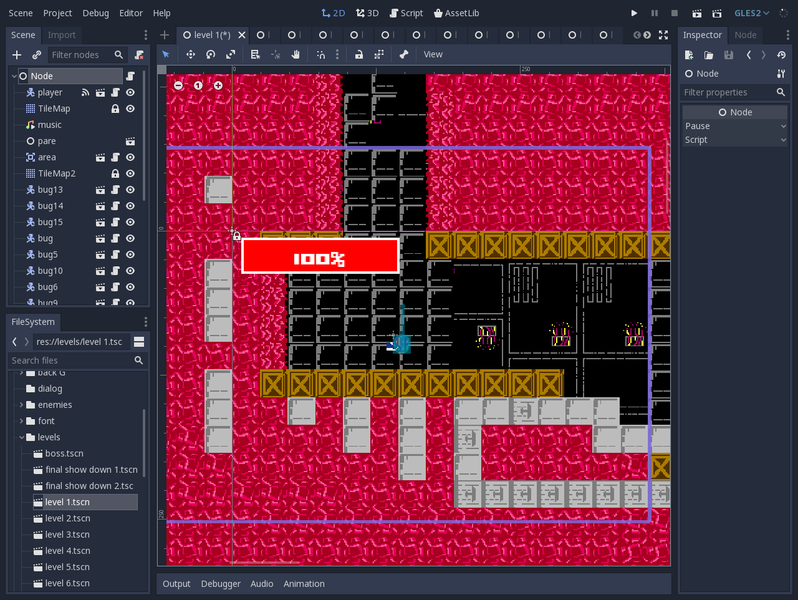
\includegraphics[width=13cm]{archivos/imagenes/Godot-captura.png}
	\caption[Interfaz de Godot.]{Interfaz de Godot\footnotemark.}
	\label{Godot interfaz}
\end{figure}
\footnotetext{Imagen extraída de Wikipedia \url{https://es.wikipedia.org/wiki/Godot}}

\subsection{\glsentrylong{ia}}
Además de los \gls{tfg} he decidido\footnote{Guiado por los conocimientos de mi tutor, que tiene los conocimientos y experiencia en el tema necesarios para aconsejarme los documentos en los que he de fijarme} realizar la lectura del libro \textit{Learning from Data: A Short Course} de \citefullauthor{LearningFromData}, un experto en el mundo de la Inteligencia Artificial. Un libro en el que da la iniciación, de forma teórica, al mundo del \gls{ml}, explicando el algoritmo más básico que es el perceptrón, con las fórmulas matemáticas y las propiedades estadísticas necesarias para entenderlo. Y las clases de la asignatura de Razonamiento Automático impartidas por mi tutor Francisco J. Gallego-Durán.

El \gls{ml} en videojuegos se puede usar para entrenar a un oponente del jugador, en cuyo caso es interesante definir varios niveles de dificultad. Puesto que entrenar a una máquina para que sea mejor que un humano en un juego es una tarea relativamente sencilla, la verdadera dificultad reside en que la máquina aprenda a jugar varios niveles, con los que se pueda ajustar al nivel de habilidad del jugador, de manera que siempre suponga un reto para el jugador batir a la máquina, pero que no sea tan extremadamente difícil que el jugador pierda las ganas de continuar jugando porque ha perdido el interés.
\\
Una segunda manera de usar el \gls{ml} es entrenando un agente para que bata los récords en un juego ya existente, es decir, que sustituya la posición del humano en el juego, de manera que consiga imitar o mejorar el comportamiento de un humano en el juego. Siendo el objetivo a batir un enemigo del juego, completar un mapa, o enfrentarse contra un humano. Esta segunda, es la manera que más se ha popularizado últimamente porque es algo más vistoso, y los ejemplos más conocidos son:
\begin{description}
	\item[MuZero:] Está desarrollada por DeepMind, empresa filial de  Google. Es capaz de ganar a cualquier humano jugando al Ajedrez, al Shogi y al Go.
	\item[AlphaStar:] También desarrollada por DeepMind. Es capaz de ganar a cualquier humano jugando al Star Craft, un juego de PC que trata de reunir recursos estratégicamente para combatir a tus enemigos.
	\begin{figure}[H]
		\centering
		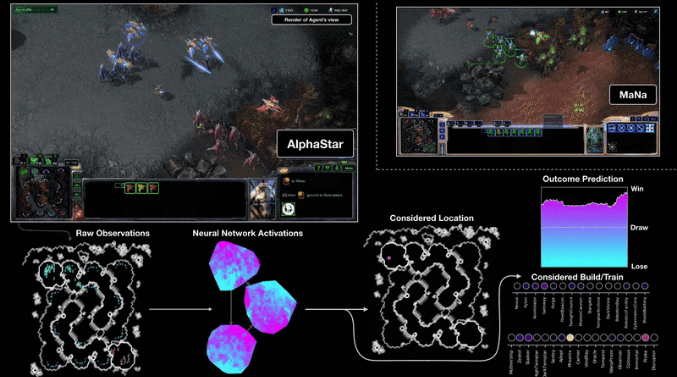
\includegraphics[width=15cm]{archivos/imagenes/alphastar-playing.png}
		\caption[Alphastar jugando al Star Craft.]{Alphastar jugando al Star Craft\footnotemark.}
	\end{figure}
	\footnotetext{En la web robologs.net \url{https://robologs.net/2019/02/03/alphastar-la-ia-de-google-aprende-a-jugar-a-starcraft-ii/}}
	\item[Dino T-Rex:] Este no es una \gls{ia}, sino más bien un juego que se activa en Chrome cuando no tienes acceso a Internet. He decidido añadirlo en esta lista ya que al ser un juego tan conocido y sencillo, existen muchas personas que han decidido empezar programando su primera \gls{ia} con este, por ello, podemos encontrar muchos ejemplos simples de como entrenar a un agente en Internet.
	\begin{figure}[H]
		\centering
		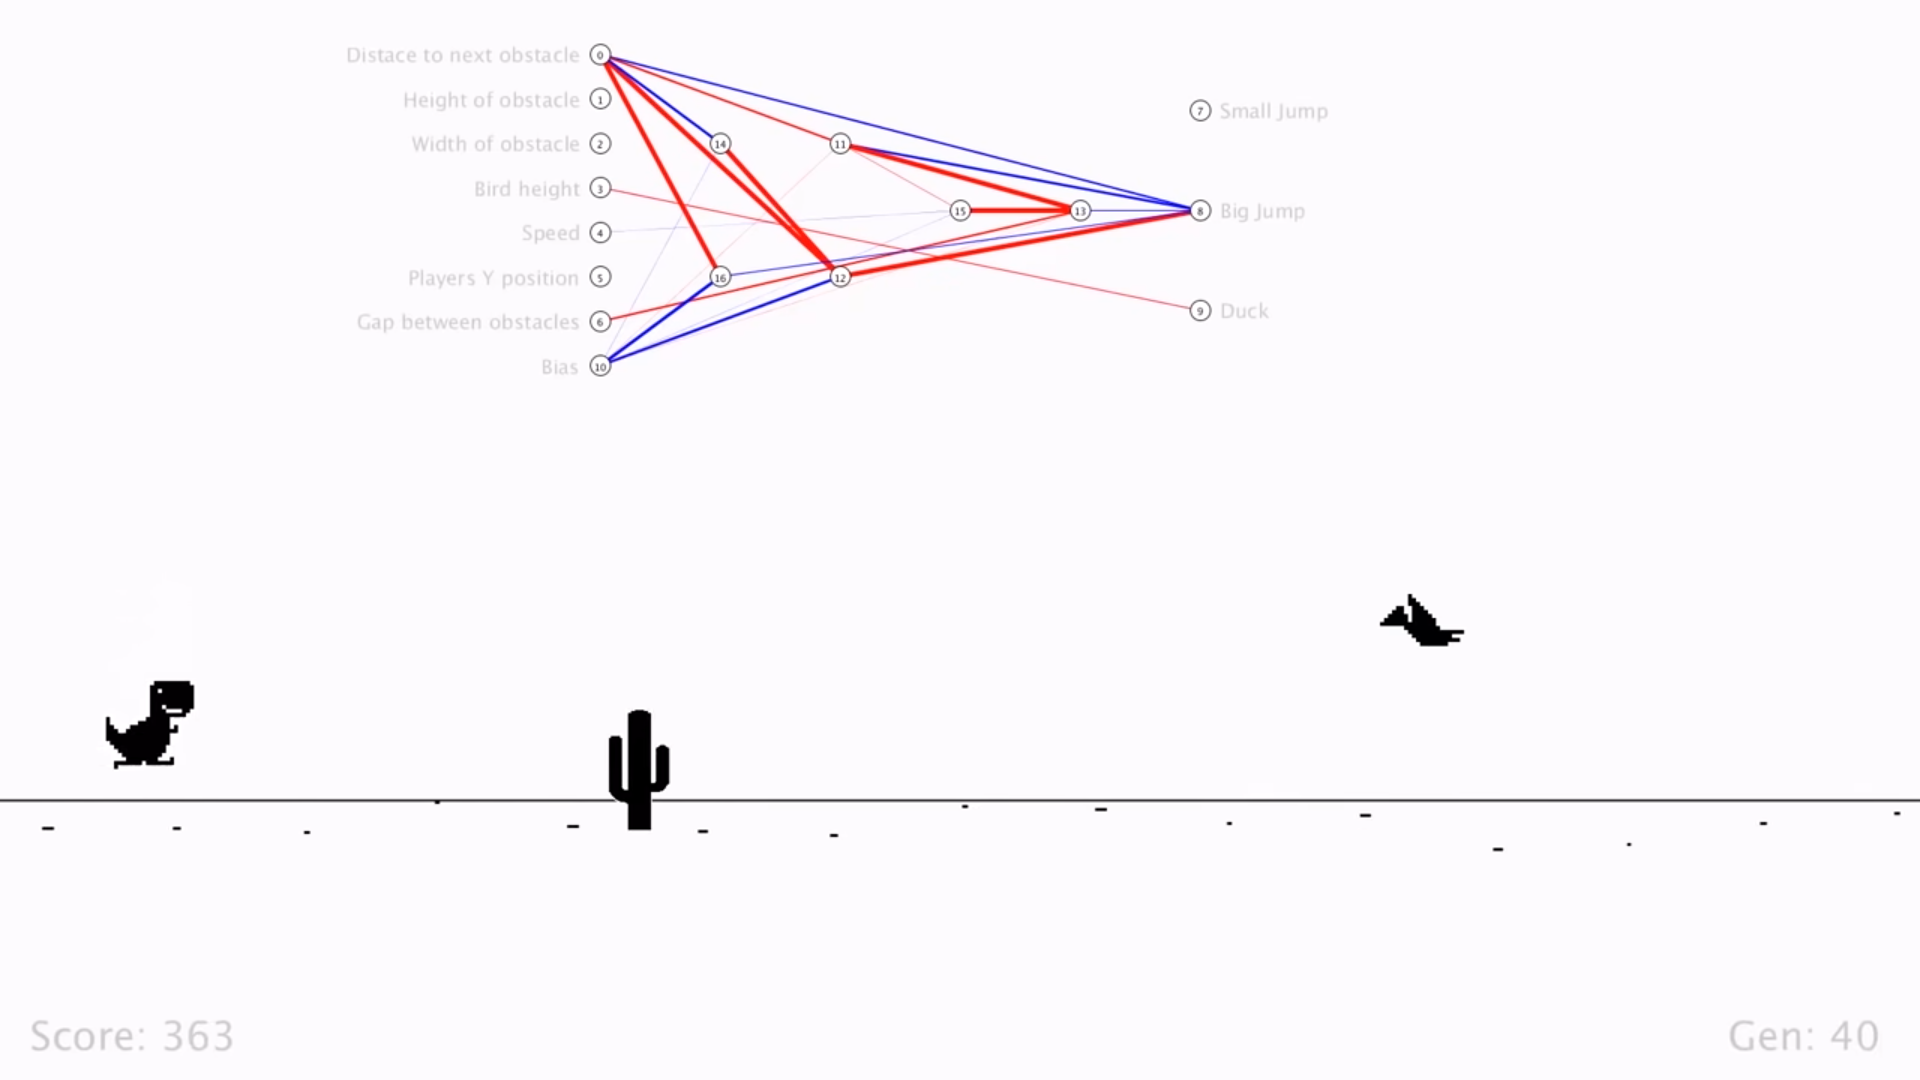
\includegraphics[width=15cm]{archivos/imagenes/dino-trex-ia.png}
		\caption[\gls{ia} aprendiendo a jugar a Dino T-Rex.]{\gls{ia} aprendiendo a jugar a Dino T-Rex\footnotemark.}
	\end{figure}
	\footnotetext{Del canal de YouTube de Evan Even \url{https://www.youtube.com/watch?v=sB_IGstiWlc}}
	\item[Emergent Tool Use from Multi-Agent Interaction:] No se trata de ningún juego para humanos, pero es una herramienta desarrollada por OpenAI, una organización sin ánimo de lucro centrada en el desarrollo de \gls{ia} de código abierto. Trata de unos agentes que tienen que aprender a jugar al escondite, jugando dos contra dos, teniendo que aprender tanto los que pillan como los que son pillados a ganar. Estos agentes llegaron a desarrollar finalmente técnicas que explotan los fallos de las físicas del juego.\footnote{Para más información sobre el tema en el siguiente enlace se encuentra el paper \url{https://openai.com/blog/emergent-tool-use/}}
\end{description}
\todo{He descubierto que si pongo "H" en las figuras, en lugar de "h", se colocan exactamente donde quiero, pero en algunos casos pasa esto de que el texto se separa mucho. ¿Está bien así?¿O lo dejo como antes?}	% Plantilla: Se muestran listas
%%%%%%%%%%%%%%%%%%%%%%%%%%%%%%%%%%%%%%%%%%%%%%%%%%%%%%%%%%%%%%%%%%%%%%%%
% Plantilla TFG/TFM
% Escuela Politécnica Superior de la Universidad de Alicante
% Realizado por: Jose Manuel Requena Plens
% Contacto: info@jmrplens.com / Telegram:@jmrplens
%%%%%%%%%%%%%%%%%%%%%%%%%%%%%%%%%%%%%%%%%%%%%%%%%%%%%%%%%%%%%%%%%%%%%%%%

\chapter{Objetivos}
\label{objetivos}
El primer objetivo del proyecto es crear un motor, lo suficientemente genérico como para que pueda ser usado por otros videojuegos. Este motor estará separado de las mecánicas del juego como son el comportamiento de las físicas, las colisiones, o el renderizado, ya que todas estas funcionalidades son diferentes en cada juego, dependerá de si queremos hacer un renderizado 3D, 2D, si queremos un comportamiento distinto de las colisiones, etc. Por lo que crearé un motor para el videojuego, con los conocimientos que habré adquirido mediante la formación previa. 

Luego, el principal objetivo de este proyecto es desarrollar un juego en el que la persona que se decida a jugarlo aprenda los conocimientos básicos sobre \gls{ml}. La tarea del jugador será entrenar a la \gls{ia} de manera que sirva como un oponente capaz de ganar a otros jugadores, y también a otras \gls{ia}.
\\
El usuario podrá tanto entrenar al agente en una arena de juego, como poner al agente a entrenar con los datos extraídos de alguna partida, o los datos extraídos de la arena, \todo{e incluso ajustar los parámetros de la \gls{ia} manualmente para experimentar con ellos??}. También, el jugador podrá enfrentarse contra el agente, y en última instancia, el objetivo final es enfrentar la \gls{ia} de un jugador contra la de otro jugador que ofrezca su \gls{ia} como rival. 
\\
El concepto de la idea es bastante sencillo, crearé el conocido juego Pong, un juego con mecánicas básicas y fácil de entender, y añadiré dificultades al mismo, que puede ser trivial para un humano superarlas, pero algo más difícil para una máquina. La motivación para añadir estas dificultades al juego es que el juego del Pong tiene tan pocos elementos (una pala rival, una pala que eres tú mismo, y la pelota) que hace muy sencillo que una \gls{ia} pueda aprender a jugar contra un humano a un nivel decente. Es tanto así, que en una parte del  desarrollo habré creado solo el Pong, y podré a entrenar a dos perceptrones, y veremos en los resultados si con sólo dos perceptrones es posible que una \gls{ia} aprenda a jugar al Pong.
\\
Posteriormente, cuando haya añadido dificultades al juego, programaré tecnologías más avanzadas que el perceptrón, como puede ser una red neuronal. Y entonces haré pruebas con estas nuevas dificultades añadidas, para ver si realmente el agente consigue aprender a jugar a este remix del juego del Pong.
\\
Y por último, añadiré una interfaz amigable, para que el producto final pueda ser manejado por un usuario sin necesidad de editar el código o ficheros de configuración, sino que pueda hacerlo todo desde la interfaz. Tanto entrenar, como seleccionar los conjuntos de datos para la \gls{ia}, como ajustar parámetros, como elegir la opción de jugar, todo desde la interfaz.

Por último, he de remarcar algo más abstracto de los objetivos del proyecto en sí, no del juego: la mayor parte del software usado será de desarrollo propio, es decir, intentaré minimizar el uso de librerías de terceros (sólo usándolas para tareas menos relevantes en el proyecto). Así que el motor del videojuego, el videojuego y la \gls{ia} en sí serán desarrollados desde cero en el lenguaje C/C++. Esto es así porque el objetivo final no es obtener una productividad absoluta, utilizando tecnologías existentes que me permitirían terminar el proyecto en una cantidad de tiempo mucho menor, sino que tengo que estudiar estas tecnologías desde la raíz, analizarlas, y entender en profundidad cómo funcionan estos tres campos en los que se centra mi \gls{tfg}.

Más concretamente, los objetivos son:
\begin{itemize}
	\item Estudiar tecnologías de motor de videojuegos e implementarlas en el proyecto.
	\item Conocer cuáles son las librerías y tecnologías mínimas para desarrollar el videojuego.
	\item Analizar la evolución del uso de la \gls{ia} en el mundo de los videojuegos.
	\item Analizar el estado del arte actual del \gls{ml} en videojuegos.
	\item Diseñar e implementar prototipos simples de mecánicas de juego.
	\item Diseñar e implementar técnicas de \gls{ml} para que les sea fácilmente utilizable a los jugadores.
	\item Diseñar métricas para poder medir si la \gls{ia} ha cumplido con los objetivos.
	\item Crear una interfaz para que estas métricas sean visibles ajustables por los jugadores reales.
	\item Diseñar diferentes modos de juego en los que el jugador real pueda entrenar a su \gls{ia}.
	\item Crear un modo de juego en el que dos jugadores aporten su \gls{ia} y se visualice el enfrentamiento.
\end{itemize}		% Plantilla: Se muestran tablas
%%%%%%%%%%%%%%%%%%%%%%%%%%%%%%%%%%%%%%%%%%%%%%%%%%%%%%%%%%%%%%%%%%%%%%%%
% Plantilla TFG/TFM
% Escuela Politécnica Superior de la Universidad de Alicante
% Realizado por: Jose Manuel Requena Plens
% Contacto: info@jmrplens.com / Telegram:@jmrplens
%%%%%%%%%%%%%%%%%%%%%%%%%%%%%%%%%%%%%%%%%%%%%%%%%%%%%%%%%%%%%%%%%%%%%%%%

\chapter{Metodología}
\label{metodologia}
La metodología de este proyecto se basa en algunas metodologías ágiles estudiadas en las asignaturas de la carrera dedicadas a ello, es una metodología iterativa. Esto nos permite a mi tutor y a mí, ver en qué partes necesito más ayuda y en cuáles podemos avanzar más rápido, pudiendo así adaptar perfectamente la velocidad del desarrollo en cada iteración.
\begin{figure}[h]
	\centering
	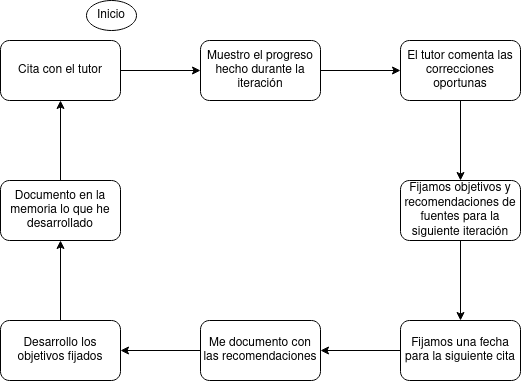
\includegraphics[width=15cm]{archivos/imagenes/diagrama-de-metodologia.png}
	\caption{Metodología de trabajo seguida durante el desarrollo.}
	\label{diagrama de metodologia}
\end{figure}

El ciclo comienza en el cuadrado superior izquierdo, y salvo la primera iteración, en la que no hubo que mostrar el progreso, y por lo tanto no hubo nada que corregir, el resto de iteraciones siguieron el patrón que se puede ver en la figura \ref{diagrama de metodologia}.

Todas las iteraciones duran entre 3 y 4 semanas. Para cada iteración se concierta una cita entre el tutor y el alumno, se pone un objetivo de trabajo y una fecha para la próxima quedada. En esta reunión se exponen los trabajos concretados en la anterior, que han de estar finalizados y se propondrán los siguientes.
\\
Cada iteración o sprint consta de una parte de formación, en la que el alumno, orientado por el tutor, adquiere conocimientos sobre lo que se va a trabajar\footnote{Esto puede tratarse tanto de vídeos formativos como de libros u otras lecturas recomendadas.}, y lo pone en práctica en el proyecto. Finalmente, todo lo hecho durante ese sprint se documenta en el documento del \gls{tfg} y se muestra el progreso al tutor, quién valora el trabajo y propone alguna corrección en caso de ser necesaria.

\section{Control de versiones}
Para gestionar el control de versiones usaré la famosa herramienta Git\footnote{Software creado por Linus Torvalds para el control de versiones.} debido a lo extendido que está, tanto en el mundo laboral, como para uso personal, y lo fácil que es de usar a través de plataformas como GitHub\footnote{Plataforma de Microsoft, utilizada comúnmente para compartir código de forma abierta en Internet, que implementa el control de versiones de Git.}. Esto me permite compartir el código fácilmente con mi tutor, tener un respaldo en la nube de mi trabajo, y además volver a una versión anterior del código estable, en el caso de que cambie cosas que no debería haber hecho.
\\
El momento en el que tomo una instantánea del código, o como se le conoce hacer ``commit'', es al acabar una idea previamente planteada. Por ejemplo, si quiero implementar el funcionamiento de la gravedad: pienso cómo se haría, lo implemento y compruebo que funciona, y el proyecto ya está listo para hacer ``commit''. Si posteriormente se encuentra algún defecto se modificará el código y se hará otro ``commit'' con un mensaje descriptivo, comentando cuál era el defecto arreglado, y esto ayudará a evitar errores como borrar o modificar partes del código que no debía. 

\section{Herramientas de trabajo}
\label{herramientas}
A parte de las anteriormente mencionadas \textbf{Git} y \textbf{GitHub}, voy a utilizar las siguientes herramientas:
\begin{itemize}
    \item \textbf{Visual Studio Code:} Se trata de un editor de texto creado por Microsoft, derivado de su \gls{ide}\footnote{Entorno de desarrollo integrado en español, herramienta que te ayuda en tareas de programación como auto-completar código, compilar, etc.} Visual Studio, pero open source, multiplataforma y simplificado. Dispone de un montón de extensiones que lo hacen compatible con cualquier lenguaje que disponga de una.
    \item \textbf{TeXstudio:} Este \gls{tfg} está siendo escrito en \LaTeX por lo que es necesario un editor para facilitar el uso del lenguaje, con correcciones y para poder pre-visualizar el documento final.
    \item \textbf{xelatex:} Es el compilador que utiliza TeXstudio para compilar los documentos \LaTeX.
    \item \textbf{Gimp:} Herramienta de creación y edición de imágenes, útil para poder crear o modificar las imágenes necesarias para ilustrar algunas partes del \gls{tfg}.
    \item \textbf{draw.io:} Aplicación online para la creación de diagramas, que también usaré para ilustrar el \gls{tfg}.
    \item \textbf{Google Meet:} Aplicación online para mantener reuniones, usada para reunirme con mi tutor.
    \item \textbf{g++:} Compilador de C++ desarrollado por GNU para compilar en sistemas basados en Unix.
    \item \textbf{clang++:} Otro compilador de C++ alternativo, ya que, aunque siguen el estándar de C++, uno te puede dar los errores que otro no, o mostrarlos de una forma distinta, y eso puede ayudar entenderlos o evitar errores en el futuro.
    \item \textbf{gdb:} Un depurador de C++, útil para encontrar errores en el código. Es compatible con Visual Studio Code, por eso, y su gran facilidad de uso es el elegido. 
    \item \textbf{make:} Herramienta de gestión de dependencias, para compilar y recompilar de forma automática el código y generar el ejecutable.
    \item \textbf{Arch Linux:} Sistema operativo basado en Linux, que utilizo en mi portátil para el desarrollo del \gls{tfg}.
\end{itemize}	% Plantilla: Se muestran figuras
%%%%%%%%%%%%%%%%%%%%%%%%%%%%%%%%%%%%%%%%%%%%%%%%%%%%%%%%%%%%%%%%%%%%%%%%
% Plantilla TFG/TFM
% Escuela Politécnica Superior de la Universidad de Alicante
% Realizado por: Jose Manuel Requena Plens
% Contacto: info@jmrplens.com / Telegram:@jmrplens
%%%%%%%%%%%%%%%%%%%%%%%%%%%%%%%%%%%%%%%%%%%%%%%%%%%%%%%%%%%%%%%%%%%%%%%%

\chapter{Desarrollo}
\label{desarrollo}

Como he comentado en el apartado de metodología, el desarrollo del \gls{tfg} se divide en iteraciones, de las cuales ha habido un total de 9, y en los siguientes apartados expondré cuál es el trabajo que se ha desarrollado en el transcurso de las mismas.
Por lo tanto, este apartado será el más extendido del \gls{tfg}, ya que en él explico detalladamente cuál es el trabajo que he ido haciendo, ordenado en el tiempo, y dividido en los tempos que me he reunido con mi tutor.

\section{Primera iteración: desarrollo del motor}
El \textbf{7 de julio de 2020} nos citamos por la herramienta Google Meet, y hablamos sobre cuál era mi objetivo con este \gls{tfg}, lo definimos y presentamos la propuesta. Además, como no tenía conocimientos sobre motores de videojuegos, me sugirió empezar viendo su curso para desarrollar un motor en C/C++. No concertamos una segunda cita ya que empezaba la época de verano, y quedamos en que cuando comenzara el curso y hubiera desarrollado mi motor volvería a ponerme en contacto con él.

\subsection{Script de construcción del proyecto}
Lo primero que hice fue, antes de ponerme a programar el motor, crear el archivo Makefile, este es el fichero que la herramienta Make ya mencionada en el apartado \ref{herramientas} de herramientas, utiliza como Build Script. De esta forma no tendría que compilar todos los archivos uno a uno. Y además, separando las librerías del resto del código, así no tendrían que ser re-compiladas cada vez que necesite crear un ejecutable, ya que este es un proceso que tarda unos segundos pero se repite muchas veces, por lo que estos segundos ahorrados a lo largo del desarrollo podrían llegar a ser muchos minutos, incluso horas, de espera ahorrados.

Como no voy a explicar todo el archivo línea por línea, lo haré con las partes más importantes del mismo. 
\begin{itemize}
	\item La macro \textbf{COMPILE}, recibe cinco parámetros. Es usada para compilar todos los objetos antes de ser enlazados. Recibe los siguientes parámetros:
	\begin{enumerate}
		\item Compilador a usar (gcc, g++, clang++, etc.)
		\item Nombre del objeto que se genera
		\item Archivos de código fuente
		\item Dependencias
		\item Flags para el compilador
	\end{enumerate}
	\begin{lstlisting}[style=C, caption={Macro Compile del Makefile},label=macro-compile]
		define COMPILE
		$(2) : $(3) $(4)
			$(1) -c -o $(2) $(3) $(5)
		endef
	\end{lstlisting}
	\item La instrucción \textbf{\$(APP)} o \textbf{game}, que es el nombre del ejecutable final. 
	\begin{itemize} 
		\item Depende de todos los objetos. 
		\item Enlaza todos los objetos y librerías, y genera el ejecutable
	\end{itemize}
	\begin{lstlisting}[style=C, caption={Enlazado de los objetos y las librerías para generar el ejecutable.},label=library-linking]
	$(APP) : $(OBJSUBDIRS) $(ALLOBJ)
		$(CC) -o $(APP) $(ALLOBJ) $(LIB) $(CCFLAGS)
	\end{lstlisting}
	\item La instrucción \textbf{clean}, que elimina los objetos para re-compilarlos desde cero.
	\item La instrucción \textbf{libs} y \textbf{libs-clean}, que compila y elimina pero con las librerías.
\end{itemize}
Dentro de la carpeta lib tenemos otro Makefile que sirve para compilar las librerias, las cuales tienen su propio Makefile también, muy parecido al ya mencionado.

\subsection{Motor de videojuego}
Comenzamos el desarrollo del videojuego creando el motor, pues sin él, no se puede avanzar con los otros puntos. Se trata de un motor \gls{ecs}\footnote{Conocido en español como Sistema de Entidades y Componentes. Es un patrón de desarrollo para motores de videojuegos.} el cual se basa en que las entidades son manejadas por el motor, mientras que los componentes (como físicas, renderizado, colisiones, etc.) son añadidos desde el juego. Pero el motor es el que se encarga de añadir los componentes a las entidades o destruirlos. Y los sistemas son los encargados de actualizar el estado de los componentes.

Para que el motor se comporte de manera eficiente con la caché, todos los componentes de un mismo tipo se almacenan seguidos en memoria, para que así, cada sistema del juego pida un solo tipo de componente de todas las entidades del juego. Ya que se ha demostrado que leer un dato de la caché es, de media, 200 veces más rápido que leerlo de la RAM, y cuando el programa pide un dato, no solo se carga ese dato pedido, sino un stream de datos. Además, cabe mencionar que la caché lee de la memoria RAM por líneas, nunca lee menos del tamaño de una linea, como se puede apreciar en el ejemplo de la figura \ref{Memoria RAM y CPU}, con una linea de caché de 64 bytes de tamaño.
\begin{figure}[H]
	\centering
	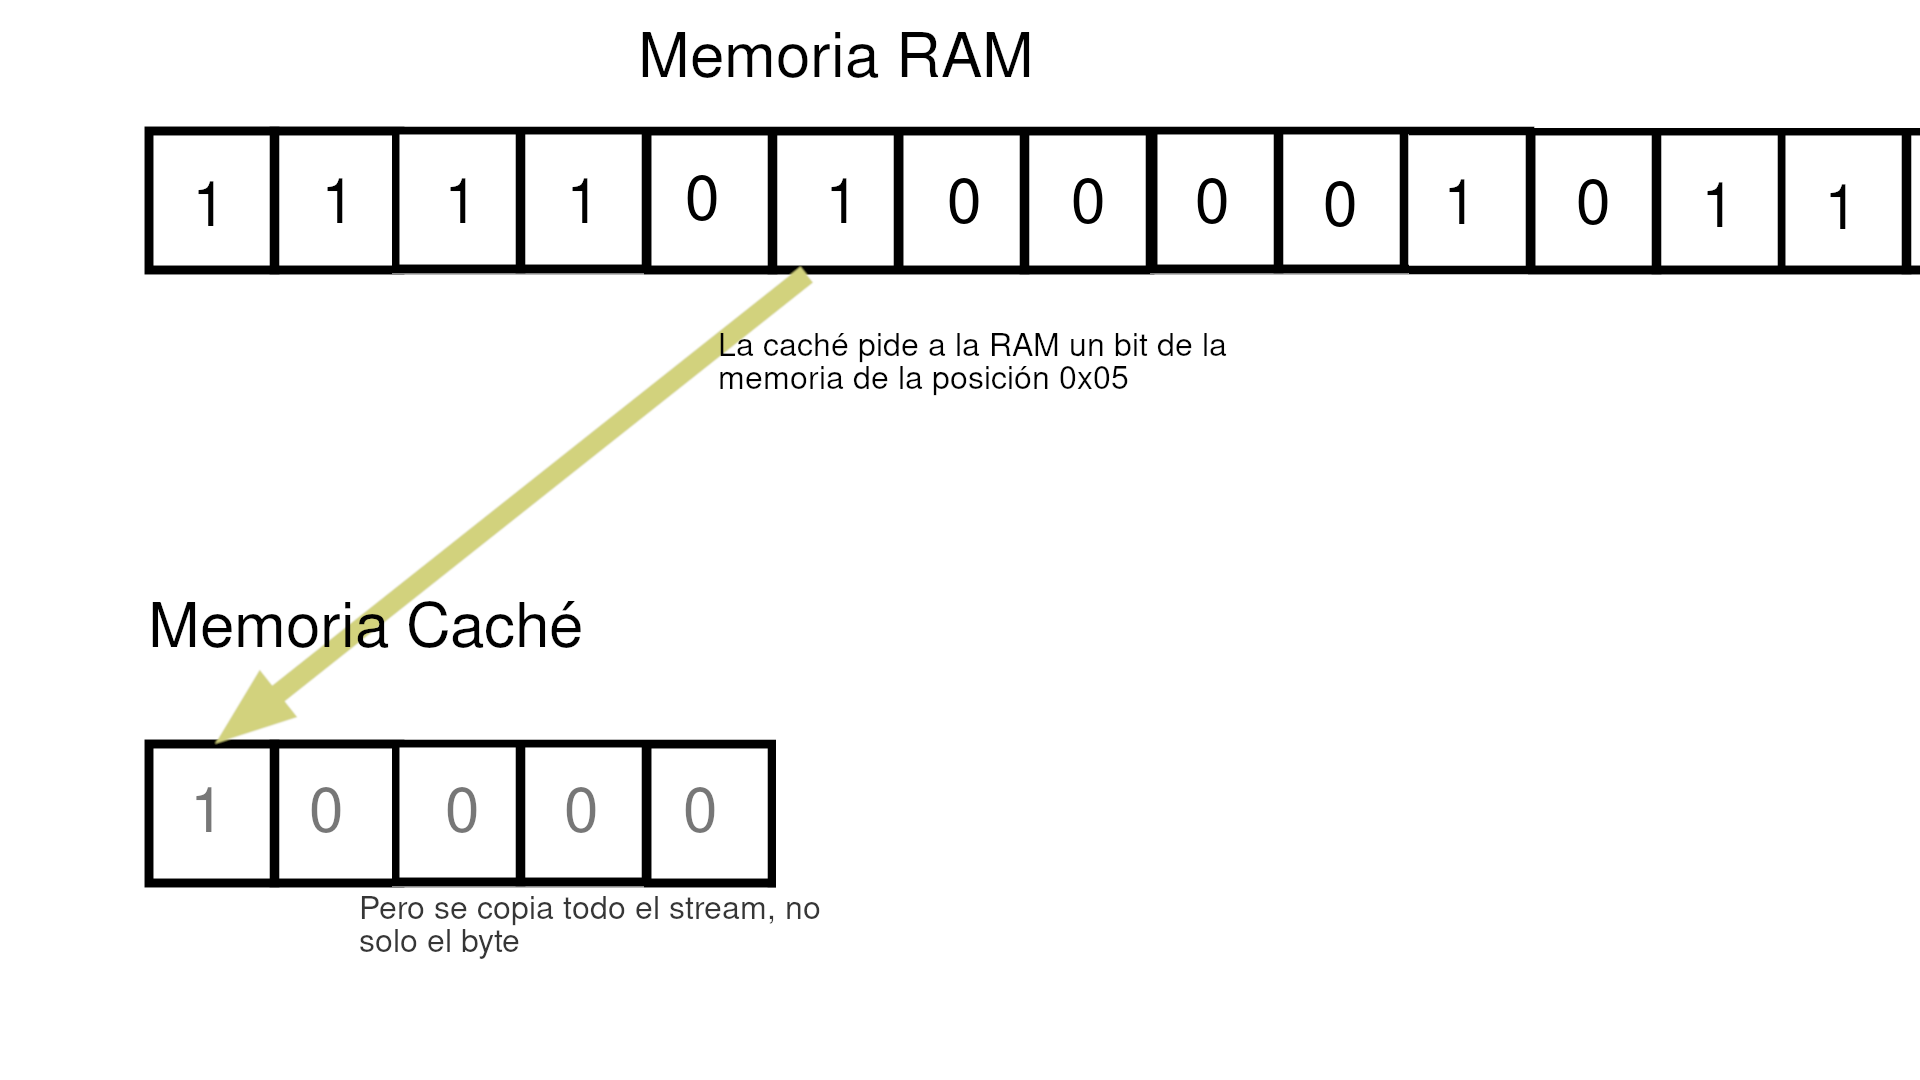
\includegraphics[width=15cm]{archivos/imagenes/comportamiento-memoria-cpu-ram.png}
	\caption{Comportamiento de la memoria CPU cuando lee de la RAM.}
	\label{Memoria RAM y CPU}
\end{figure}

¿Cómo se pueden alinear los datos en memoria según su tipo? La implementación ha sido usando la librería unordered\_map de C++, con la cual podremos usar un mapa, es decir, una estructura de datos en la que uno es el identificador (el tipo de dato, en este caso), y otro es el valor almacenado (un vector de componentes, en este caso).  Esto trae un problema consigo, porque el ``tipo de dato'' no es un tipo básico en C++, esto explicaré más adelante cómo lo solucionaremos. 

Cada sistema es encargado de un tipo de componente, para así poder recorrer la memoria de forma lineal como ya hemos mencionado antes (el sistema de físicas recorre todos los componentes de físicas existentes en el motor), y así optimizar el uso de la caché. Aunque como veremos adelante, eso no es del todo sencillo, porque en ocasiones, actualizar el estado de un componente depende del estado de un segundo\footnote{Un ejemplo de esto es al actualizar los componentes de colisiones, es inevitable tener que solicitar el componente de física.}.
\\
Todas las clases del motor están dentro del espacio de nombres \textbf{ECS}.

\begin{figure}[H]
	\centering
	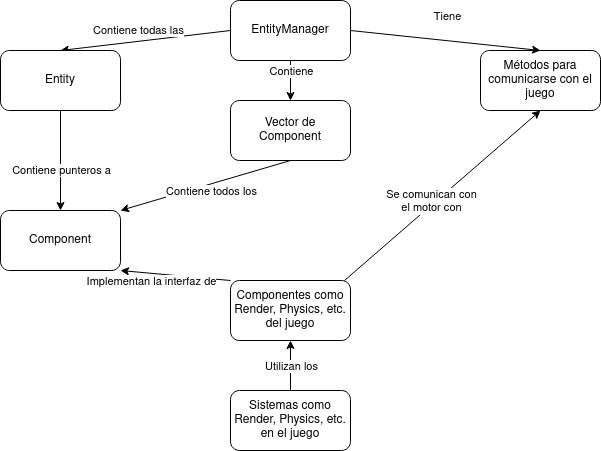
\includegraphics[width=15cm]{archivos/imagenes/Diagrama-funcionamiento-motor.png}
	\caption{Para qué se utiliza EntityManager. Diagrama de construcción propia.}
	\label{diagrama entitymanager}
\end{figure}

Como vemos en la figura \ref{diagrama entitymanager}, la clase EntityManager\_t es la clase que usará el juego para comunicarse con el motor. Tiene los métodos necesarios para almacenar, solicitar y borrar tanto entidades como un componente de una entidad. Estos componentes son almacenados en m\_components, así que EntityManager\_t tiene un fuerte acoplamiento con ComponentStorage\_t, y si quisiéramos otra implementación del motor donde los componentes no sean parte de las entidades, haría falta aplicar cambios sobre este acoplamiento.

La clase Entity\_t tiene un vector de punteros hacia sus componentes, la ventaja de esto es que no hace falta que el componente tenga un ID, y por lo tanto, la búsqueda del componente es más rápida. El inconveniente es que hay que tener mucho cuidado con dónde está almacenado el componente, ya que el encargado de darle una zona en la memoria es ComponentStorage\_t, y si este modifica la posición del componente, el puntero en Entity\_t no apuntará a la zona correcta de la memoria. 

Por último, el motor también proporciona una interfaz para la comunicación entre la entrada de teclas en el juego y el sistema operativo. Esto lo hace utilizando algunas funciones de la librería TinyPTC, que se activan cuando una tecla es pulsada.\footnote{Para un desarrollo más amplio de cómo funcionan estas funciones, ver el curso de \cite{CursoMotorC++}.}

\subsection{Dificultades a destacar}
Algunas de las dificultades de crear un motor genérico, que pueda aceptar cualquier tipo de componente es que hay que hacer las funciones template, de no ser así, cada vez que queramos añadir un nuevo componente habría que añadir una nueva función, la cual sería una copia de otra y eso podría generar errores futuros al tener que cambiar lo mismo en todas las copias. Y no solo eso, el mayor problema sería que el motor no estaría desacoplado del juego, y no sería útil para cualquier juego, sino habría que modificarlo en función del juego que queramos crear.

Un segundo problema es que la clase Entity\_t almacena punteros a Component\_t, pero como ComponentBase\_t hereda de Component\_t es posible que trabaje con los componentes del juego. ¿Por qué añadir este nivel de indirección? El problema lo hemos mencionado antes: el tipo de un componente no es un tipo básico de C++. Por lo tanto, no podremos usar una estructura de mapa para almacenar los componentes del juego según el tipo de forma lineal en memoria.
\\
Lo solucionamos de la siguiente manera: la clase Entity\_t almacena un unordered\_map de ``tipo de componente'' a ``puntero a Component\_t''. Component\_t tiene un método estático getComponentTypeID() que devuelve un entero que será el identificador único del componente durante la ejecución del programa. De esta manera, el juego podrá añadir tantos tipos de componente distintos como quiera, sin tener que preocuparse por el identificador, que es tarea del motor.
\begin{lstlisting}[style=C-color, caption={Cómo tener un número variable de componentes, sin tener que añadir un nuevo identificador con cada componente nuevo.},label=static-method]
	static ComponentTypeID_t getComponentTypeID() noexcept {
		static ComponentTypeID_t typeID { ++nextTypeID };
		return typeID;
	}
\end{lstlisting}
Pero, ¿qué significa el anterior código? Para entenderlo, hemos de saber para qué sirve la palabra reservada ``static'': cualquier variable que sea estática existirá al principio del programa, y continuará hasta el final de la ejecución del mismo. Por lo tanto, el método getComponentTypeID() devolverá siempre el mismo identificador, ya que typeID se define una sola vez en la ejecución del programa, y no cada vez que se llama al método, y nextTypeID es un miembro estático de la clase padre Component\_t que inicialmente es cero.
\\
Pero esto ocasiona el problema de que todos los componentes devolverán el mismo identificador. ¿Cómo hacemos que cada componente tenga el suyo propio? C++ tiene templates, lo que significa que, en tiempo de compilación, un código template se replicará por cada tipo diferente que haya sido instanciado la clase template. Por lo tanto, cada componente del juego, deberá heredar de ComponentBase\_t, de esta manera se crearán tantos ComponentBase\_t con su método estático getComponentTypeID() como componentes distintos tenga el juego.

Otro problema relacionado con la creación de un motor genérico es que, en algunos casos, las funciones del juego se usarán en un ámbito constante, y otras no, por lo que las funciones que queramos que sirvan para ambos casos, han de estar replicadas de forma que devuelvan un valor constante o no. El problema del código repetido que se solventa haciendo uso del las conversiones con static\_cast<>(), podemos ver un ejemplo a continuación:
\begin{lstlisting}[style=C-color, caption={Ejemplo de conversion de un método constante a no constante},label=no-constant-conversion]
	template<typename CMP_t>
	const CMP_t* getComponent() const {
		auto type = CMP_t::getComponentTypeID();
		auto it = m_components.find(type);
		if(it != m_components.end()) 
		return static_cast<CMP_t*>(it->second);
		return nullptr;
	}
	
	template<typename CMP_t>
	CMP_t* getComponent() {
		const CMP_t* cmp = const_cast<const Entity_t*>(this)->getComponent<CMP_t>();
		return const_cast<CMP_t*>(cmp);
	}
\end{lstlisting}
Hay que recordar siempre, que las conversiones han de ser de un método constante a uno no constante. De no ser así, podría suceder que el método no constante modifique algo, y devolvamos algo que ha mutado en el método constante.

\section{Segunda iteración: desarrollo del Pong}
El \textbf{29 de octubre de 2020} tuvimos la segunda iteración donde le conté a mi tutor lo que había aprendido y desarrollado, y acordamos los siguientes objetivos:
\begin{itemize}
  \item Aprender a usar \LaTeX.
  \item Comenzar la estructura de la memoria.
  \item Ver el curso de Yaser Abu-Mostafa sobre \gls{ml}.
  \item Crear un pong donde las palas se controlen aplicando aceleración y no velocidad.
  \item Almacenar los datos de la partida en \gls{csv}.
  \item Programar un perceptrón.
\end{itemize}

\subsection{Creación del juego}
Al igual que, para continuar con el desarrollo del TFG, lo primero era crear un motor funcional, antes de poder implementar los conocimientos de \gls{ia} hay que crear un juego. Como mencioné en la introducción (apartado \ref{introduccion}), esta es la parte más creativa, y puede que sea la parte que más tiempo me lleve pero no necesita prácticamente mucha formación. Por lo que, lo primero que voy a hacer es programar el clásico juego del Pong para que, posteriormente, la pala rival sea controlada por un perceptrón. 
\\
El juego tiene una estética simple, hecha sin sprites, solo coloreando en la ventana un color uniforme para cada entidad:
\begin{figure}[H]
	\centering
	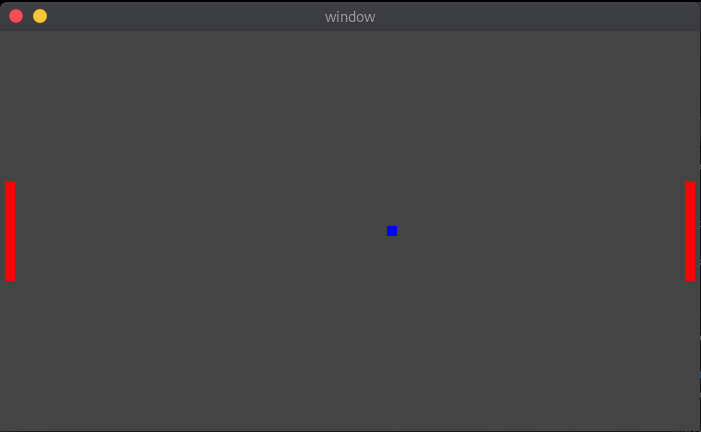
\includegraphics[width=15cm]{archivos/imagenes/pong.png}
	\caption{Imagen del primer juego, Pong.}
\end{figure}

Además, al juego le he añadido un menú, en el que eliges si quieres jugar contra un humano, para recoger los movimientos de la pala, si quieres entrenar la \gls{ia}, con algún \gls{csv} de datos de alguna partida anteriormente jugada, y una tercera opción de jugar contra una \gls{ia}. Y por supuesto la opción de salir.
\begin{figure}[H]
	\centering
	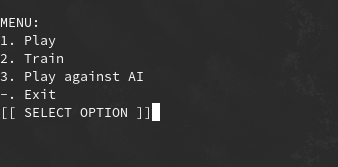
\includegraphics[width=15cm]{archivos/imagenes/menu-del-pong.png}
	\caption{Primer menú del juego.}
\end{figure}

Programar el juego no fue algo especialmente complicado, dado que durante el curso de motor de videojuegos en C++ de \citefullauthor{CursoMotorC++}, se implementan sistemas y componentes como los de colisiones, físicas, etcétera, muchos solo había que adaptarlos al Pong y ya funcionaban. Además tuve que añadir algunos extra como un sistema de puntuación, por ejemplo. Y no tuve que hacer nada de arte gráfico por el momento, ya que con unos rectángulos que se pueden generar con un for, era suficiente para entender el juego, como se puede ver en la imagen del juego.

\subsection{Resolución del resto de trabajo}
Almacenar los datos en un \gls{csv} no fue una tarea extremadamente difícil. Cada sistema tiene un método dump() y un array donde se almacenan los datos de cada frame, y cada 100 frames se guarda en un \gls{csv} los datos de ese sistema durante la partida.

La estructura de la memoria la estoy haciendo en base la plantilla que nos proporciona José Manuel Requena en GitHub \footnote{\url{https://github.com/jmrplens/TFG-TFM\_EPS}}, y fijándome en la estructura del libro de Yaser y los \gls{tfg} de mis compañeros anteriormente mencionados, de esta manera puedo tener un conocimiento de cómo escribir un documento oficial, comparando algunos anteriormente hechos.

Y por último, he comenzado a intentar implementar, sin éxito, los conocimientos sobre el perceptrón. La pala rival no responde en función de los parámetros del juego después de haber sido entrenada, por lo que estoy entendiendo mal los conceptos de \gls{ml} explicados en \citep{LearningFromData}. En la próxima cita con mi tutor le expondré este problema para ver cómo podremos darle solución.

\section{Tercera iteración: problemas con el aprendizaje}
El \textbf{26 de noviembre de 2020} volvimos a quedar para ver mi trabajo durante el último mes, y nos encontramos con varios problemas. Los problemas serían los objetivos para la próxima iteración, y fueron los siguientes.

\begin{enumerate}
	\item A pesar de tener formación en inglés y de haber cursado alguna asignatura en la carrera sobre \gls{ia}, me resultaba difícil comprender los conceptos que Yaser explicaba en el curso, así que mi tutor, me recomendó la lectura del libro en el que se basan estas charlas, en el cual se extiende más y hace más fácil la comprensión del mismo.
	\item A pesar de tener el juego del Pong ya funcionando, el día de antes estuve añadiendo código, cosa que hizo que dejara de funcionar. El código estaba bajo el control de versiones de Git, sin embargo, no sabía utilizar la herramienta por completo así que no supe volver a una versión anterior.
	\item No sabía cómo comenzar a escribir mi \gls{tfg} ni qué escribir en cada una de sus secciones.
\end{enumerate}

Después de estos problemas, ralentizamos el ritmo de desarrollo y acordamos que para la siguiente iteración: habría aprendido a usar Git por completo, habría revisado algunos de los \gls{tfg} de mis compañeros, con un posterior desarrollo del mío propio, y habría leído \textit{Learning from data: a short course} \cite{LearningFromData}

Durante esta iteración no hubo un gran avance del proyecto, debido a que todas las tareas que propusimos fue que arreglara los errores que había tenido hasta el momento, y el tiempo entre esta y la siguiente era más reducido de lo normal.

\section{Cuarta iteración: juego con el perceptrón}
El \textbf{17 de diciembre de 2020} tuvimos la última cita del año, revisamos los objetivos marcados en la anterior iteración y ya había desarrollado brevemente cada campo de la memoria del \gls{tfg}, implementado el perceptrón y aprendido a usar Git. Sin embargo, no habiendo terminado de leer \textit{Learning from data: a short course}, y con las ideas un poco confusas, el perceptrón no respondía correctamente, por lo que los objetivos para la siguiente iteración serían:
\begin{itemize}
  \item Completar toda la memoria con las cosas hechas hasta el momento.
  \item Ver las clases de Razonamiento Automático de mi tutor.
  \item Arreglar la implementación del perceptrón.
  \item Hacer funcionar el perceptrón dentro del juego.
  \item Rehacer el sistema de recogida de datos en \gls{csv}.
\end{itemize}

\subsection{Desarrollo total del perceptrón}
El problema principal con el perceptrón fue que, debido a algunas similitudes entre entrenar y jugar, implementé el código de tal forma que todo estaba en la misma clase. Mi tutor me explicó que la parte del entrenamiento está separada del juego y me dijo que viese las clases de Razonamiento Automático, de esta manera conseguiría aclarar las ideas tan dispersas que tenía.

Lo que hace el perceptrón es recibir los datos relevantes de la partida, como son las físicas de la pelota y del jugador controlado por la \gls{ia}. Entonces, los datos son una X de la fórmula \ref{suma ponderada}, los pesos del perceptrón ya entrenado son representados con una W, y el número total de datos es N.
\begin{equation}
	\sum_{i=0}^NX_{i}*W_{i}
	\label{suma ponderada}
\end{equation}
El resultado de ese sumatorio será positivo o negativo, y no es necesario añadir en la fórmula el límite, sino que el límite es 0 ya que entre los datos se ha añadido el threshold como una entrada con valor 1, y entre los pesos se ha añadido uno extra al principio para que se ajuste al igual que el resto de pesos. En el caso de dar positivo, significará que la suma ha superado el threshold (representado como $w_o(t)$ en la figura \ref{perceptron}), lo que significa que la \gls{ia} manda al juego pulsar esa tecla de la pala, y en caso de ser negativo no. A cada tecla (arriba y abajo) le corresponde un perceptrón, que es el que decide si esta es pulsada o no.

Para entrenar al perceptrón, paso previo para jugar contra él porque sino, no existirá un fichero con la configuración del mismo, lo que hago es:
\begin{enumerate}
	\item Generar un array de pesos aleatorios y calcular el error que generan estos pesos.
	\item Se repite N veces el siguiente proceso:
	\begin{enumerate}
		\item Se calcula el error de los pesos que se quiere ajustar.
		\item Si este perceptrón con estos pesos es mejor que el mejor hasta el momento (tiene un error menor), se guarda.
		\item Del perceptrón ajustado, se elige uno al azar entre todos los puntos que no ha acertado si pulsar o no pulsar. 
		\item Si la tecla no fue pulsada, y debía serlo, se suma al peso el valor del input del perceptrón. Si la tecla fue pulsada, y no debía serlo, se resta. (Es decir, teniendo M entradas, la operación de suma o resta se hace desde 0 hasta M, al peso i se le suma/resta el input i).
	\end{enumerate}
	\item El perceptrón que haya dado menor error se guarda en un fichero para poder ser usado en el juego.
\end{enumerate}

El perceptrón ya funcionaba correctamente después de ver las primeras clases de Razonamiento Automático, ya que conseguí entender las dudas que me quedaban sobre el tema. Dando un resultado totalmente jugable, ya que no era invencible, ni tampoco tan malo como para no convertirse en un reto. El error que no permitía funcionar de forma correcta era una mala proporción de los datos entregados al agente durante el entrenamiento. El \gls{csv} de datos tenía una cantidad mucho mayor de ejemplos de ``no pulsar'', y muy pocos de ``sí pulsar'', por lo que en la mayoría de casos, el perceptrón entrenado se quedaba parado. Esto tenía varias posibles soluciones, entre ellas ajustar el cálculo del error (es decir, que un fallo de no pulsar cuando sí hay que hacerlo subiese más el valor error), y por la que opté yo, que era ajustar los datos de tal manera que quedasen distribuidos la mitad del ejemplo de frames pulsando y la otra mitad no pulsando. Esto trajo otro pequeño inconveniente, y era que los datos extraídos de ``no pulsar'' eran del principio de la partida, y esos frames de ejemplo no eran lo suficientemente representativos, por lo que opté por coger los frames aleatorios.

\subsection{Desarrollo de una red neuronal}
Además, en las clases de Razonamiento Automático, Francisco J. Gallego-Durán explica cómo funciona una red neuronal y cómo programarla, incluso, invita a los alumnos a crearla de tal forma que sea diferente a la ya creada por él, sin el uso de la librería vector de C++ para conseguir una mayor eficiencia en lo que se refiere a los tiempos de ejecución. Por lo que después de aprender los conceptos con sus clases, me dispuse a programar mi propia red neuronal para después introducirla en el juego cuando este se convirtiera en algo más complejo que una pala rebotando una bola, sin embargo, no era consciente de las facilidades que aporta la clase vector, y me topé con varios problemas durante el desarrollo.
\\
Algunos de estos problemas fueron, tener que sobrescribir el constructor de copia por no comportarse cómo deseaba, tener que manejar el puntero de los datos según si se quería contar el threshold o no (recordemos que uno de los motivos por los que haría una implementación propia de la clase vector sería para obtener más eficiencia a la hora de leer los datos), etc.
\\
El hecho de tener que detenerme a estudiar cómo funcionan algunas de las facilidades que aporta vector, y escribir las partes de la memoria que faltaban me llevó todo el tiempo que quedaba hasta esta quinta iteración. Ya había solventado los problemas de la anterior y había alcanzado los objetivos propuestos, por lo que llegué con todo el trabajo hecho a esta.

\subsection{Recogida de datos de la partida}
Además, un segundo problema de concepto fue el cómo recoger los datos. En primera instancia cada sistema se encargaba de recoger sus datos en el \gls{csv}, de tal manera que como los sistemas necesarios para que la \gls{ia} aprenda son las físicas y el sistema de input, había dos archivos que correspondían a la misma partida, con distinto nombre y distintos datos, pero tremendamente acoplados, por lo que mi tutor sugirió que los recoja de manera externa a sus sistemas, todos los datos necesarios en un mismo \gls{csv}, así que ese era otro objetivo para la siguiente iteración. 

Y por último, me dijo que no era necesario almacenar datos en array e intentar optimizar la escritura de estos datos en un fichero, ya que el juego no es tan complejo como para que se ralentice por abrir y escribir un archivo en cada frame. Conseguí solucionarlo rápidamente. Al principio de la partida creo unas referencias a los objetos que necesito guardar, y en cada frame abro el archivo y lo escribo con los datos actuales. No es la forma más eficiente de hacerlo, pero para un juego tan sencillo funciona perfectamente.

\section{Quinta iteración: mejorando el juego}
El \textbf{14 de enero de 2020} tuvimos la siguiente iteración, los objetivos marcados para la siguiente iteración han sido más ambiciosos de lo normal, así que no es necesario que estén completos, pero mi tutor comentó que sería bueno al menos intentarlo, de tal manera que fueron:
\begin{enumerate}
	\item Arreglar algunos defectos de la memoria debidos a mi falta de experiencia escribiendo documentos oficiales.
	\item Desarrollar el Pong Plus, un juego inspirado en el Pong, pero con ciertos añadidos que lo hacen más complejo
	\begin{itemize}
		\item Minions en el centro del campo (pequeñas palas que ayudan a su compañero a ganar).
		\item Los minions son capaces de rebotar la pelota, y su movimiento es solo en el eje y.
		\item Los minion pueden morir a causa de un disparo, de ser así reaparecerán tras unos segundos.
	\end{itemize}
	\item Añadir un sistema de recogida de datos que tenga en cuenta los nuevos datos de la partida, y que también funcione para los minions.
	\item El jugador debe poder elegir si jugar con la pala o con el minion, para así obtener el correspondiente \gls{csv} que servirá de entrenamiento.
	\item Añadir una opción para poder configurar el entrenamiento recibido desde el juego.
	\item Portar el juego para Windows, dado que actualmente solo está compilado para Linux.
\end{enumerate}

\subsection{Pong Plus}
Lo primero que hice esta vez fue: cambiar los colores del juego, añadir un marcador dentro de la pantalla y una linea en medio, para intentar mejorar la estética del juego. El resultado está en la figura \ref{primera vista del pong plus}.

\begin{figure}[H]
	\centering
	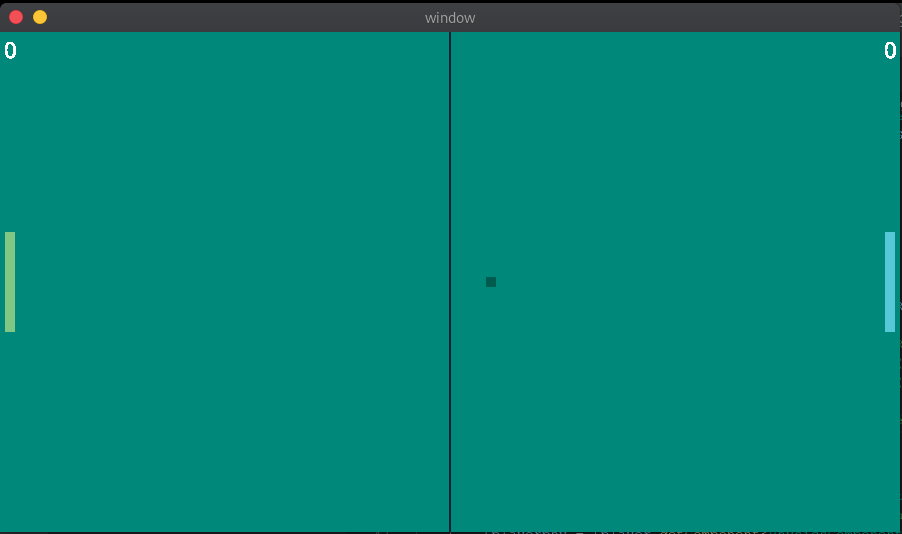
\includegraphics[width=12cm]{archivos/imagenes/pong-nuevos-colores.png}
	\caption{Imagen del Pong con nuevos colores y marcador.}
	\label{primera vista del pong plus}
\end{figure}

Lo que hice en segunda instancia, no estaba dentro de los objetivos que nos habíamos marcado pero decidí hacer un menú, pensando que sería algo sencillo, pero me llevó más tiempo del que imaginaba. Para hacer el menú necesitaba renderizar texto, y para no alargar más el desarrollo, decidí añadir una librería que se usa para renderizar texto en formato true type llamada stb\_truetype\footnote{La librería es del tipo conocido como only-header, se encuentra en github junto con otras utilidades \url{https://github.com/nothings/stb}}. De esta manera, también podría usar los números del marcador como texto. Para moverte por el menú se usarán las flechas del teclado de arriba y abajo. El resultado lo puedes ver en la figura \ref{primer menu del juego}.

\begin{figure}[H]
	\centering
	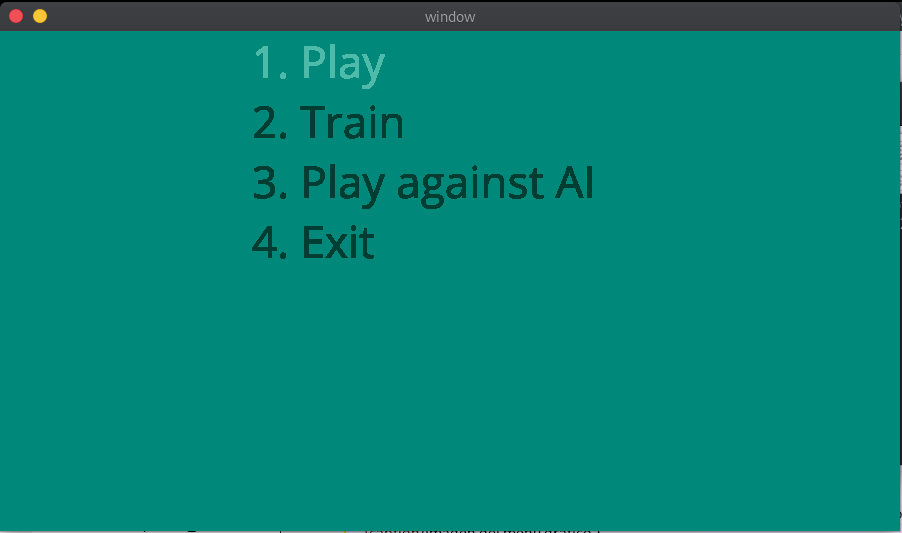
\includegraphics[width=12cm]{archivos/imagenes/menu-grafico-integrado-en-el-juego.png}
	\caption{Imagen del menú gráfico.}
	\label{primer menu del juego}
\end{figure}

Una vez acabado el menú, que además te permite seleccionar qué \gls{csv} quieres usar entre todos los que has generado jugando, añadí los minions y unas paredes, las cuales habría que romper para poder pasar tu bola al campo enemigo. Esto es posible porque las bolas traspasan las paredes que son de su mismo color.

\begin{figure}[H]
	\centering
	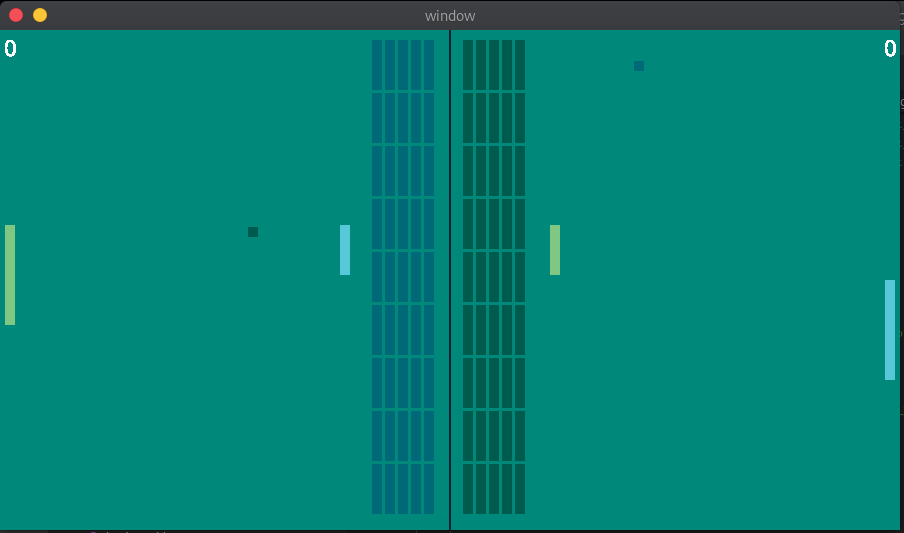
\includegraphics[width=12cm]{archivos/imagenes/pong-plus-con-minions-y-paredes.png}
	\caption{Imagen de la primera versión del Pong Plus.}
\end{figure}

\subsection{Compilación para Windows}
Lo último que hice en este periodo fue compilar el juego para Windows. Mi tutor explica en el curso de videojuegos \cite{CursoMotorC++} cómo modificar el fichero de construcción (Makefile) para compilar para Windows desde una máquina con Linux (comúnmente conocido como cross-compiling), y en la librería de TinyPTC descargable, también hay unos ficheros de código específicos para Windows, por lo que la única tarea que me quedaba por hacer era modificar las partes del código donde se incluye la versión de TinyPTC de Linux e incluir la versión de Windows, y recompilar el proyecto. 
\\
Pero cuando probé el juego en Windows, se ejecutaba correctamente, pero no respondía ante la entrada por teclado. Y es que la codificación del teclado en Windows no es la misma que la de X11, por lo que creé un fichero en el que definí los valores de la variable dependiendo de si la compilación está activada para Windows o para Linux. Posteriormente usé ``\#ifdef''\todo{Aquí tampoco sé si usar cursiva, comillas... o qué usar} que hace que el compilador use esa parte del código sólo se compile si la macro está presente en la linea de compilación, o si está definida previamente en otro fichero incluido por este, de esta manera lo podía combinar con ``\#else'' para definir las teclas del juego para Windows cuando construya el juego para Windows, y las teclas de Linux cuando compile para este sistema operativo.

\section{Sexta iteración: aprendizaje mediante backpropagation}
\label{sexta iteracion}
El \textbf{11 de febrero de 2021} tuvimos una nueva reunión, en la cual los objetivos marcados fueron:
\begin{enumerate}
	\item Continuar mejorando defectos de la memoria y desarrollando los nuevos hitos de las nuevas iteraciones.
	\item Implementar Dear ImGui en el proyecto
	\begin{itemize}
		\item Estudiar cómo se usa.
		\item Sustituir TinyPTC por OpenGL3 para poder renderizar tanto el juego como las ventanas.
		\item Diseñar menús para manejar el juego.
	\end{itemize}
	\item Programar el algoritmo de backpropagation.
	\item Poder elegir tanto los ficheros de datos de entrenamientos como los ficheros de pesos para el juego.
	\item Añadir un campo de entrenamiento para que no sea necesario que haya dos jugadores para recoger datos de entrenamiento.
	\item Añadir un algoritmo básico para cuando no exista un fichero de pesos pero que se pueda jugar contra una \gls{ia}.
\end{enumerate}

Comencé la iteración con ilusión, viendo documentación de Dear ImGui y estudiando cómo implementar la librería en mi proyecto. Pero antes de empezar a implementarlo debía acabar lo que empecé en la anterior iteración, la red neuronal. Es cierto que en la anterior iteración la red neuronal ya era capaz de resolver el problema de la XOR con un entrenamiento aleatorio, es decir, probar una asignación de pesos aleatoria para la red, y si obtenía mejores resultados que la mejor red hasta el momento, se sustituían los pesos de la red neuronal por estos nuevos.
\begin{figure}[H]
	\centering
	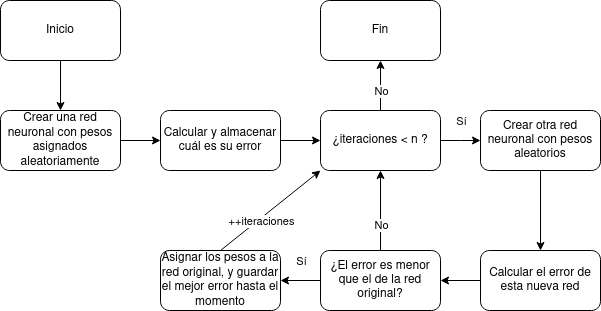
\includegraphics[width=15cm]{archivos/imagenes/Algoritmo-red-neuronal-aleatorio.png}
	\caption{Algoritmo de aprendizaje aleatorio. Esquema de construcción propia.}
	\label{Algoritmo aleatorio}
\end{figure}
Es un algoritmo que podría funcionar en algunos casos, pero requiere de un número mucho más alto de iteraciones de media, así que no es lo suficientemente eficiente. Por lo que me dispuse a desarrollar el algoritmo de backpropagation.

\subsection{Desarrollo de Backpropagation}
Durante esta iteración apliqué Backpropagation a la red neuronal ya creada antes, como puedes ver en el apartado \ref{marco teorico backpropagation}, y me di cuenta de un grave error que cometí desarrollando la red neuronal, como se puede apreciar en el apartado \ref{aleatorio vs backpropagation resultados}, comparo la velocidad a la que aprende la red neuronal usando los dos diferentes tipos de entrenamiento, y originalmente las conclusiones que saqué fueron las siguientes:
\\
El algoritmo aleatorio consigue aprender más rápido que el de backpropagation porque el problema de la puerta XOR es demasiado sencillo, y por lo tanto la estructura de la red es demasiado simple. Llegando a concluir que el algoritmo aleatorio encuentra la solución el 80\% de las veces después de iterar 1000 veces, mientras que el algoritmo de backpropagation encuentra la solución sólo el 1.4\% de las veces, y para llegar al 80\% habría que iterar 100000 veces. Cuando le comenté estas conclusiones a mi tutor me dijo que era muy extraño que una red neuronal tardara tanto en aprender el problema de la XOR, siendo tan simple la estructura de la red (dos neuronas de entrada, una capa oculta con cuatro neuronas, y una de salida). Para hallar estos datos ejecuté cada uno de los anteriores experimentos 10000 veces y así conseguir que la media fuese algo significativo, y que la varianza afectase lo mínimo posible.

¿Dónde se encontraba el problema? No parece una conclusión lógica. El problema, como recuerdo en la cita del principio de esta memoria, estaba entre la silla y el teclado. Y es que había programado mal el constructor de la clase de la red neuronal, este asignaba mal los punteros de una capa de la red a su siguiente capa. De tal forma que para calcular el delta de backpropagation sólo se calculaba bien en la última capa, que no depende de ninguna capa posterior, por lo tanto sólo variaban los pesos de las neuronas de la última capa, y por eso era tan costoso que la red aprendiese, porque el resto de capas se quedaban con el valor inicial aleatorio y no variaban en todo el entrenamiento. En la figura \ref{problema aprendizaje red neuronal} puedes ver un ejemplo ilustrativo del problema.
\begin{figure}[H]
	\centering
	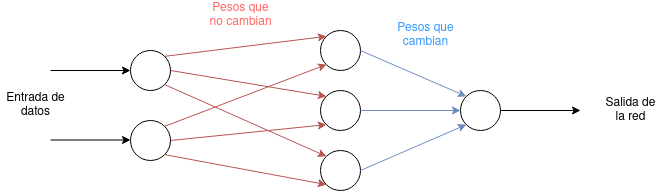
\includegraphics[width=15cm]{archivos/imagenes/problema-de-aprendizaje-red.png}
	\caption{Problema de aprendizaje de la red neuronal.}
	 \label{problema aprendizaje red neuronal}
\end{figure}

\subsection{Graves problemas durante el desarrollo}
\todo{Añadirlo en un anexo.}
Como ya he mencionado en el apartado de herramientas de trabajo, yo he desarrollado este proyecto con Linux, pero por motivos relacionados con la carrera, es necesario que también tenga instalado Windows en el ordenador. Después de una actualización, este último dejó de funcionar, y cuando opté por solucionar el error, se cargó la partición de Linux. Por suerte, todo el trabajo de este \gls{tfg} estaba bajo el control de Git, y en la nube de GitHub, por lo que los daños en ese sentido eran mínimos. Pero tenía que recuperar el resto de cosas.

No voy a contar cómo fue la recuperación del sistema operativo ya que no procede en esta memoria, pero esto juntado con los trabajos de las asignaturas de la universidad, me hizo perder más de una semana, por lo que esta iteración quedó prácticamente en nada.

\section{Séptima iteración: creación de menús}
El día \textbf{11 de marzo de 2021} volvimos a tener una llamada de revisión de trabajo y nuevas propuestas, pero según se desarrolló la anterior iteración, mi tutor y yo acordamos que para esta acabaría lo ya acordado, prestando especial atención en el desarrollo de la memoria, ya que era lo que más trabajo requería en la situación en la que estaba, y conociendo que ya quedaba poco tiempo para la entrega del \gls{tfg}.

\subsection{Dear ImGui}
Por lo tanto, comencé a implementar Dear ImGui en el proyecto. El primer paso era sustituir TinyPTC por OpenGL3, así que eso hice: fui al sistema de Render, que se encarga de abrir la ventana y dibujar sobre ella, y cambié todo el código necesario en este punto. Ahora la ventana la abriría con OpenGL3 y cada frame dibujado por software mediante el sistema de render se pasaría a OpenGL3 también, de esta manera Dear ImGui solo tendrá que dibujar las ventanas encima de mi interfaz.
\\
El siguiente paso fue aprender a dibujar una ventana dentro del juego, y así fue, algo bastante sencillo porque aparece en el código de ejemplo que ellos tienen en el proyecto.

\begin{figure}[H]
	\centering
	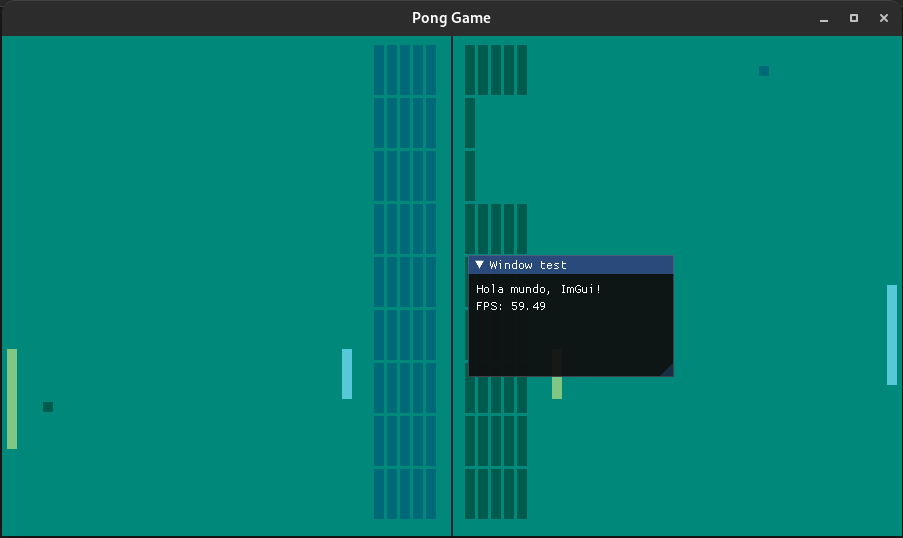
\includegraphics[width=15cm]{archivos/imagenes/ventana-dentro-del-juego.png}
	\caption{Ventana dentro del juego.}
\end{figure}
Pero como los menús de los juego no suelen ser en una ventana, decidí hacerlo en pantalla completa. No es el mejor diseño, pero ya servía para poder manejarse  dentro del juego.
\begin{figure}[H]
	\centering
	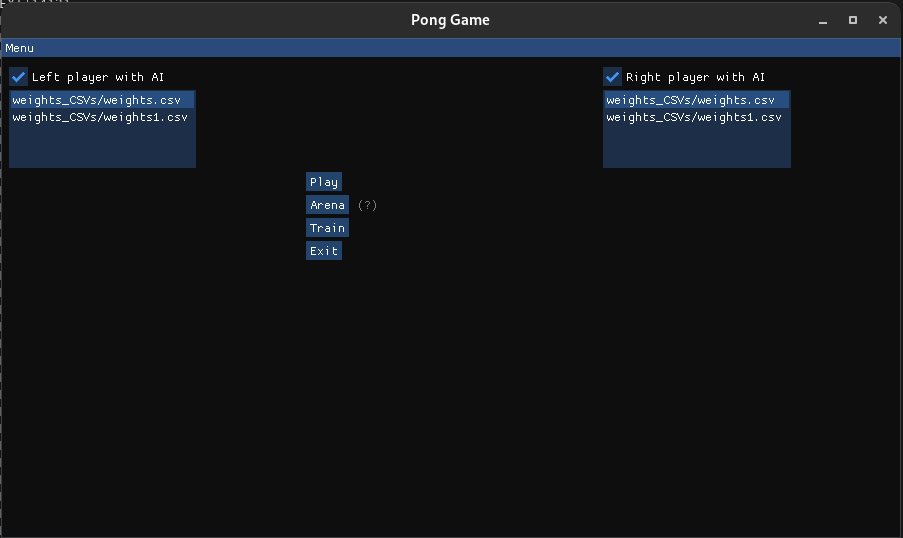
\includegraphics[width=15cm]{archivos/imagenes/menu-del-juego.png}
	\caption{Menú del juego.}
	\label{Menu del juego}
\end{figure}
Ahora ya, teniendo las herramientas que nos da Dear ImGui, me dispuse a desarrollar un menú en el cuál el jugador, pueda decidir cómo entrenar a su \gls{ia}, y además que pueda ver de manera gráfica cómo va aprendiendo y cuáles son las consecuencias de cambiar los parámetros de entrenamiento de la \gls{ia}. Puedes ver el menú de entrenamiento en la figura \ref{Menu de entrenamiento}.

\subsection{Campo de entrenamiento}
El campo de entrenamiento es el apartado de arena que puedes ver en la figura \ref{Menu del juego}, que te pondrá a jugar en el mismo campo de siempre, pero sin rival, cuando la pelota llega a la pared del rival rebotará, de esta manera el jugador podrá reaccionar a diferentes situaciones de partida (con el minion rival en una posición, las bolas en otras posiciones, con velocidades distintas, etc.) que servirán como dataset para un posterior entrenamiento en el menú de entrenamiento.
\begin{figure}[H]
	\centering
	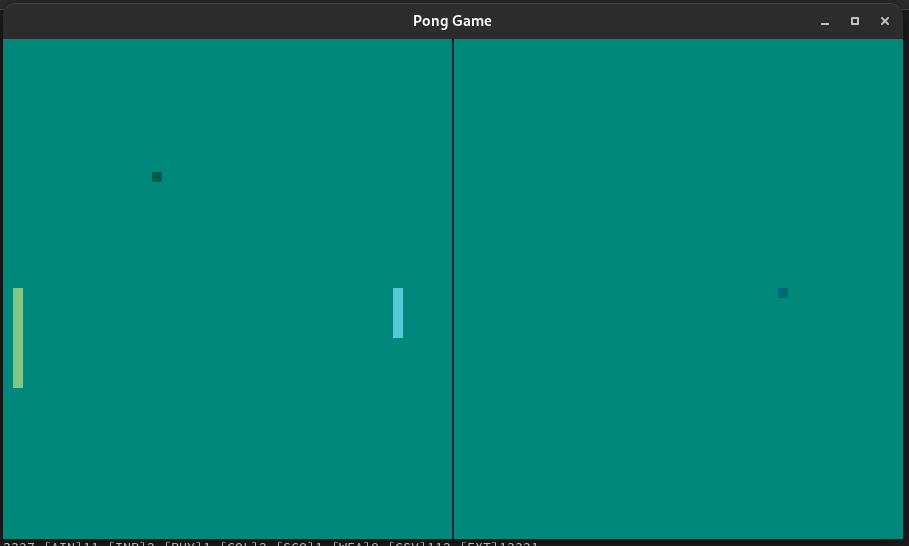
\includegraphics[width=15cm]{archivos/imagenes/arena-de-entrenamiento.png}
	\caption{Arena de entrenamiento.}
\end{figure}

Después de obtener todos los datos podremos ir al siguiente menú de la figura \ref{Menu de entrenamiento}, donde el jugador elegirá los parámetros que considere oportunos para entrenar la \gls{ia}. Entre ellos podrá cambiar, la cantidad de muestras que usa de cada tipo (de esta manera soluciono el problema ya conocido desde la neurona, y es que hay una gran cantidad de ejemplos de no tocar en la muestra), el ratio de aprendizaje que aplicará, la estructura de la red neuronal, y por supuesto, el número de iteraciones que hará Backpopagation. Por último, abajo del todo se puede apreciar una gráfica en la cuál pone a su derecha "\% of error". En esta gráfica el usuario verá el progreso de cómo va disminuyendo el error a lo largo del tiempo.
\begin{figure}[H]
	\centering
	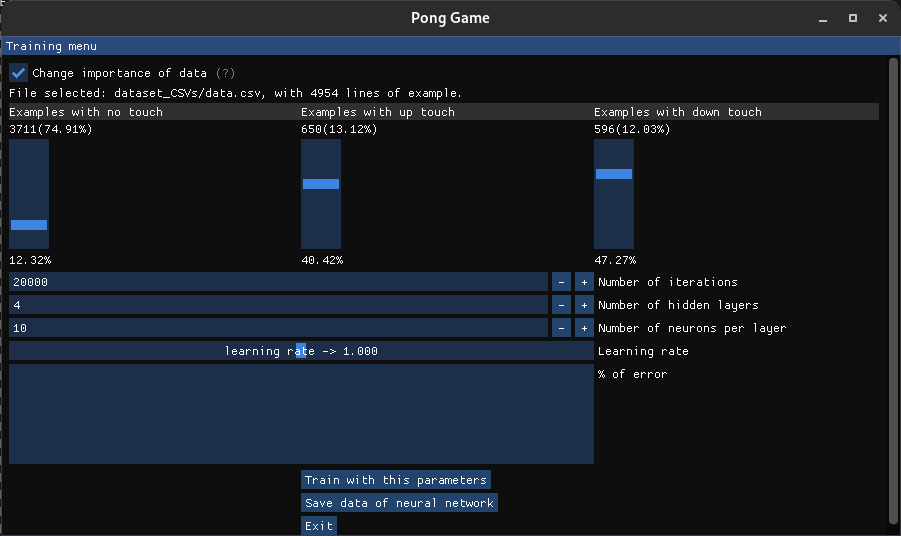
\includegraphics[width=15cm]{archivos/imagenes/menu-de-entrenamiento.png}
	\caption{Menú de entrenamiento del juego.}
	\label{Menu de entrenamiento}
\end{figure}

\section{Octava iteración: perfilando el proyecto}
\label{octava iteracion}
El \textbf{13 de abril de 2021} ya solo quedaba un mes para la confirmación de la entrega del proyecto en el C3, por lo que ya tendríamos que tener todo acabado para la siguiente fecha, o a punto de acabar para confirmar la entrega. Los objetivos para esta iteración, por lo tanto, fueron los siguientes:
\begin{enumerate}
	\item Añadir capturas a la memoria, puesto que eran escasas y eran necesarias para entenderla.
	\item Añadir apartado de resultados a la memoria, con tablas, imágenes, y demás representaciones.
	\item Arreglar el método de entrenamiento de la \gls{ia}.
	\item Añadir un algoritmo básico para cuando no exista un fichero de pesos pero que se pueda jugar contra una \gls{ia}.
\end{enumerate}

\subsection{Arreglo del entrenamiento}
Cuando desarrollé el algoritmo de aprendizaje de la red neuronal inicialmente, decidí añadir un factor de importancia a cada acción (pulsar arriba, abajo, o no pulsar). Esto fue porque ya tuve problemas inicialmente con el perceptrón y sé que la cantidad de ejemplos de cada tipo está desproporcionada, ya que existe mayor cantidad de ejemplos de no pulsar, respecto a los que sí hay una pulsación de tecla.
\\
Como el algoritmo de Backpropagation ya estaba programado, decidí que en la última capa el delta se multiplicase por el porcentaje de importancia que le diera el usuario, pero aparentemente no funcionaba. En la reunión con mi tutor me explicó que multiplicar el delta destrozaba el aprendizaje, que lo que tendría que hacer realmente era escoger de forma aleatoria, con una probabilidad (la que el usuario ha asignado en el menú de entrenamiento), los elementos de la muestra. Posteriormente, desordenar el vector de frames obtenido para que la red neuronal no aprenda los últimos movimientos de la partida, por culpa de la corrección de Backpropagation, ya que es un problema conocido que tras un número alto de iteraciones la red puede aprender el ruido de la muestra y generalizar mal fuera de ella.

\begin{figure}[h]
	\centering
	\begin{subfigure}[h]{\textwidth}
		\centering
		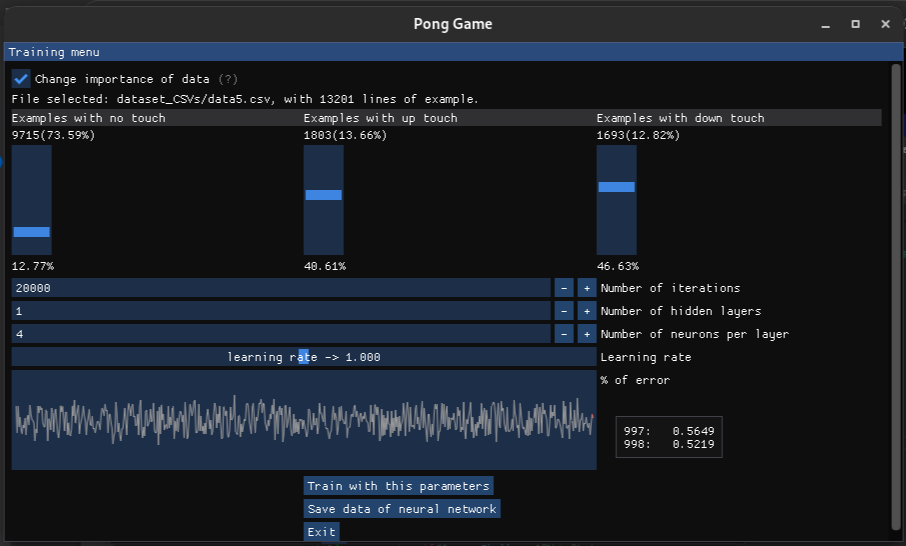
\includegraphics[width=15cm]{archivos/imagenes/menu-de-entrenamiento-alto-error.png}
		\caption{Alta importancia a pulsar.}
	\end{subfigure}

	\begin{subfigure}[h]{\textwidth}
		\centering
		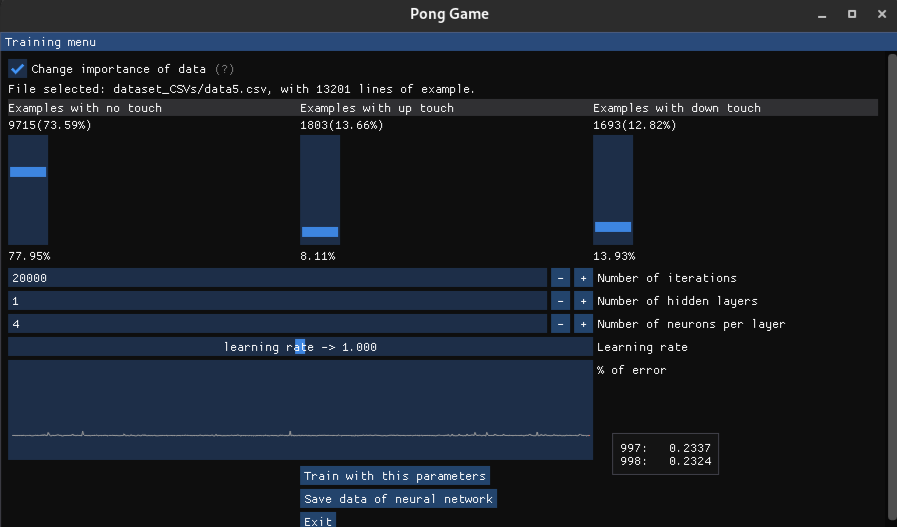
\includegraphics[width=15cm]{archivos/imagenes/menu-de-entrenamiento-bajo-error.png}
		\caption{Baja importancia a pulsar.}
	\end{subfigure}
	\caption{Comparación entre las importancias de pulsar o no pulsar.}
	\label{Comparacion alto vs bajo error}
\end{figure}

Además, la gráfica que representaba el porcentaje de error de la red neuronal de forma genérica era poco representativa, porque como vemos en la figura \ref{Comparacion alto vs bajo error}, cuando intentas que la red neuronal se comporte mejor en partida aumentando la importancia de pulsar, el error aumenta desde el 50\% hasta el 70\%. Mientras que, si lo que aumento es la importancia de no tocar (teniendo en cuenta que representa el 75\% del dataset), el error de la red permanece entre el 20\% y el 23\%. Esto puede dar una falsa imagen al usuario de que la red no está aprendiendo, por eso he separado en dos gráficas, el error que comete respecto a los ejemplos de no tocar, y el error que comete respecto a los ejemplos de sí hacerlo (figura \ref{menu dos graficas}).

\begin{figure}[H]
	\centering
	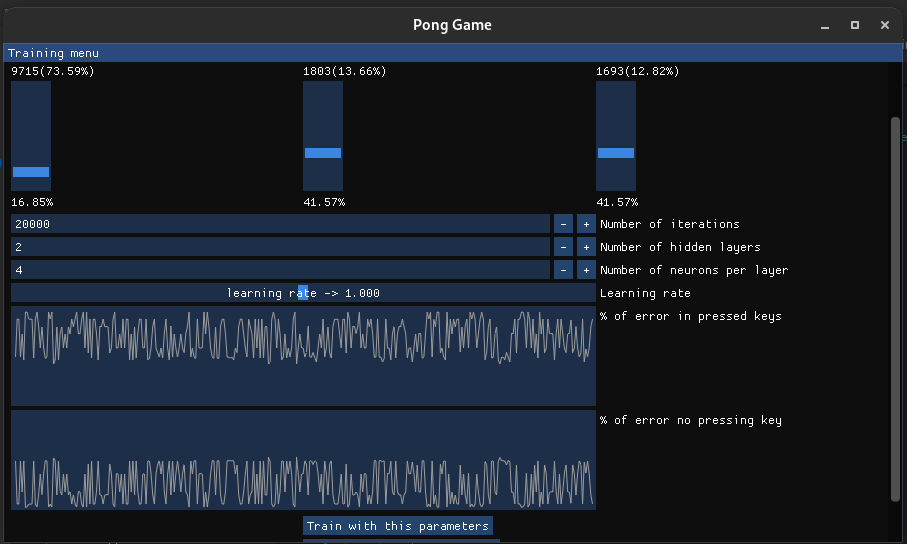
\includegraphics[width=15cm]{archivos/imagenes/menu-de-entrenamiento-dos-graficas.png}
	\caption{Menú con dos gráficas para comparar error de pulsar y no pulsar.}
	\label{menu dos graficas}
\end{figure}

\subsection{Algoritmo básico de seguimiento}
Como el usuario no tendrá ningún fichero de pesos, este necesitará un algoritmo para poder jugar contra la máquina, para poder entrenar a su bot. Por lo tanto, mi tutor y yo tuvimos la idea de darle un algoritmo por defecto a los caracteres controlados por la máquina. Escribiré un pseudocódigo para una mayor facilidad de comprensión del mismo:
\begin{lstlisting}[style=C-color, caption={Pseudocódigo de algoritmo de IA diseñada},label=macro-compile]
	Entity myself     = getMyself();
	Entity leftBall    = getLeftBall();
	Entity rightBall = getRightBall();
	
	if( (myself.x - leftBall.x)*(myself.x - leftBall.x) < 
		(myself.x - rightBall.x)*(myself.x - rightBall.x)) { //leftBall is closer
		if((myself.y - leftBall.y) > 0)
			pressDown();
		else
			pressUp();
	} else {
		if((myself.y - rightBall.y) > 0)
			pressDown();
		else
			pressUp();
	}
\end{lstlisting}
Aunque el código consta de varias lineas, es extremadamente sencillo de explicar: busca la pelota más cercana, y si está por encima en el eje y, pulsa hacia arriba. En caso contrario, hacia abajo. Desde luego no es el algoritmo más eficaz, entre otros problemas porque cuando pulsas no te mueves, sino que aceleras, pero es un sencillo algoritmo que servirá para responder algunas de las bolas antes de que el usuario haya entrenado su primera red neuronal.
 
\section{Novena iteración: los retoques finales al proyecto}
\label{novena iteracion}
El día \textbf{6 de mayo de 2021} fue la última iteración antes de decidir si entregaríamos el \gls{tfg}. Efectivamente, decidimos que sí lo haríamos, sin embargo, quedaba un duro trabajo en el mes de mayo, para acabar todas las cosas que quedaban por terminar y tener una memoria y un proyecto finalmente dignos de ser presentados ante el tribunal. Los objetivos, por lo tanto, fueron:
\begin{enumerate}
	\item Detectar y corregir el error de aprendizaje en el juego.
	\begin{itemize}
		\item Comprobar que los datos de entrada y salida se están dando bien a la red.
		\item Revisar manualmente los cálculos para algunos ejemplos.
	\end{itemize}
	\item Diferenciar entre ``gradient decent'' común y ``stochastic gradient decent''.
	\item Explicar el error en la memoria.
	\item Escribir las conclusiones en la memoria.
\end{enumerate}

El problema del aprendizaje en el juego ya había sido solventado en la octava iteración en el apartado \ref{octava iteracion}, mientras que el problema de errores en la programación ya había sido resuelto en la sexta iteración, en el apartado \ref{sexta iteracion}. Entonces, ¿qué es lo que había que corregir? ¿Por qué la red no es capaz de aprender con los datos que le aporta? Por esto es que marcamos el objetivo de ``Detectar y corregir el error de aprendizaje en el juego''.

Para mayor claridad, añadí una tercera gráfica, para ver si lo que aprendía era pulsar hacia arriba o hacia abajo. Además de un cálculo de cuántos pesos tiene en total la red, para poder determinar la dimension Vapnik-Chervonenkis, y cuántos ejemplos de cada tipo se están cogiendo en lugar de su porcentaje para mayor claridad (anteriormente era el porcentaje, pero esto aparece ahora cuando la barra es pulsada, y lo que aparece abajo es el número de muestras que tendrá de cada tipo). Figura \ref{ultimo menu de entrenamiento}.
\begin{figure}[H]
	\centering
	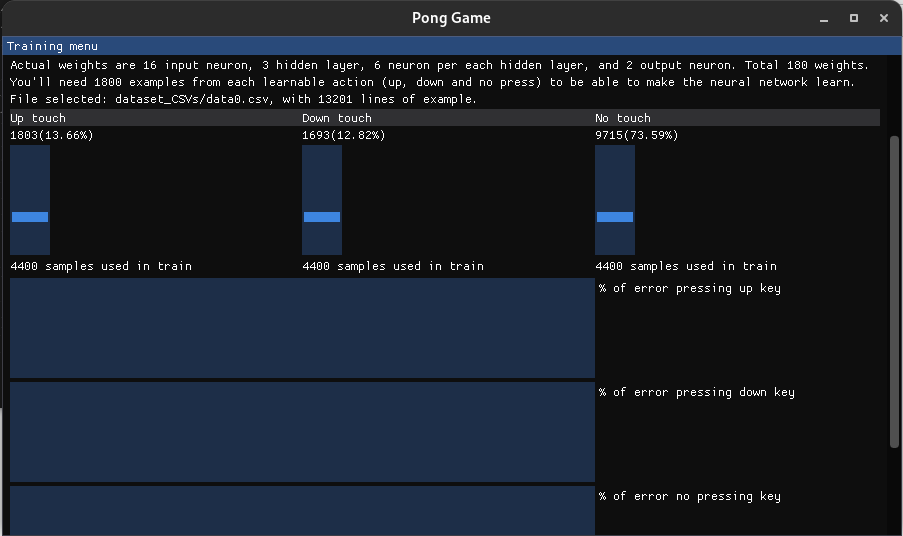
\includegraphics[width=15cm]{archivos/imagenes/menu-de-entrenamiento-definitivo.png}
	\caption{Menú de entrenamiento definitivo.}
	\label{ultimo menu de entrenamiento}
\end{figure}

Con todas las herramientas diseñadas me puse a investigar sobre los posibles errores tanto en el código (revisar las lecciones para ver si había tenido algún error de concepto), como en las muestras que se le entregan (que estuviese bien distribuido), y no encontraba ningún error. Lo más llamativo era el comportamiento de las gráficas, pues por lo general, el error de cada uno de los tipos pasaba de 100\% a 0\% de golpe entre el error denominado como "pulsar", ya sea en la tecla hacia arriba y en la tecla hacia abajo, mientras que cuando uno de estos dos pasaba a 0\% de error, el denominado como "no pulsar" pasaba a ser del 50\%. Puedes ver un ejemplo de esto en la figura \ref{error erratico}.
\begin{figure}[H]
	\centering
	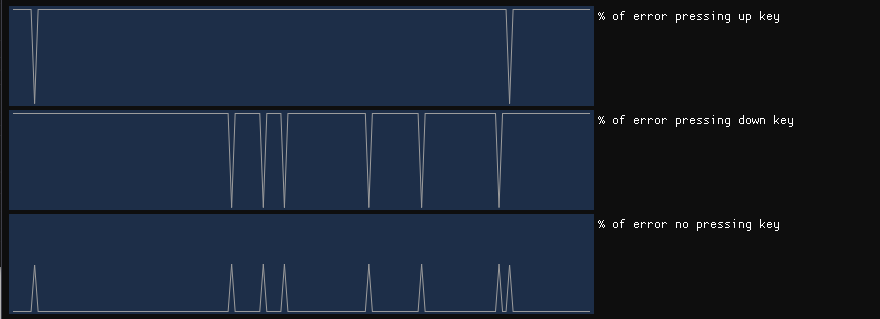
\includegraphics[width=15cm]{archivos/imagenes/error-erratico.png}
	\caption{Variación del error confusa.}
	\label{error erratico}
\end{figure}

Era, cuanto menos, curioso. Después de un tiempo probando y cambiando los distintos parámetros, conseguí que esto ya no fuera así. Usé una red más compleja que la que estaba usando comúnmente, un 20\% de ejemplos de no tocar frente al 80\% de sí hacerlo, una cantidad de iteraciones más alta, y un ratio de aprendizaje ridículamente bajo comparado con lo que estaba usando hasta ahora (acostumbrado a variar entre cero y dos, pero lo más normal era uno), 0.00185. La red comenzó a bajar el error en los tres tipos poco a poco, y no a saltos agigantados, como se aprecia en la figura \ref{error concordante}. Por lo tanto, llegué a la conclusión de que estaba aprendiendo, cosa que confirmé luego poniéndolo a prueba en el juego.
\\
Por supuesto, después de conocer el por qué del error, el rango de ratio de aprendizaje pasó de entre cero y dos, a entre cero y uno. Haciendo especial énfasis en los valores más cercanos a cero, por lo tanto ahora la barra para elegir el ratio de aprendizaje avanza de forma logaritmica (para tener más precisión con los números pequeños), en lugar de la anterior forma uniforme.
\begin{figure}[H]
	\centering
	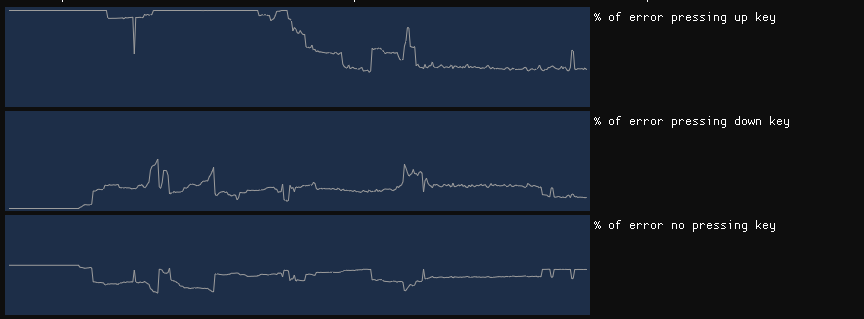
\includegraphics[width=15cm]{archivos/imagenes/error-concordante.png}
	\caption{Variación del error concordante.}
	\label{error concordante}
\end{figure}

Sin embargo, aunque ahora la red neuronal es capaz de jugar, noto que la forma en la que juega es más errática que cuando era controlada por un perceptrón, incluso más errática que el algoritmo de \gls{ia} diseñada simple que hice. Hablaré más sobre ello en el apartado de conclusiones (apartado \ref{conclusiones}).

Respecto al descenso del gradiente, estuve revisando las diferentes fuentes de información que he utilizado durante el proyecto, y he comprendido la diferencia con el modelo estocástico. Es posible que ese sea el motivo por el que la red neuronal es más errática de lo que debería. La diferencia entre el modelo común y el estocástico es que en el descenso del gradiente común, se hace la media de todos los errores de la muestra, y a partir de ahí se aplica Backpropagation, mientras que con el modelo estocástico se aplica la corrección a un subgrupo de toda la muestra. Sin embargo, aplicar esos cambios no parece que fuese a cambiar drásticamente el resultado ya que me he encargado de aleatorizar el orden de las muestras de tal forma que no pueda aprender patrones por el estado de la partida, sino solo por los datos.

Para poder depurar mejor las redes neuronales, añadí una opción en el menú principal llamada ``Edit neural network''. En ella se presentan todos los pesos de la red sin tener que manipular el fichero manualmente, cosa que podría causar errores. Puedes cambiar de una capa a la siguiente o la anterior, y variar todos los pesos de la misma. Además esta opción te dice el error que está cometiendo la red, para poder comparar si está mejorando. Puedes verla en la figura \ref{editar red neuronal}.

\begin{figure}[H]
	\centering
	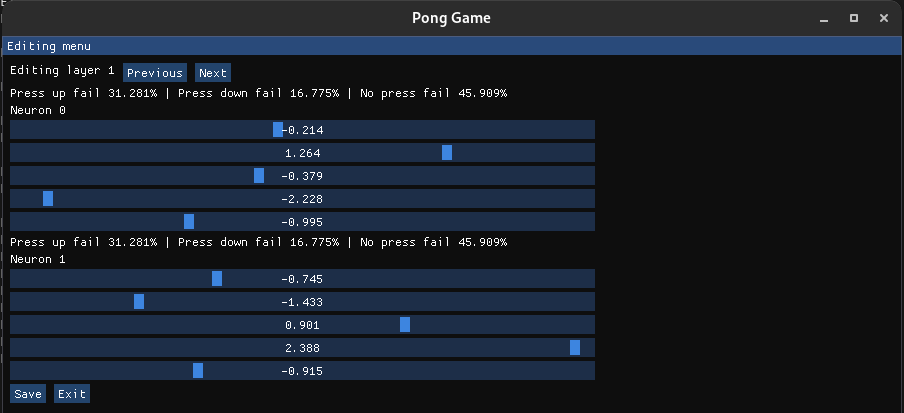
\includegraphics[width=15cm]{archivos/imagenes/menu-editar-pesos-red.png}
	\caption{Menú para editar pesos de la red neuronal.}
	\label{editar red neuronal}
\end{figure}
		% Plantilla: Se muestran listados
%%%%%%%%%%%%%%%%%%%%%%%%%%%%%%%%%%%%%%%%%%%%%%%%%%%%%%%%%%%%%%%%%%%%%%%%
% Plantilla TFG/TFM
% Escuela Politécnica Superior de la Universidad de Alicante
% Realizado por: Jose Manuel Requena Plens
% Contacto: info@jmrplens.com / Telegram:@jmrplens
%%%%%%%%%%%%%%%%%%%%%%%%%%%%%%%%%%%%%%%%%%%%%%%%%%%%%%%%%%%%%%%%%%%%%%%%
\chapter{Resultados}
\label{resultados}
En este apartado usaré comparaciones en gráficas para ver claramente las ventajas y/o inconvenientes de algunas decisiones que he tomado durante el desarrollo de este proyecto.

\section{Optimización de caché}
Como he mencionado en el desarrollo, el motor \gls{ecs} está pensado para ser ``cache-friendly''. Esto quiere decir que la memoria del programa se organiza de tal manera que optimiza la caché. Esto sucede, como ya he comentado, porque la caché lee streams de memoria, y no solo un dato. Por lo tanto, merece la pena tener los datos que vayamos a utilizar en el juego ordenados en memoria, de esta manera el juego podrá realizar más acciones por frame, debido a que la velocidad de un acceso a memoria en caché es, aproximadamente, 200 veces más rápida que un acceso a memoria RAM.

Mi primera idea para demostrar esto fue hacer un test en el cual tienes un vector de tamaño ``3x'', y tres vectores de tamaño ``x''. Supuestamente el vector del triple de tamaño conseguirá mayor velocidad al leer la memoria de forma lineal, mientras que será más lento realizar lecturas de los tres vectores, ya que el acceso a la memoria no será lineal.
\begin{lstlisting}[style=C-color, caption={Caché optimizada vs sin optimizar. Primer intento},label=cache-optimization-first]
	size_t bench_optimized(const std::vector<int>& the_one, size_t times) {
		size_t result = 0;
		
		for(std::size_t i=0; i<times; ++i) {
			for (std::size_t j = 0; j < the_one.size(); j++) {
				result += the_one[j];
			}
		}
		
		return result;
	}
	size_t bench_unoptimized(const std::vector<int>& first, const std::vector<int>& second, const std::vector<int>& third, size_t times) {
		size_t result = 0;
		
		for(std::size_t i=0; i<times; ++i) {
			for (std::size_t j = 0; j < first.size(); j++) {
				result += first[j];
				result += second[j];
				result += third[j];
			}
		}
		
		return result;
	}
\end{lstlisting}

Los resultados de este test son que el que supuestamente debería ser más lento, tarda menos tiempo en ejecutarse. Esto puede ser porque el procesador tiene varias lineas de caché, o también porque los procesadores modernos tienen instrucciones \gls{simd}, lo que hace que se puedan realizar las tres sumas de golpe y eso también explicaría una ejecución más rápida del test.
\begin{figure}[H]
	\centering
	\begin{tikzpicture}
		\begin{axis}
			[ymin=0,ymax=10000, 
			xmin=0,xmax=10000, 
			ylabel= Tiempo(ms), 
			xlabel= Nº de veces] 
			\addplot+[smooth, mark=none] coordinates 
			{(1,1) (10,12) (100,82) (1000,782) (10000,8385) (100000,83121)};
			\addplot+[smooth, mark=none] coordinates
			{(1,0) (10,7) (100,83) (1000,701) (10000,6517) (100000,72598)};
			\legend{Optim, No optim}
		\end{axis}
	\end{tikzpicture}
	\caption{Comparación de optimización vs sin optimización. Primer intento.}
\end{figure}

El siguiente ejemplo que se me ocurrió fue el típico problema de orden de lectura de datos de una matriz. He simplificado un ejemplo con el cual demostrar que el orden en el que se lee la memoria es importante. El siguiente código es una matriz, la cual se lee primero de manera "cache-friendly", y después no.
\begin{lstlisting}[style=C-color, caption={Caché optimizada vs sin optimizar. Segundo intento},label=cache-optimization-second]
size_t bench_optimized(size_t v[][width], size_t times) {
	size_t result = 0;
	
	for(size_t i=0; i<times; ++i) {
		for (size_t j = 0; j < height; ++j) 
			for (size_t k = 0; k < width; ++k)
				result += v[j][k];
	}
	
	return result;
}
size_t bench_unoptimized(size_t v[][width], size_t times) {
	size_t result = 0;
	
	for(size_t i=0; i<times; ++i) {
		for (size_t k = 0; k < width; ++k) 
			for (size_t j = 0; j < height; ++j) 
				result += v[j][k];
	}
	
	return result;
}
\end{lstlisting}

La diferencia en ambos métodos está en los dos for anidados. Una vez programados los dos métodos, procedo a hacer una comparación, y el resultado es el de la siguiente figura:
\begin{figure}[H]
	\centering
	\begin{tikzpicture}
		\begin{axis}
			[ymin=0,ymax=35000, 
			xmin=0,xmax=10000, 
			ylabel= Tiempo(ms), 
			xlabel= Nº de veces] 
			\addplot+[smooth, mark=none] coordinates 
			{(1,2) (10,32) (100,196) (1000,1949) (10000,19479)};
			\addplot+[smooth, mark=none] coordinates
			{(1,3) (10,34) (100,332) (1000,3317) (10000,33256)};
			\legend{Optim, No optim}
		\end{axis}
	\end{tikzpicture}
	\caption{Comparación de optimización vs sin optimización. Segundo intento.}
\end{figure}

El resultado es claro, en cualquier caso acceder a la memoria de forma desordenada es un 50\% más costoso en este test. Por lo que la deducción es que hay que intentar mantener la memoria ordenada para una mayor eficiencia del programa. 
\\
Un apunte final que me veo obligado a hacer es que, tanto con el compilador de clang++, como el de g++, no hay que usar el flag ``-O3''. De ser así, al ser un test tan simple, el compilador es capaz de optimizar el código máquina y los resultados de ambos test son los mismos.

\section{Aprendizaje aleatorio vs \textit{backpropagation}}
\label{aleatorio vs backpropagation resultados}
Como quiero comparar las ventajas de usar \textit{backpropagation}, lo voy a hacer contra el algoritmo más sencillo, el que tenía inicialmente, que es el algoritmo aleatorio explicado en la figura \ref{Algoritmo aleatorio}. El problema que se tratará de resolver con el algoritmo es el de la XOR, y la arquitectura que va a tener la red neuronal es dos neuronas de entrada, una capa oculta con cuatro neuronas, y una neurona de salida que dice si la entrada ha producido verdadero o falso. 
\\
Como se puede apreciar en la siguiente figura, la linea roja representa el error que tiene la red cada 10 iteraciones, y la linea azul representa cómo va mejorando el error cuando el algoritmo se guarda el mejor resultado hasta el momento. Hay que tener en cuenta que, al ser cuatro soluciones las que tiene que dar (falso y falso, falso y verdadero, verdadero y falso, verdadero y verdadero), pero hay que representar el verdadero y el false numéricamente para calcular el error de la red, un error menor al 25\% significa que ha ajustado los pesos de la red para que los cuatro casos coincidan con la solución.
\begin{figure}[H]
	\centering
	\begin{tikzpicture}
		\begin{axis}
			[ymin=0,ymax=100, 
			xmin=0,xmax=1000, 
			ylabel= \% de error, 
			xlabel= Nº de iteraciones] 
			\addplot+[smooth, mark=none] coordinates 
			{(0,99.8454) (1,97.5228) (2,95.9093) (9,42.0106) (159,34.0462) (355,22.5898) (672,18.837) (1000,18.837)};
			\addplot+[smooth, mark=none] coordinates
			{(0,99.8454) (1,97.5228) (2,95.9093) (9,42.0106) (10,74.5026)  (20,133.048) (30,50.0229) (40,92.3021) (50,100.001) (60,90.9467) (70,99.9676) (80,99.999) (90,99.994) (100,60.6559) (110,99.9855) (120,92.1943) (130,99.9257) (140,98.7933) (150,92.1119) (159,34.0462) (160,57.2305) (170,44.5407) (180,43.5673) (190,113.788) (200,100) (210,99.4142) (220,83.4381) (230,100.071) (240,58.6687) (250,82.9632) (260,99.8364) (270,62.1711) (280,59.9009) (290,99.1347) (300,90.076) (310,100) (320,99.984) (330,99.9887) (340,96.8439) (350,99.8101) (355,22.5898) (360,147.47) (370,100) (380,99.4627) (390,99.9865) (400,99.528) (410,82.7241) (420,99.9637) (430,104.989) (440,99.9984) (450,99.988) (460,90.9419) (470,98.9157) (480,59.0847) (490,99.6393) (500,99.3816) (510,83.033) (520,100) (530,89.7185) (540,97.7787) (550,98.865) (560,99.872) (570,99.9869) (580,51.2202) (590,85.9898) (600,68.4817) (610,55.4502) (620,95.9602) (630,98.2658) (640,99.2841) (650,99.8679) (660,99.999) (670,99.9999) (672,18.837) (680,52.8244) (690,98.9702) (700,99.9932) (710,97.9063) (720,55.2218) (730,99.942) (740,99.9992) (750,99.9678) (760,66.4945) (770,80.0553) (780,75.8166) (790,100.012) (800,99.9916) (810,95.3353) (820,59.7116) (830,49.9807) (840,99.9995) (850,99.9919) (860,99.9067) (870,99.9991) (880,99.9417) (890,89.8568) (900,69.0741) (910,91.0636) (920,99.9952) (930,99.9321) (940,100) (950,83.0578) (960,99.9856) (970,112.699) (980,99.9977) (990,100)};
			\legend{Mejor err, Instante err}
		\end{axis}
	\end{tikzpicture}
	\caption{Resultados del aprendizaje con un algoritmo aleatorio.}
\end{figure}

Otro dato interesante a conocer es en qué iteración el algoritmo encuentra una solución válida para resolver la XOR. El algoritmo itera 1000 veces. Después de ejecutar el algoritmo durante 10000 intentos, llego a la conclusión empírica de que el algoritmo encuentra una solución en la iteración 354.16 de media, siempre que lo encuentra. Sin embargo, hay un 19.83\% de las veces que el algoritmo aleatorio no es capaz de encontrar la solución. 
\\
Y no sólo vamos a fijarnos en el número de iteraciones que necesita el algoritmo, sino también en el tiempo, para después poder comparar con cuánto tiempo tarda contra \textit{backpropagation}. El algoritmo aleatorio tarda 12 segundos, en entrenar 10000 veces en mi máquina con optimizaciones, lo que quiere decir que de media tarda 0.0012 segundos en resolver el problema.

\begin{figure}[H]
	\centering
	\begin{tikzpicture}
		\begin{axis}
			[ymin=0,ymax=100, 
			xmin=0,xmax=1000, 
			ylabel= \% de error, 
			xlabel= Nº de iteraciones] 
			\addplot+[smooth, mark=none] coordinates 
			{(0,29.4812) (10,25.2339) (20,25.2867) (30,25.3076) (40,25.2606) (50,25.1305) (60,24.9177) (70,24.63) (80,24.28) (90,23.8848) (100,23.4652) (110,23.0428) (120,22.6349) (130,22.2486) (140,21.8801) (150,21.5146) (160,21.1258) (170,20.6836) (180,20.1719) (190,19.6021) (200,19.0071) (210,18.4247) (220,17.8803) (230,17.3789) (240,16.9021) (250,16.4006) (260,15.7806) (270,14.905) (280,13.6765) (290,12.1482) (300,10.4941) (310,08.91017) (320,07.5336) (330,06.40639) (340,05.50272) (350,04.77621) (360,04.18526) (370,03.69856) (380,03.2934) (390,02.95306) (400,02.66494) (410,02.41928) (420,02.20841) (430,02.02622) (440,01.86781) (450,01.72924) (460,01.60728) (470,01.49934) (480,01.40327) (490,01.31734) (500,01.24009) (510,01.17033) (520,01.10706) (530,01.04946) (540,0.996808) (550,0.94853) (560,0.904119) (570,0.863146) (580,0.825243) (590,0.790093) (600,0.757419) (610,0.726983) (620,0.698574) (630,0.672007) (640,0.647119) (650,0.623765) (660,0.601818) (670,0.581161) (680,0.561692) (690,0.543317) (700,0.525955) (710,0.509528) (720,0.493969) (730,0.479216) (740,0.465212) (750,0.451905) (760,0.439248) (770,0.427198) (780,0.415716) (790,0.404765) (800,0.394311) (810,0.384324) (820,0.374776) (830,0.365639) (840,0.356891) (850,0.348507) (860,0.340468) (870,0.332753) (880,0.325345) (890,0.318227) (900,0.311384) (910,0.3048) (920,0.298463) (930,0.292358) (940,0.286476) (950,0.280803) (960,0.275331) (970,0.270048) (980,0.264947) (990,0.260017)};
		\end{axis}
	\end{tikzpicture}
	\caption{Resultados del aprendizaje con el algoritmo \textit{backpropagation}.}
	\label{Resultados XOR backpropagation}
\end{figure}

En la figura \ref{Resultados XOR backpropagation} se puede ver el número de iteraciones que hay que hacer para alcanzar una solución válida es mayor, con una estructura de la red neuronal equivalente (dos neuronas de entrada, una capa oculta con cuatro neuronas, y una neurona de salida).

De los 10.000 intentos de que el algoritmo solucione el problema en 1000 iteraciones,  se consigue el 96\% de las veces, a diferencia del 80,17\% que conseguía el algoritmo aleatorio. Mientras que el tiempo que tarda el algoritmo de \textit{backpropagation} es 12 segundos, es decir, el tiempo que tarda es equivalente. Por lo tanto se demuestra que \textit{backpropagation} tiene un mayor porcentaje de acierto. De media acierta en la iteración 426, esto significa que tarda más iteraciones, sin embargo, consigue un porcentaje de acierto más alto.

La gráfica \ref{Backpropagation cambiando learning rate} muestra, ya que \textit{backpropagation} tiene un parámetro para ajustar el ratio de aprendizaje, una comparación entre diferentes posibles valores del mismo. 
\begin{figure}[H]
	\centering
	\begin{tikzpicture}
		\begin{axis}
			[ymin=0,ymax=100, 
			xmin=0,xmax=1000, 
			ylabel= \% de error, 
			xlabel= Nº de iteraciones] 
			\addplot+[smooth, mark=none, color=red] coordinates 
			{(0,29.512) (10,28.1277) (20,27.1086) (30,26.4112) (40,25.9586) (50,25.6752) (60,25.5017) (70,25.3968) (80,25.3338) (90,25.296) (100,25.2732) (110,25.2593) (120,25.2506) (130,25.245) (140,25.2412) (150,25.2385) (160,25.2364) (170,25.2346) (180,25.233) (190,25.2316) (200,25.2302) (210,25.2288) (220,25.2274) (230,25.226) (240,25.2246) (250,25.2232) (260,25.2218) (270,25.2203) (280,25.2188) (290,25.2173) (300,25.2158) (310,25.2143) (320,25.2127) (330,25.2111) (340,25.2095) (350,25.2079) (360,25.2062) (370,25.2046) (380,25.2029) (390,25.2011) (400,25.1994) (410,25.1976) (420,25.1959) (430,25.194) (440,25.1922) (450,25.1904) (460,25.1885) (470,25.1866) (480,25.1847) (490,25.1828) (500,25.1808) (510,25.1789) (520,25.1769) (530,25.1749) (540,25.1728) (550,25.1708) (560,25.1687) (570,25.1666) (580,25.1645) (590,25.1624) (600,25.1602) (610,25.1581) (620,25.1559) (630,25.1537) (640,25.1514) (650,25.1492) (660,25.1469) (670,25.1446) (680,25.1423) (690,25.14) (700,25.1377) (710,25.1353) (720,25.133) (730,25.1306) (740,25.1282) (750,25.1257) (760,25.1233) (770,25.1209) (780,25.1184) (790,25.1159) (800,25.1134) (810,25.1109) (820,25.1083) (830,25.1058) (840,25.1032) (850,25.1006) (860,25.098) (870,25.0954) (880,25.0927) (890,25.0901) (900,25.0874) (910,25.0848) (920,25.0821) (930,25.0794) (940,25.0766) (950,25.0739) (960,25.0711) (970,25.0684) (980,25.0656) (1000,25.0628)};
			\addplot+[smooth, mark=none, color=green] coordinates 
			{(0,29.3) (10,25.0566) (20,25.0105) (30,24.9931) (40,24.9757) (50,24.9583) (60,24.9408) (70,24.9229) (80,24.9045) (90,24.8853) (100,24.8651) (110,24.8438) (120,24.8211) (130,24.7969) (140,24.771) (150,24.7431) (160,24.7133) (170,24.6812) (180,24.6469) (190,24.6101) (200,24.5708) (210,24.5288) (220,24.4839) (230,24.4362) (240,24.3855) (250,24.3317) (260,24.2747) (270,24.2146) (280,24.1512) (290,24.0846) (300,24.0148) (310,23.942) (320,23.8661) (330,23.7874) (340,23.706) (350,23.6222) (360,23.5363) (370,23.4484) (380,23.3591) (390,23.2686) (400,23.1774) (410,23.0858) (420,22.9944) (430,22.9037) (440,22.8142) (450,22.7264) (460,22.6408) (470,22.5582) (480,22.479) (490,22.4039) (500,22.3336) (510,22.2686) (520,22.2098) (530,22.1577) (540,22.113) (550,22.0762) (560,22.0479) (570,22.0285) (580,22.0179) (590,22.0159) (600,22.0221) (610,22.0353) (620,22.0543) (630,22.0773) (640,22.1026) (650,22.1284) (660,22.1531) (670,22.1756) (680,22.195) (690,22.2107) (700,22.2226) (710,22.2307) (720,22.2353) (730,22.2368) (740,22.2355) (750,22.2319) (760,22.2266) (770,22.22) (780,22.2129) (790,22.2058) (800,22.1999) (810,22.1961) (820,22.1962) (830,22.202) (840,22.2161) (850,22.2416) (860,22.282) (870,22.3408) (880,22.4211) (890,22.5251) (900,22.6531) (910,22.8037) (920,22.9734) (930,23.1577) (940,23.3517) (950,23.5513) (960,23.7536) (970,23.9572) (980,24.1618) (1000,24.3679)};
			\addplot+[smooth, mark=none, color=blue] coordinates 
			{(0,28.248) (10,25.3732) (20,25.2915) (30,25.2241) (40,25.1636) (50,25.106) (60,25.0469) (70,24.9828) (80,24.9108) (90,24.8282) (100,24.7322) (110,24.6193) (120,24.4855) (130,24.3261) (140,24.1353) (150,23.9066) (160,23.6327) (170,23.3063) (180,22.9209) (190,22.472) (200,21.9589) (210,21.3852) (220,20.76) (230,20.0981) (240,19.4208) (250,18.7547) (260,18.1179) (270,17.4745) (280,16.668) (290,15.4365) (300,13.6576) (310,11.5672) (320,9.54095) (330,7.80622) (340,6.41307) (350,5.32242) (360,4.47286) (370,3.80792) (380,3.28268) (390,2.86313) (400,2.52397) (410,2.24648) (420,2.01678) (430,1.82452) (440,1.66192) (450,1.52308) (460,1.40347) (470,1.29961) (480,1.20875) (490,1.12873) (500,1.05781) (510,0.99461) (520,0.937991) (530,0.887026) (540,0.840947) (550,0.799118) (560,0.761003) (570,0.726151) (580,0.694179) (590,0.664761) (600,0.637618) (610,0.612507) (620,0.58922) (630,0.567575) (640,0.547413) (650,0.528595) (660,0.511) (670,0.494518) (680,0.479055) (690,0.464524) (700,0.450851) (710,0.437968) (720,0.425814) (730,0.414336) (740,0.403484) (750,0.393213) (760,0.383486) (770,0.374266) (780,0.36552) (790,0.357219) (800,0.349336) (810,0.341849) (820,0.334734) (830,0.327972) (840,0.321545) (850,0.315437) (860,0.309633) (870,0.304121) (880,0.298888) (890,0.293925) (900,0.28922) (910,0.284768) (920,0.280559) (930,0.276588) (940,0.27285) (950,0.269339) (960,0.266052) (970,0.262985) (980,0.260136) (1000,0.257503)};
			\addplot+[smooth, mark=none, color=black] coordinates 
			{(0,25.6122) (10,25.2806) (20,25.5486) (30,26.1927) (40,26.2346) (50,23.2293) (60,21.0663) (70,19.7438) (80,26.8959) (90,19.8321) (100,15.9827) (110,8.20897) (120,3.12829) (130,1.71361) (140,1.12593) (150,0.824623) (160,0.644778) (170,0.526445) (180,0.443183) (190,0.381668) (200,0.334504) (210,0.297276) (220,0.267194) (230,0.242415) (240,0.221673) (250,0.204072) (260,0.18896) (270,0.175852) (280,0.16438) (290,0.154262) (300,0.145274) (310,0.137241) (320,0.130019) (330,0.123495) (340,0.117572) (350,0.112173) (360,0.107232) (370,0.102695) (380,0.0985132) (390,0.0946486) (400,0.0910663) (410,0.0877371) (420,0.0846355) (430,0.0817391) (440,0.0790285) (450,0.0764867) (460,0.0740986) (470,0.0718509) (480,0.0697316) (490,0.0677303) (500,0.0658374) (510,0.0640446) (520,0.0623441) (530,0.0607292) (540,0.0591936) (550,0.0577316) (560,0.0563383) (570,0.0550088) (580,0.053739) (590,0.0525251) (600,0.0513633) (610,0.0502506) (620,0.0491838) (630,0.0481603) (640,0.0471775) (650,0.0462329) (660,0.0453246) (670,0.0444504) (680,0.0436085) (690,0.0427971) (700,0.0420147) (710,0.0412597) (720,0.0405307) (730,0.0398265) (740,0.0391458) (750,0.0384874) (760,0.0378503) (770,0.0372335) (780,0.036636) (790,0.036057) (800,0.0354956) (810,0.0349511) (820,0.0344226) (830,0.0339096) (840,0.0334113) (850,0.0329271) (860,0.0324565) (870,0.0319988) (880,0.0315537) (890,0.0311205) (900,0.0306988) (910,0.0302881) (920,0.0298881) (930,0.0294983) (940,0.0291183) (950,0.0287478) (960,0.0283865) (970,0.0280339) (980,0.0276899) (1000,0.027354)};
			\addplot+[smooth, mark=none, color=yellow] coordinates 
			{(0,42.4898) (10,26.8803) (20,22.8098) (30,20.214) (40,19.1996) (50,18.6843) (60,18.3622) (70,18.0976) (80,17.5636) (90,16.6035) (100,16.0297) (110,14.9599) (120,14.8262) (130,19.9627) (140,19.5791) (150,21.4538) (160,21.875) (170,22.0504) (180,23.7649) (190,24.4441) (200,19.458) (210,0.317342) (220,0.254418) (230,0.212609) (240,0.18255) (250,0.159892) (260,0.142216) (270,0.128057) (280,0.116475) (290,0.106839) (300,0.0987078) (310,0.0917677) (320,0.0857866) (330,0.0805911) (340,0.0760492) (350,0.0720591) (360,0.0685418) (370,0.0654361) (380,0.0626946) (390,0.0602823) (400,0.0581747) (410,0.0563583) (420,0.0548319) (430,0.05361) (440,0.0527314) (450,0.0522758) (460,0.0524051) (470,0.0534717) (480,0.0563899) (490,0.0645567) (500,0.117378) (510,19.4729) (520,19.3731) (530,19.3201) (540,19.2874) (550,19.2651) (560,19.2491) (570,19.2369) (580,19.2275) (590,19.2199) (600,19.2136) (610,19.2085) (620,19.2041) (630,19.2003) (640,19.1971) (650,19.1943) (660,19.1918) (670,19.1896) (680,19.1876) (690,19.1858) (700,19.1842) (710,19.1828) (720,19.1815) (730,19.1803) (740,19.1792) (750,19.1782) (760,19.1773) (770,19.1764) (780,19.1757) (790,19.1749) (800,19.1742) (810,19.1736) (820,19.173) (830,19.1725) (840,19.172) (850,19.1715) (860,19.1711) (870,19.1706) (880,19.1703) (890,19.1699) (900,19.1695) (910,19.1692) (920,19.1689) (930,19.1686) (940,19.1684) (950,19.1681) (960,19.1679) (970,19.1677) (980,19.1675) (1000,19.1673)};
			\legend{0.05, 0.5, 1, 5, 15}
		\end{axis}
	\end{tikzpicture}
	\caption{Resultados del aprendizaje con el algoritmo \textit{backpropagation}, según el learning rate.}
	\label{Backpropagation cambiando learning rate}
\end{figure}

Se aprecia que ratios de aprendizaje extremadamente bajos y extremadamente altos hacen que la red no aprenda bien, por diferentes motivos. No se puede decir un ratio que sea común para todos los problemas, por eso en el juego dejo experimentar al usuario con distintos ratios para que encuentre el mejor. 

\section{\textit{Backpropagation} en el juego}
Como ya he comentado, he tenido problemas en el aprendizaje dentro del juego. La red neuronal no aprendía tan bien como en el problema de la XOR, y finalmente descubrí que era a causa, entre otras cosas, del \textit{learning rate} mayormente. Y como se puede ver en la figura \ref{error erratico}, valores cercanos a uno provocan que la red no sea capaz de aprender. Pero depurando más profundamente, detecto lo que puede ser la explicación al error.

Con una arquitectura de la red de 16 entradas, una capa intermedia de 4 neuronas y 2 salidas, para un valor de \textit{learning rate} alto (cercano a uno) sucede lo que se puede ver en la figura \ref{alto learning rate arquitectura simple}. Los pesos de la primera capa (la que conecta las 16 neuronas con las 4) mantienen los valores obtenidos aleatoriamente, no varían en todo el entrenamiento, mientras que los de la segunda capa (la que conecta las 4 neuronas con las 2 de salida) sí que lo hacen. Sin embargo, si uso un ratio de aprendizaje menor a 0.001, ambas capas de pesos cambian, pero sigo sin conseguir un resultado satisfactorio, una arquitectura tan simple no es capaz de aprender a jugar, pero sí que varían los parámetros de la primera capa.

\begin{figure}[H]
	\centering
	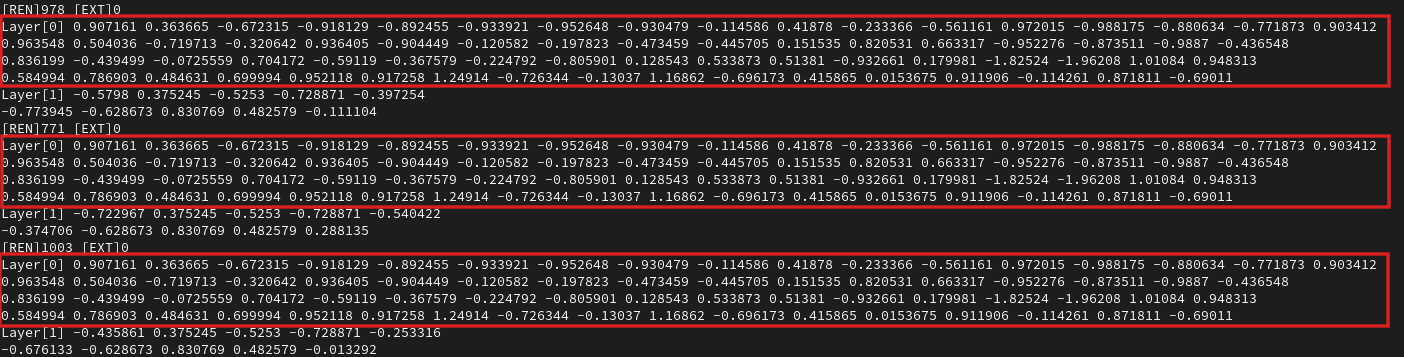
\includegraphics[width=15cm]{archivos/imagenes/alto-learning-rate-arquitectura-simple.png}
	\caption{Varianza de peso en arquitectura simple con un learning rate alto.}
	\label{alto learning rate arquitectura simple}
\end{figure}

Ahora pruebo con una arquitectura más compleja, 16 neuronas de entrada, 4 capas ocultas de 6 neuronas cada una, y 2 neuronas de salida. Además un total de 10000 iteraciones, y la distribución de la muestra es aproximadamente 40\% muestras de tocar arriba, 40\% muestras de tocar abajo, y 20\% muestras de no tocar. Para valores cercanos a uno sigue sucediendo lo visto en la figura \ref{error erratico}, y además, sucede lo mismo que en la figura \ref{alto learning rate arquitectura simple}, que la primera capa no varía, mientras que el resto sí que lo hace. Sin embargo, para un valor del ratio de aprendizaje menor a 0.001, la red si que aprende y sucede lo que puedes ver en la figura \ref{error concordante}, obtenemos errores bajos corregidos a lo largo de las 10000 iteraciones en los tres gráficos, y cuando ponemos la red resultante a jugar, lo hace de manera satisfactoria. 

\begin{figure}[H]
	\centering
	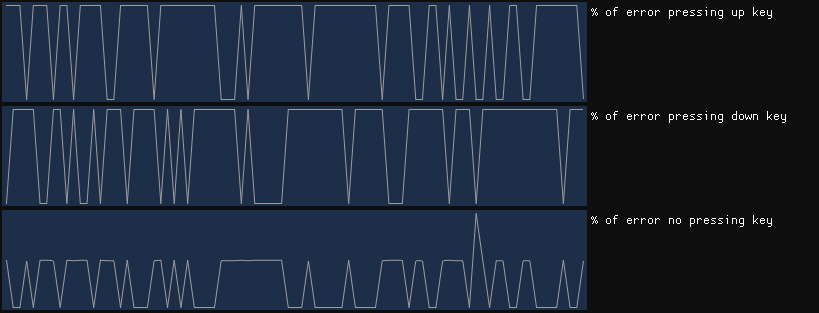
\includegraphics[width=15cm]{archivos/imagenes/arquitectura-compleja-learning-rate-alto.png}
	\caption{Porcentaje de acierto con arquitectura compleja y learning rate alto.}
	\label{alto learning rate arquitectura compleja}
\end{figure}

Por último, pongo a entrenar a la red más compleja que permite el juego. Será una arquitectura de 16 neuronas de entrada, 10 capas ocultas con 10 neuronas cada una, y con 2 neuronas de salida.  Diez mil iteraciones como antes, y un ratio de aprendizaje del 0.743. Lo que pasa en este caso es que, sorprendentemente, cambian todos los pesos de todas las capas (incluida la primera capa), pero las últimas capas cambian mucho más rápido que las primeras (como ha sucedido también en los anteriores ejemplos). Los resultados de las gráficas son muy parecidos a los ya comentados antes con learning rate alto, pero he tomado otra captura que puedes ver en la figura \ref{alto learning rate arquitectura compleja} para dejarlo demostrado.

Lo siguiente que hago es poner a entrenar la misma arquitectura, pero con un learning rate de 0.0074 durante diez mil iteraciones, y una distribución de los datos 40-40-20 como ya he comentado antes. Todos los pesos  de todas las capas están variando, pero con una velocidad de cambio menor. El resultado final de esta red tan compleja es el que se puede ver en la figura \ref{bajo learning rate arquitectura compleja}, \textit{backpropagation} no es capaz de corregir el error con este número de iteraciones, y lo más normal será que se quede con un 0\% de error ``no pulsar'' y 100\% ``pulsar'', porque al generar la red de manera aleatoria, es lo más probable. Los resultados son los mismos con un valor de learning rate intermedio como 0.359.
\begin{figure}[H]
	\centering
	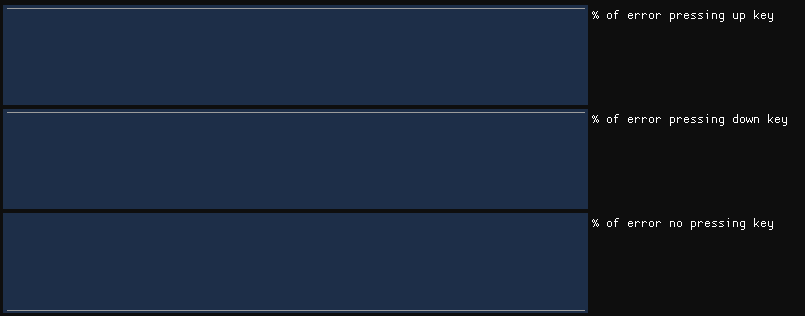
\includegraphics[width=15cm]{archivos/imagenes/arquitectura-compleja-learning-rate-bajo.png}
	\caption{Porcentaje de acierto con arquitectura compleja y learning rate bajo.}
	\label{bajo learning rate arquitectura compleja}
\end{figure}

En última instancia he querido comprobar si la red se comportaba mejor con un número menor de entradas. En principio esto no debería afectar mucho según la teoría de la dimensión Vapnik-Chervonenkis porque el número de términos independientes es prácticamente el mismo, sin embargo, los resultados no dicen lo mismo. Los datos que se le pasan a la red original del juego son, la posición x e y, velocidades x e y, y la aceleración tanto del agente, como de las pelotas, como del minion mas cercano. La aceleración sólo al minion y el agente, que son los que la aplican al pulsar para moverse.
\\
El primer intento fue quitar la aceleración como entrada, comprobé que durante el entrenamiento se cometía menos fallos, pero a la hora de jugar era similar. El segundo intento fue quitar también los valores del minion, mismo resultado que al principio. Y por último decidí dejar sólo como entrada la posición x e y del agente y las dos pelotas. En este último intento sí que noté algo de mejoría en la forma de jugar, el agente había aprendido a jugar casi tan acertado como cuando solo había dos perceptrones. Y aunque el número de términos independientes sea prácticamente el mismo, sí que hay una explicación para este suceso: el agente aprende mejor porque las posiciones x e y son los datos más relevantes de la muestra, aunque se puede extraer información interesante del resto de datos, el agente será capaz de extraer más fácilmente el ruido de la muestra si sólo pongo los datos más relevantes como entradas a la red.		% Plantilla: Se muestran gráficas
%%%%%%%%%%%%%%%%%%%%%%%%%%%%%%%%%%%%%%%%%%%%%%%%%%%%%%%%%%%%%%%%%%%%%%%%
% Plantilla TFG/TFM
% Escuela Politécnica Superior de la Universidad de Alicante
% Realizado por: Jose Manuel Requena Plens
% Contacto: info@jmrplens.com / Telegram:@jmrplens
%%%%%%%%%%%%%%%%%%%%%%%%%%%%%%%%%%%%%%%%%%%%%%%%%%%%%%%%%%%%%%%%%%%%%%%%

\chapter{Conclusiones (Con ejemplos de matemáticas)}
\label{conclusiones}

\todo{¿Hace falta poner alguna conclusión?¿O basta con el apartado de resultados?¿Hay alguna diferencia entre ellos?}	% Plantilla: Se muestran matemáticas

%%%%
% CONTENIDO. BIBLIOGRAFÍA.
%%%%
\nocite{*} %incluye TODOS los documentos de la base de datos bibliográfica sean o no citados en el texto
\bibliography{bibliografia/bibliografia} % Archivo que contiene la bibliografía
\bibliographystyle{apacite}

%%%%
% CONTENIDO. LISTA DE ACRÓNIMOS. Comenta las líneas si no lo deseas incluir.
%%%%
% Incluuye el listado de acrónimos utilizados en el trabajo. 
\printglossary[style=modsuper,type=\acronymtype,title={Lista de Acrónimos}]
% Añade el resto de acrónimos si así se desea. Si no elimina el comando siguiente
\glsaddall

%%%%
% CONTENIDO. Anexos - Añade o elimina según tus necesidades
%%%%
\appendix % Inicio de los apéndices
%%%%%%%%%%%%%%%%%%%%%%%%%%%%%%%%%%%%%%%%%%%%%%%%%%%%%%%%%%%%%%%%%%%%%%%%
% Plantilla TFG/TFM
% Escuela Politécnica Superior de la Universidad de Alicante
% Realizado por: Jose Manuel Requena Plens
% Contacto: info@jmrplens.com / Telegram:@jmrplens
%%%%%%%%%%%%%%%%%%%%%%%%%%%%%%%%%%%%%%%%%%%%%%%%%%%%%%%%%%%%%%%%%%%%%%%%

\chapter{Anexo}
\section{Vicisitudes durante el desarrollo}
El primer problema que me gustaría comentar en el anexo fue la sobrestimación de mis capacidades. Por lo que me ha comentado mi tutor, es algo que suele pasar, sobretodo cuando eres una persona sin experiencia en el sector. Desde el principio del proyecto apunté a hacer cosas que eran extremadamente difíciles, pero por suerte mi tutor supo cómo orientarme en el camino y pararme los pies en ciertos momentos, ya que de no haber sido así, es probable que no hubiese acabado el proyecto. 
\\
Otra parte en la que sobreestimé mis capacidades fue a la hora de desarrollar el motor de videojuegos. Ciertamente comencé a ver las clases de \cite{CursoMotorC++} en verano, pero cuando comenzó el curso fue cuando comencé a desarrollarlo. Pensaba que en un mes de trabajo habría terminado, sin embargo, no fue hasta mediados de noviembre que terminé por completo el desarrollo del mismo. Por supuesto, sin contar las posteriores correcciones.
\\
Además, también sobreestimé mis conocimientos sobre estadística, probabilidad y programación. Es cierto que es algo que siempre me han gustado, y a raíz de eso y tener tanto relación con la \gls{ia}, fue por lo que elegí el tema del \gls{tfg}, pero entender y desarrollar el algoritmo de \textit{backpropagation} fue algo que me llevó mucho más tiempo del que habría imaginado.

Otro de los problemas fue la pérdida del proyecto. Como ya he mencionado en el apartado de herramientas de trabajo, yo he desarrollado este proyecto con Linux, pero por motivos relacionados con la carrera, es necesario que también tenga instalado Windows en el ordenador. Después de una actualización, este último dejó de funcionar, y cuando opté por solucionar el error, se cargó la partición de Linux. Por suerte, todo el trabajo del \gls{tfg} estaba bajo el control de Git, y en la nube de GitHub, por lo que los daños en ese sentido eran mínimos. Pero tuve que invertir una cantidad de tiempo considerable en recuperar el resto de cosas de mi ordenador que no tenían una copia de seguridad alguna. Desde luego que ahora tengo más cuidado con hacer copias de seguridad de las cosas importantes.
\\
No voy a contar cómo fue la recuperación del sistema operativo ya que no procede en esta memoria, pero esto juntado con los trabajos de las asignaturas de la universidad, me hizo perder más de una semana.

Por último quiero comentar que este largo desarrollo ha sido posible porque este es mi quinto año de carrera, sólo tenía dos asignaturas que cursar en todo el año, y por eso me he permitido la licencia de dedicarle tanto tiempo al proyecto. Por otro lado, si ya hubiese tenido conocimientos previos más avanzados sobre \gls{ia}, y sobre motores de videojuegos, el desarrollo podría haberse acortado meses, sin embargo, es algo que he hecho con ganas y me ha servido para tener una experiencia que tendrá mucha utilidad en mi futuro.

\section{Cómo probar el juego}
Puede darse el caso de que quieras probar el juego, por lo que te daré las instrucciones para compilarlo, y además, los controles del juego.
Compilar es tan sencillo como entrar en la carpeta donde se ubique el Makefile y ejecutar desde una terminal \texttt{make libs \&\& make}, se generará un ejecutable llamado game y tendrás que ejecutar desde ese mismo directorio \texttt{./game}. Sin embargo, puede que tengas algún problema en la compilación, siempre y cuando no tengas instalado X11, GLFW, OpenGL y GLEW. Para instalar estas librerías en Linux, dependerá de tu distribución, pero lo que tienes que hacer es buscar con tu gestor de paquetes cómo se llaman en tu distribución estas librerías y descargarlas.

Para jugar al juego, una vez compilado, lo que harás será seleccionar la opción ``Play'', esta sirve para jugar una \gls{ia} contra otra. Mientras que la opción ``Arena'', sirve para recoger datos en un archivo dataset, con el cual podrás entrar en la siguiente opción llamada ``Train''. Esta última te llevará a un nuevo menú en el que podrás ajustar diferentes parámetros para el entrenamiento mediante \textit{backpropagation}. Todo esto se ve en la figura \ref{Menu inicial definitivo}.
\begin{figure}[H]
	\centering
	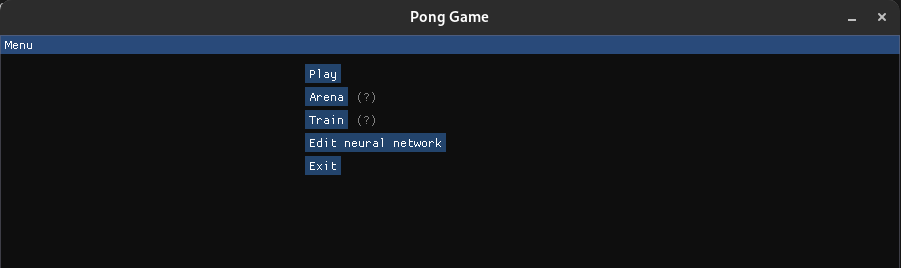
\includegraphics[width=15cm]{archivos/imagenes/menu-inicia-definitivo.png}
	\caption{Menú inicial definitivo.}
	\label{Menu inicial definitivo}
\end{figure}

En el menú de entrenamiento aparecen los ajustes recomendados, pero puedes variarlos para probar cómo cambia el error de la red en tiempo real, tanto el \textit{learning rate} como la cantidad de muestras de cada tipo que se le entregan al agente durante el entrenamiento.

Por último, las teclas para manejar al jugador de la izquierda son \textbf{w} y \textbf{s}, y para el jugador de la derecha son \textbf{o} y \textbf{l}.

\end{document}
